\documentclass[a4paper,11pt]{report}

%TexLive pakker
\usepackage[utf8]{inputenc}
\usepackage[T1]{fontenc}
\usepackage{lmodern}
\usepackage[norsk]{babel}
\usepackage{parskip}
\usepackage{graphicx}
\usepackage{caption}
\usepackage{subcaption}
\usepackage{titlepic}
\usepackage{a4wide}
\usepackage{lettrine}
\usepackage[htt]{hyphenat}
\usepackage{enumitem}
\usepackage{color}
\usepackage{hyperref}
\usepackage{listings}
\usepackage[section]{placeins}
% xcolor og fix-cm brukes til fremsiden
\usepackage{xcolor} 
\usepackage{fix-cm}
 
\lstdefinestyle{java1}{
  language=Java,
  basicstyle={\ttfamily\footnotesize},
  numberstyle={\ttfamily\footnotesize},
  keywordstyle={\ttfamily\footnotesize\color[rgb]{0,0,1}},
  commentstyle={\ttfamily\footnotesize\color[rgb]{0.133,0.545,0.133}},
  stringstyle={\ttfamily\footnotesize\color[rgb]{0.627,0.126,0.941}},
  breaklines=true,
  columns=fixed,
  extendedchars=true,
  numbers=left,
  numbersep=3pt,
  showspaces=false,
  showstringspaces=false,
  stepnumber=1,
  tabsize=2
}
\lstset{style=java1,
literate=%
{æ}{{\ae}}1
{å}{{\aa}}1
{ø}{{\o}}1
{Æ}{{\AE}}1
{Å}{{\AA}}1
{Ø}{{\O}}1
}
\renewcommand\lstlistingname{Eksempel}
\renewcommand\lstlistlistingname{Eksempler}

\usepackage[Bjornstrup]{fncychap}

\usepackage{fancyhdr}
\setlength{\headheight}{15.2pt}
\pagestyle{fancy}
\fancypagestyle{plain}{ %
  \fancyhf{} % remove everything
  \renewcommand{\headrulewidth}{0pt} % remove lines as well
  \renewcommand{\footrulewidth}{0pt}
}

%Her kommer opsett av info for pdf filen 
% \pdfinfo{%
%  /Title    (Rapport prosjektoppgave i programutvikling)
%  /Author   ()
%  /Creator  ()
%  /Producer ()
%  /Subject  ()
%  /Keywords ()
% }



\begin{document}
\setlength{\oddsidemargin}{0mm} % Adjust margins to center the colored title box
\setlength{\evensidemargin}{0mm} % Margins on even pages - only necessary if adding more content to this template

\newcommand{\HRule}[1]{\hfill \rule{0.2\linewidth}{#1}} % Horizontal rule at the bottom of the page, adjust width here

\definecolor{grey}{rgb}{0.9,0.9,0.9} % Color of the box surrounding the title - these values can be changed to give the box a different color	


\thispagestyle{empty} % Remove page numbering on this page

%----------------------------------------------------------------------------------------
%	TITLE SECTION
%----------------------------------------------------------------------------------------

\colorbox{grey}{
	\parbox[t]{1.0\linewidth}{
		\centering \fontsize{50pt}{80pt}\selectfont % The first argument for fontsize is the font size of the text and the second is the line spacing - you may need to play with these for your particular title
		\vspace*{0.7cm} % Space between the start of the title and the top of the grey box
		
% 		\hfill Logo \\
		\hfill 
\includegraphics[width=80mm]{./img/fremside/logo.png} \\
		%\hfill EasyDev \\
		\hfill 
		\fontsize{30pt}{50pt}\selectfont 
		{\fontfamily{phv}\selectfont 
		TuxMin%
		}
		\par
		
		\vspace*{0.7cm} % Space between the end of the title and the bottom of the grey box
	}
}

%----------------------------------------------------------------------------------------

\vfill % Space between the title box and author information

%----------------------------------------------------------------------------------------
%	AUTHOR NAME AND INFORMATION SECTION
%----------------------------------------------------------------------------------------

{\centering \large 
\hfill Espen Zaal s198599 \\
\hfill Petter Knagenhjelm Lysne s198579 \\
\hfill Lukas David Larsed s198569 \\


\HRule{1pt}} % Horizontal line, thickness changed here

%----------------------------------------------------------------------------------------

\clearpage % Whitespace to the end of the page

% Her kommer sammendrag som skal være det som kommer først etter fremsiden.  
\begin{abstract}
\lettrine[lines=3]{Å} summere to måneders hardt arbeid ned på en side eller to er vanskelig. Det begynte ganske så greit. Det var en god del diskusjoner den første tiden på hvordan programmet skulle se ut. Spesielt dette med at vi må simulere en virkelighet der man ser for seg boligsøker som sitter hjemme og søker etter boliger, og megler har kontrollen på resten. Det var litt vrient å velge hvordan man skulle tolke oppgaven sånn sett. Den ga mye frihet, og resultatet vi har kommet frem til nå mot slutten er helt annerledes enn det vi opprinnelig skisserte i de første tegningene.

Vi endte opp med en løsning der boligsøker utfører søkene sine i sitt panel, og om en finner en interessant annonse så kan en søke på den. Boligsøker må bekrefte utleier sine krav for boligen før søknaden havner i søknadslisten hos megler. Megler på sin side har myndighet fra utleier til å både opprette boligobjektene og annonsene, samt godkjenne den søknaden han mener er det beste alternativet. Megler skriver så kontrakt med rett boligsøker, på vegne av utleier.

På et tidspunkt før vi begynte selve utviklingen satt vi av en god uke der vi hver for oss skulle lære så mye om \texttt{Swing} som mulig. På de tidspunktet hadde vi ikke nok grunnkunnskap om hva som er mulig rent teknisk og hva vi realistisk kunne få til innenfor tidsrammen.

MVC-arkitektur ble raskt besluttet at vi skulle ha. Skrekkhistorier om java-filer på flere tusen rader, samt at ingen av dem ville kunne gjenbrukes var ikke fristende. Dette var en stor inspirasjonskilde for videre læring og utvikling. Vi ble raskt vant til å finne flere kilder til informasjon enn bare pensum, da våre utfordringer ofte lå godt utenfor pensum.

MVC er egentlig lagdelt arkitektur. Datalaget, brukergrensesnittet og logikken, hver for seg i forskjellige lag, der logikklaget styrer all funksjonalitet. Bare ved å ha de samme to kontrollerne \texttt{ControllerTabell.java} og \texttt{ControllerOutput.java} til å virke både i meglervindu og annonsevindu har vi spart ca 2000 kodelinjer, samt betydelig med tid i forhold til å slippe å oppdatere samme funksjonalitet flere steder.
Når vi nå nærmer oss slutten på prosjektet, har vi dekket hele oppgavens krav om implementasjon av teknologi, men samtidig lagt til rette for å kunne utvide programmet videre.

Ser man på selve gruppearbeidet og prosessen vår som gruppe, så er det en del lærdom å ta med seg derfra. Det krever mye erfaring å få en gruppe til å være mest mulig produktiv. Å fordele oppgaver som både gir mening og som tar prosjektet fremover er vanskelig, og da alle i gruppen lærte mye av de tekniske underveis, ble det ikke så effektivt som ønskelig.

Om en skal summere prosjektet som helhet, er alle i gruppen fornøyde med resultatet. Allerede nå ser vi forbedringer man gjerne skulle gjort om man hadde hatt tid, eller kunne begynt på nytt, men kompleksiteten av de vi har implementert og mengden funksjonalitet som er implementert er vi godt fornøyd med.




\end{abstract}
\tableofcontents
\lstlistoflistings
\listoffigures
\listoftables

%Her kommer alle linker til våre kapitel

\chapter{Introduksjon}

\section{Om rapporten}
Denne rapporten består av flere kapitler som kan leses hver for seg og som har hvert sine formål.


\begin{description}

\item[Introduksjonen] vil gå gjennom litt av forutsetningene for oppgaven, målene vi har satt oss, tolkningen av oppgaven og valgene vi har tatt på bakgrunn av det. 

\item[Prosessdokumentasjonen] vil beskrive aspektet ved arbeidet vårt. Hvordan vi kom sammen som en gruppe, bestemte oss for fremgangsmåte og utfordringene vi har stått overfor underveis.

\item[Produktdokumentasjonen] er av det veldig tekniske slaget. Det er gitt mange illustrasjoner og kodeeksempler på utvalgte metoder og funksjonalitet, slik at det skal være overkommelig for utenforstående å sette seg inn i programmet.

\item[Testrapporten] vil beskrive de tester vi har utført, hvordan vi har utført dem og hvilke resultater de gav. 

\item[Brukerdokumentasjonen] vil både være inkludert i dette dokumentet, samt som et frittstående dokument. Den dokumentasjonen vil gi brukeren oversikt over hvordan en bruker programmet og hvilke muligheter programmet gir.

\end{description}

\section{Formål}
Formål med rapporten og oppgaven. 

\section{Tolkning av oppgaven}

\section{Mål}
Følgende mål ble satt opp ved begynnelsen av arbeidet med oppgaven:
\begin{description}
\item[Skalering]
Hvorfor det er bra med skalering?
\item[MVC]
Beskrivelse om en annen målpunkt.
\item[Intuitivt brukergrensesnitt]
Brukergrensesnittet skal være enkelt og oversiktlig slik at en bruker som ikke er kjent med programmet kan foreta boligsøk og sende forespørsel til meglerfirmaet. En ny megler skal rask starte opp i sin modul og på kort tid kunne bli kjent med programmets funksjonalitet.
\item[Faglig utfordring]
Det var et mål at vi strakk oss langt i forhold til å komme opp med løsninger som ikke bare løser oppgaven i henhold til pensum, men på en måte som er mest mulig slik vi tror at man ville gjort det i næringslivet. Det vil si å ikke ta snarveier, velge \texttt{JTable} foran \texttt{JList}, bruke \texttt{MVC}, osv.
\end{description}

\section{Tekniske detaljer}

\subsection{Utviklingsmiljø} \label{subssec:utvmiljo}
Prosjektet er utviklet i Eclipse IDE\footnote{eng. Integrated Development
Environment}. Ikoner og annen grafikk er opprettet eller editert i Gimp\footnote{The GNU Image Manipulation Program}.
Det er brukt en bootstrap FlatUI \emph{her skal vi legge til link til flat ui
og beskrive denne kort.} Generelle ikoner (Open source) er hentet fra
\href{http://www.flaticons.net}{flaticons.net}. Innledende struktur over klasser ble opprettet som UML diagram med ArgoUML.
Hele prosjektet er lagd i tegnoppsett UTF-8 og det er ikke brukt noen norske bokstaver i kode eller kommentarer.

\subsection{Krav til programvare}
Eventuell beskrivelse om hvilken webserver som programvaren må kjøre på eller
hvilken software som denne er testet på.

\subsection{Versjonshåndtering}
Til versjonhåndtering brukte vi GIT via terminal og innebygd støtte i utviklingmiljøer (IDE). Lagring av prosjektet ble gjennomført sentralt via en repository på github. Repository for gruppen er privat frem til innlevering av prosjektoppgaven og kommer til å gjøres tilgjengelig for publikum etter at deadline for prosjektet har utløpt. Kildekoden og prosjektets historikk vil da være tilgjengelig fra følgende linker:

\begin{description}
\item[Kildekode]
\hfill \\
\url{https://github.com/CervecerosCodigo/EasyDev}
\\Lagret som JavaScript prosjekt.

\item[Rapport]
\hfill \\
\url{https://github.com/CervecerosCodigo/EasyDevRapport}
\\ \LaTeX{} kode
\end{description}

\chapter{Prosessdokumentasjon}
\lettrine[lines=2]{I}{} følgende kappitel beskriver vi hvordan hele utviklinsprosessen for protitypene har foregått. Hensikten er at man skal illustrere hele prosessen fra idé, mockup til hi-hi prototype klar for brukertesting. Kapitlet består av mange for å på enklest muli måte ilustrere prosessen. for eventuell beskrivelse av funksjonalitet av de inngående moduler som er synlige på bildene henvises til appediks \ref{app:funksjonalitet}.

\marginpar{
Test for sitering av kilder.\cite{forelesning:tulpesh}\cite{book:utforming}\cite{book:desintsystems}
}


\section{Første utkast}
Etter at idéen om hva vi skal jobbe med var klar og diskutert tok det ikke lang tid før vi ble enige om hvordan vi skal sette sammen vårt forslag til en helhet. Hele gruppen var tydelig på at vi ønsker i stor gra å benytte oss av en løsning som baserer seg tydelig på noen av gestalt prisnipper.
Det som var spesielt viktig var at man deler opp de forskjellige moduler i flere undermoduler slik at de bilder en visuell og logisk helhet. 

\reversemarginpar{Støtteord:
Usability (brukbarhet): konsistens, brukerkontroll, passende presentasjon.
}

\marginpar{Viktige prinsipper:
feedback, constraints (bruker får ikke gjøre feil), affordances
}

\begin{figure}[ht]
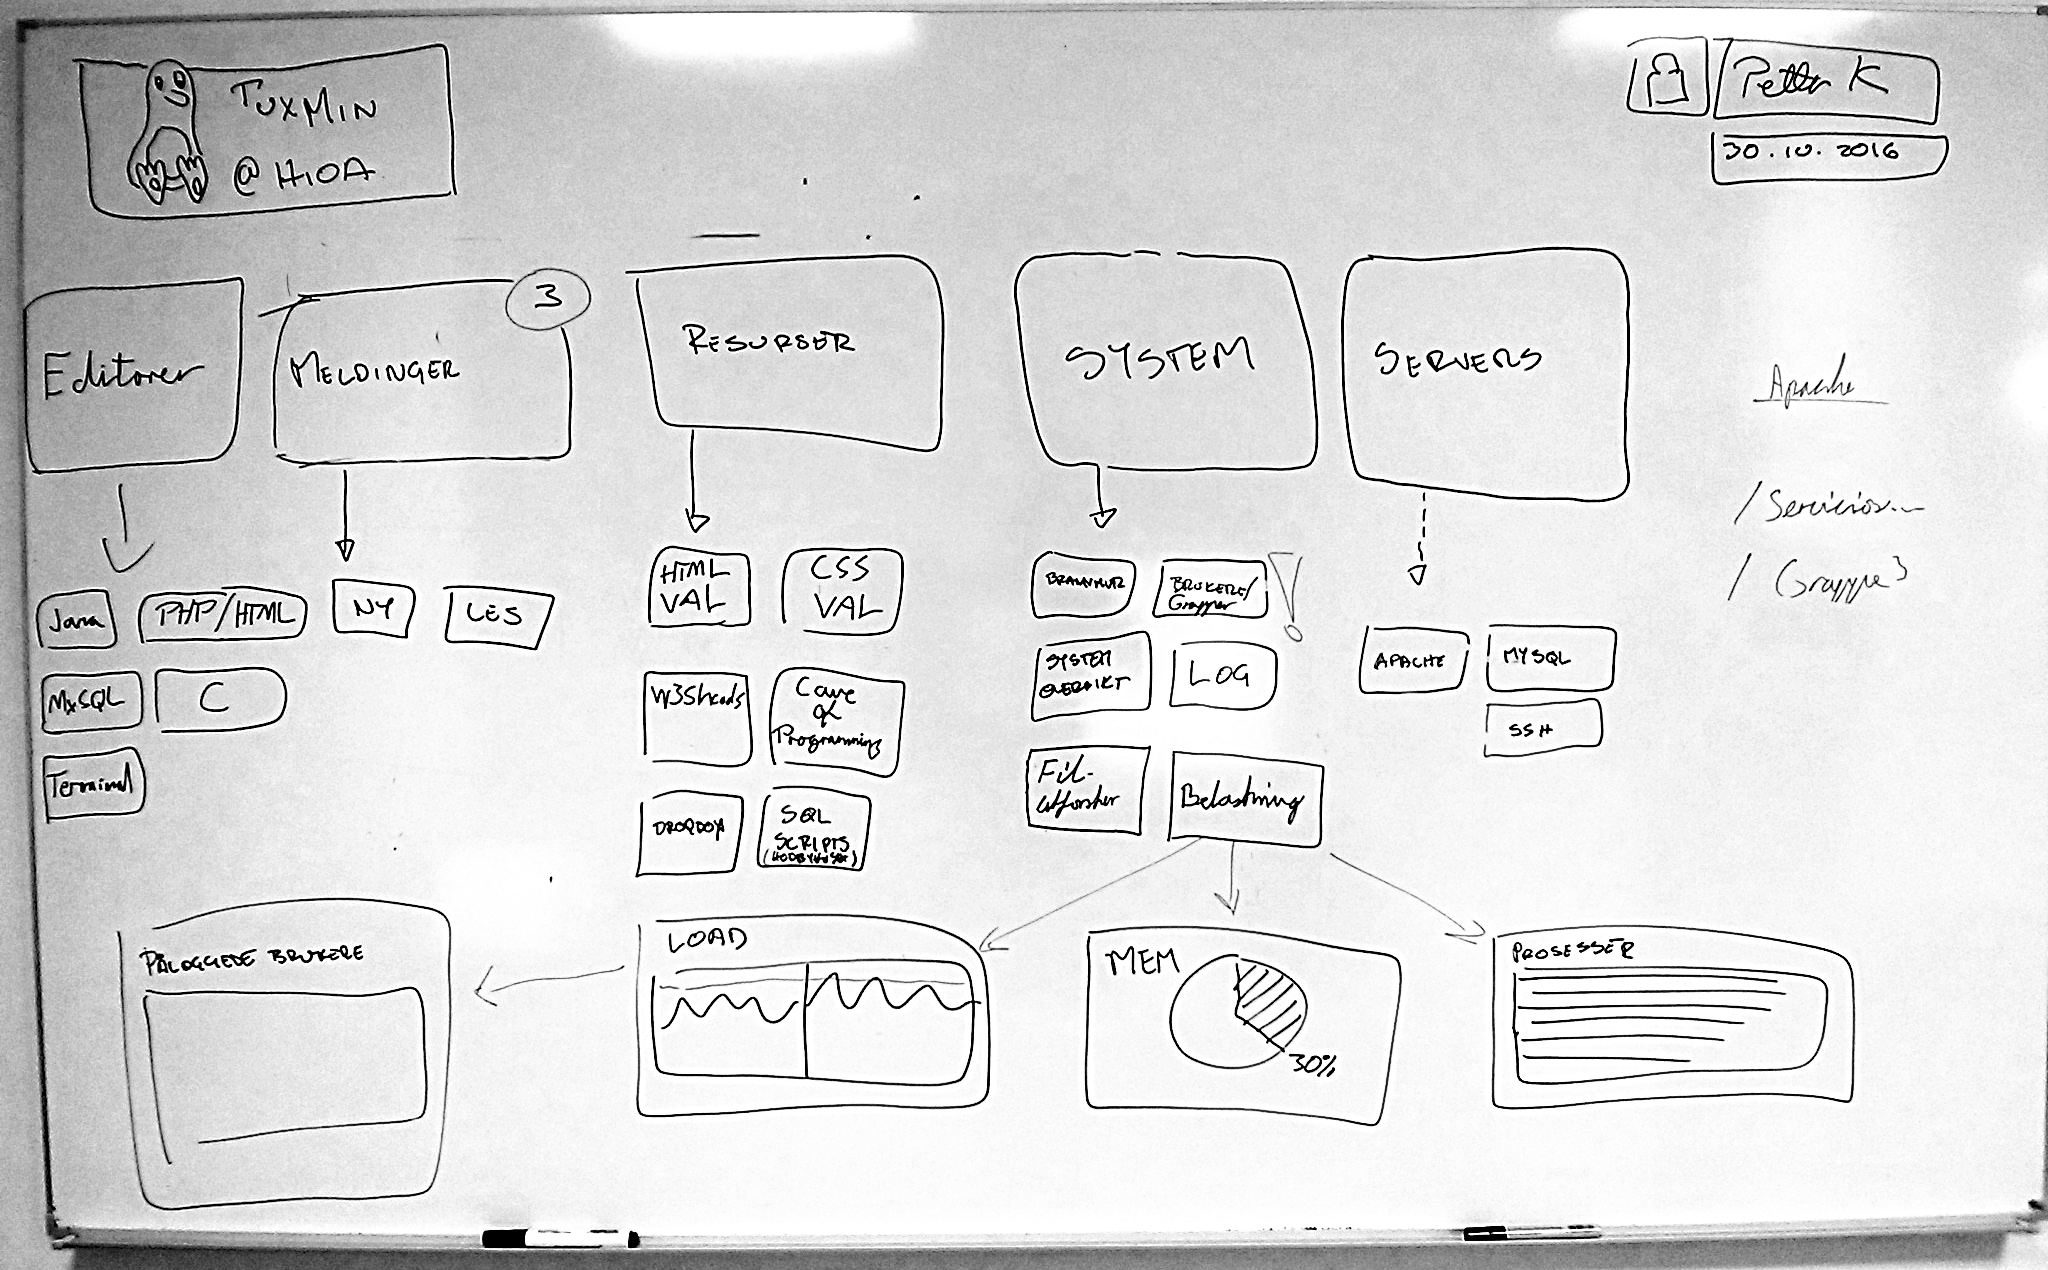
\includegraphics[width=\textwidth,height=\textheight,keepaspectratio]{./img/prosessdokumentasjon/foersteutkast/foerste.jpg}
\caption[Første utkast]{Første utkast over brukergrensesnittet.}
\label{fig:foersteutkast}
\end{figure}

\section{Low-fi prototype}

\section{Hi-fi prototype}

\section{Kriterier og avgjøresler}
Fokuser på alle valg som ble tatt. Hvilke kriterier og 
prinsipper i faget ligger bak avgjørelsene? 

Her kan vi skrive om hvorfor vi har akkuratt valgt Linux. Hvorfor skal løsningen være webbasert og hvorfor skal den kjøres i en virtuell maskin? Og så andre kriterier og avgjøresel som vi har tatt under veien. 
\chapter{Produktdokumentasjon}

\section{Pakker} \label{sec:klasserogpakker}
Da implementasjonen vi har lagt oss på krever mange javafiler, som ofte gjerne har relativt lite innhold har vi også delt javaklassene inn i flere pakker under mappen “src”.

\subsection*{\texttt{controller}}
Controller og undermappen Registrer inneholder all funksjonalitet til alle JPanels, deres innhold og registreringsvinduer. Funksjonaliteten og nærmere beskrivelse av disse klassene finnes i andre deler av dokumentasjonen.

\subsection*{\texttt{lib}}
Lib er biblioteket av statiske metoder, konstanter og enum, samt andre klasser og metoder som ikke naturlig hører til MVC-tankegangen.
Her finnes også våres RegEx-konstanter som er brukt på alle Tekstfelt i GUI, samt på nytt i kontrollerne. Det testes altså to ganger, før registrering og validering før objektet opprettes/endres.

\subsection*{\texttt{model} og \texttt{register}}
Model inneholder klassene det lages objekter av, som igjen legges inn i datasettene. Klassene Person og Bolig er abstrakte med hver sine subklasser. Klassen TabellModell er en abstrakt klasse som arver DefaultTableModel, og den har igjen klasser som arver dens funksjonalitet. Dette vil en kunne lese mer om i beskrivelsen av tabellimplementasjonen.
Pakken Register inneholder tomme klasser. Hensikten med å ha egne registerklasser, ut over det å ha alle HashSett i MainController er å implementere serializable. Det er altså disse klassene som serialiseres, og som inneholder alle datasett som blir skrevet til og lest fra fil.

\subsection*{\texttt{search}}
Search inneholder filene for søkeimplementasjonen vi har utviklet. Dette er en helt egenutviklet løsning som vil bli beskrevet nærmere i avsnittet for søkeimplementasjonen \ref{sec:sok}, side \pageref{sec:sok}.

\subsection*{\texttt{serviciosdevivienda}}
Det er to klasser her. Mainmetoden vår, serviciosdevivienda.java, samt SkrivTilLesFraFil.java som utfører all serialisering av data. Serialisering blir dokumentert nærmere her \ref{sec:serialisering}, side \pageref{sec:serialisering}.

\subsection*{\texttt{view} og undermappen \texttt{registrer}}
Disse to pakkene inneholder alle brukergrensesnitt, egendefinerte javakomponenter som \emph{CustomJTextField, CustomSubPanel} osv.
Det er brukt en stor mengde kreativitet og tankevirksomhet for å komme frem til løsningen vi har endt opp med, og det vil blir beskrevet flere andre steder i rapporten.



\section{Start og avslutting}
Programstart foretas fra pakke \texttt{ServiciosDeVivienda} fra en main metode med samme navn. Programmet blir startet med bruk av \texttt{SwingUtilities} hvilket gjør det mulig at \texttt{Swing} komponentene blir startet i en "<trygg"> programtråd som et tilpasset for bruk med \texttt{Swing} klassen (se ekespel \ref{kode:oppstart1}). Med slik tilnærmingsmåte forventes det at GUI delen av programmet skal bli mer stabilt. 

Programmet blir også avsluttet med hjelp av \texttt{ShutDownHook} på en måte som er anbefalt for \texttt{JVM}. Løsningen gir en mulighet til å avslutte programmet på en "<naturlig"> måte slik at eventuelle alle konkurrerende tråder får kjøre parallelt frem til avslutting. Løsningen sikrer at data som blir serialisert og skrevet til fil med mindre sjanse for feil og eventuelle skrive og lese feil.

\begin{lstlisting}[caption=Oppstart av programmet., label=kode:oppstart1]
		//Start
        SwingUtilities.invokeLater(new Runnable() {

            SkrivTilLesFraFil startProgram;

            @Override
            public void run() {
                startProgram = new SkrivTilLesFraFil();
                //Avslutting
                Runtime.getRuntime().addShutdownHook(new Thread(new Runnable() {
                    @Override
                    public void run() {
                        System.out.println("Programmet avsluttes");
                        startProgram.lagreData();
                    }
                }));
            }
        });
\end{lstlisting}
\section{Serialisering} \label{sec:serialisering}
Skriving og innlesing av data blir kalt opp fra programmets \texttt{main} metode. Les og skrive metoder finnes i \texttt{SkrivTilLesFraFil.java}. Den klassen initierer \texttt{MainController.java} som er programmet primære kontroller i MVC arkitekturen. Alle registre blir initialisert fra les/skrive klassen med hensikt å ha mulighet til å seriasliere alle registrene på plass. 
Eksempel \ref{kode:ser1} viser hvordan registrene og static variabler blir håndtert ved skrivning og serialisering. 
Programmets arkitektur baserer seg på tellevariabler som holder kontroll på antall objekter som til hver gang blir opprettet og lagt til i hvert enkelt register. Statiske filer blir skrevet i spesifikk rekkefølge etter at alle registrene (\texttt{HashSet}) er skrevet til fil.
Ved innlesing av lagret data blir alle registrene passert som komponenter til \texttt{MainKontroller}, se eksempel \ref{kode:ser2}. 

Lesing og skriving er opprettet etter \texttt{Java SE 6} struktur, derfor benytter vi oss ikke av  "<try-med resurser"> tilnærming. Hensikt med den brukte løsningen er at det oppleves som at vi får en mer oversiktlig kode.


\begin{lstlisting}[caption=Serialisering og skriving av data.,label=kode:ser1]
    public void lagreData() {
        try {
            FileOutputStream fos = new FileOutputStream(new File(Konstanter.FILNANV));
            ObjectOutputStream out = new ObjectOutputStream(fos);

            out.writeObject(personliste);
            out.writeObject(boligliste);
            out.writeObject(annonseliste);
            out.writeObject(kontraktliste);
            out.writeObject(soknadsliste);

            out.writeInt(Person.getTeller());
            out.writeInt(Bolig.getTeller());
            out.writeInt(Annonse.getTeller());
            out.writeInt(Soknad.getTeller());
            out.writeInt(Kontrakt.getTeller());

            out.close();

        } catch (IOException e) {
            System.out.println(e.fillInStackTrace());
        }
    }
\end{lstlisting}

\begin{lstlisting}[caption=Innlesing av serialisert data.,label=kode:ser2]
    public void lesInnData() {
        try {
            FileInputStream fis = new FileInputStream(new File(Konstanter.FILNANV));
            ObjectInputStream in = new ObjectInputStream(fis);

            personliste = (HashSet<Person>) in.readObject();
            boligliste = (HashSet<Bolig>) in.readObject();
            annonseliste = (HashSet<Annonse>) in.readObject();
            kontraktliste = (HashSet<Kontrakt>) in.readObject();
            soknadsliste = (HashSet<Soknad>) in.readObject();

            Person.setTeller(in.readInt());
            Bolig.setTeller(in.readInt());
            Annonse.setTeller(in.readInt());
            Soknad.setTeller(in.readInt());
            Kontrakt.setTeller(in.readInt());

            in.close();
            mainController = new MainController(personliste, boligliste, annonseliste, kontraktliste, soknadsliste);

        } catch (IOException e) {
            System.out.println(e.fillInStackTrace());

        } catch (ClassNotFoundException e) {
            System.out.println(e.fillInStackTrace());
        }
    }
\end{lstlisting}
\section{MVC}
Programmeringskonseptet \texttt{Model View Controller} er noe vi så vidt har vært gjennom i pensum, men om helt klart var noe av det første vi bestemte oss for å ta i bruk.
Et hvert dataprogram står i fare for å ende opp med enormt store GUI-klasser om man ikke gjør noen grep. I tillegg vil all kode være eksklusiv for den klassen og ikke kunne gjenbrukes fra andre klasser. Har man to-tre vinduer som skal utføre omtrent samme type oppgaver ender man opp med å skrive omtrent identisk kode for både brukergrensesnittet og funksjonaliteten flere ganger.
Man står også i fare for veldig omstendelig kode som er vanskelig å vedlikeholde, og som gjør videre utvikling og utvidelse av funksjonalitet betraktelig vanskeligere.

\subsection{Generelt om den strukturelle oppbyggingen}
Da boligsøkere har behov for å søke etter boliger trenger de både et søkepanel, en tabell eller listevisning av søkeresultatene og en visning av de enkelt annonseobjektene.
Vi la også merke til at megler ville ha omtrent det samme behovet, bare med mulighet for å behandle boliger, personer, søknader og kontrakter i tillegg.

Derfor har vi valgt å løse ved å lage to "versjoner" av samme brukergrensesnitt og kontrollerfunksjonalitet.
Det vil si en \texttt{Layout} basert på \texttt{BorderLayout} med et søkepanel på på toppen, en tabell på venstreside, et resultatvindu i sentrum og et knappepanel i bunnen.
Vi har dermed endt opp med en ramme av \texttt{toppPanel, venstrePanel, senterPanel} og \texttt{bunnPanel} som i sin tur tar inn paneler i form av egne klasser. På denne måten har vi kunnet lage to versjoner av \texttt{toppPanel}, én for \texttt{meglerVindu} og én for \texttt{annonseVindu}. De andre panelene er felles for begge visningene, men kunne selvsagt byttes ut eller deles opp på tilsvarende måte relativt enkelt og raskt.

I de følgende delkapitlene vil det gås nærmere inn på hvordan de forskjellige programmeringslagene henger sammen og jobber seg i mellom.

\subsection{Oppstart av kontrollere og brukergrensesnitt}
Den første klassen som instansieres fra \texttt{SkrivtilLesFraFil.java} under oppstart er \texttt{MainController.java}.
Det er fra denne kontrolleren alt annet starter, og det er her programmet "<deler"> seg i tre. 
Denne kontrolleren har da det overordnede ansvar for å holde programmet sammen, og har da tilgang til alle relevante kontrollere, brukergrensesnitt og datasett. 
Ut over å starte opp brukergrensesnitter og kontrollerne finnes det noen implementasjoner av spesialsydde "<\texttt{lyttere}">. 
Da alle våre paneler er egne javaklasser og søkeknappen i \texttt{toppPanel} skal returnere et datasett til \texttt{venstrePanel} sin tabell, så har vi laget \texttt{interface} som kontrolleres fra \texttt{MainController.java}. Skjer det en endring i \texttt{toppPanel}, nærmere bestemt i \texttt{ActionPerformed}-metoden, så sendes søkeresultatet via \texttt{MainController.java} til \texttt{venstrePanel} sine tabell-metoder. Dette helt uten at kontrollerne for de to panelene vet om hverandre.
Bruken av slike lyttere er brukt flere steder i programmet og vil bli dekket, med eksempler her \ref{sec:kontrollerlyttere} på side \pageref{sec:kontrollerlyttere}.

Når alle kontrollere er instansiert og brukergrensesnittet opprettet så kjøres det to metoder som setter opp flere \texttt{lyttere} i \texttt{ControllerTabell.java}, samt sende et datasett til hvert av de vinduenes tabeller.



\newpage
\subsection{Oversikt over hvilken kontrollere som hører til hvilken GUI-klasse}


\begin{table}[ht]
\center
\caption{Oversikt over kontrollerne og deres tilhørende GUI-klasser}
\label{tab:kontrollerguikobling}
\begin{tabular}{|l|l|}

\hline
Kontroller						& GUI-klasse \\ \hline

ControllerBildeViser.java		& BildeViser.java \\
ControllerBunnPanel.java			& BunnPanel.java \\
ControllerKeyBindings.java		& \\
ControllerOutput.java			& SenterPanel.java \\
ControllerTabell.java			& VenstrePanel.java \\
ControllerToppPanelMegler.java	& TopPanelMegler.java \\
ControllerToppPanelAnnonse.java  & TopPanelAnnonse.java \\
Innloggingskontroller.java		& LoggInnDialog.java \\
MainController.java				& \\
ControllerRegistrerAnnonse.java  & AnnonseRegVindu.java \\
ControllerRegistrerBolig.java 	& BoligRegVindu.java \\
ControllerRegistrerLeietaker.java 	& PersonRegVindu.java \\
ControllerRegistrerSoknad.java 	& SoknadRegVindu.java \\
ControllerRegistrerUtleier.java 	& PersonRegVindu.java \\


\hline
\end{tabular}
\end{table}
\section{Datastruktur \texttt{(Model)}} \label{sec:Datastruktur}

\subsection{Valg av datastruktur}
Alle dataregistrene er laget på \texttt{HashSet} fra \texttt{Collection}-rammeverket til \texttt{Java}. Vi har brukt \texttt{HashSet} for å unngå dobbellagring av like objekter. Vi har "<overridet"> \texttt{equals} og \texttt{hashcode}-metodene for objektene slik at de bare relevante datafelter brukes for å identifisere hva som er et unikt objekt og ikke. For eksempel så er det autoinkrementerte ID-feltet som gir alle objekter en unik ID, utelatt fra \texttt{equals} og \texttt{hashcode} da alle objekter da ville bli oppfattt som unike objekter.
Videre har vi ikke hatt bruk for sortering av dataene våre. Alle datasett blir sortert når de vises i tabellen.

I pakken \texttt{register} ligger selve registerne som igjen inneholder hver sitt \texttt{HashSet}. Alle registerklassene arver \texttt{Register.java} som har en del generiske metoder som fungerer på alle \texttt{HashSettene} og deres objekter.

\subsection{Datatyper}
Alle objektene, \texttt{Person, Bolig, Annonse, Søknad}, og \texttt{Kontrakt} har hver sin statiske teller som tildeles hvert objekt som opprettes. Bolig-objektene har teller fra 20000 til 29999. Annonse fra 30000 til 39999 osv.
Alle objektklassene implementerer \texttt{interfacet Searchable} som vi har utviklet selv. dette \texttt{interfacet} har en metode som heter \texttt{toString} som returnerer et \texttt{array av String-elementer}. Denne metoden definerer hva som skal inngå i fritekstsøket som beskrives mer her \ref{sec:sok} på side \pageref{sec:sok}.

\subsubsection{Bolig}
Klassen \texttt{Bolig.java} er \texttt{abstrakt} og har to subklasser; \texttt{Leilighet} og \texttt{Enebolig}. Grunnet begrensning i tid har vi ikke valgt å implementere flere typer boliger enn dette.
Boligobjektene har også en variabel \texttt{erUtleid}. Om en bolig er utleid vil ikke den kunne slettes fra datasettet \texttt{boligliste}.
Det er også en variabel som definerer en filsti til bilder av boligen. Informasjon om denne funksjonaliteten kan man lese mer om her \ref{sec:bilder}.

\subsubsection{Person}
Klassen \texttt{Person.java} er abstrakt og har som \texttt{Bolig.java} også subklasser; \texttt{Utleier.java, Leietaker.java} og \texttt{Megler.java}.
Det er ikke implementert all funksjonalitet man gjerne skulle ønske seg på disse klassene. Megler-klassen har ikke noe registreringsvindu. Det er hardkodet en megler for å kunne vise funksjonaliteten med pålogging til \texttt{meglerVindu}, men det er lagt større vekt på å få \texttt{Leietaker} og \texttt{Utleier} godt implementert da det er disse som skal behandles i annonser, søknader osv.

\subsubsection{Annonse}
Annonseobjektet består i hovedsak av et Bolig-objekt pluss noen egne felter for utleierpris, depositum, utleiers krav til leietaker osv.
Det er her også noen \texttt{Calendar}-variable som er tiltenkt bruk ved fremtidig utvidelse av programmet. Metoder \texttt{datoAnnonseRegistrert} og \texttt{datoAnnonseTasAvNett} vil kunne gi megler veldig mange muligheter for å lage statistikk på hvor lenger en annonse har vært på nett før den leies ut osv. 

\subsubsection{Søknad}
En søknad består av et annonseobjekt, leietakerobjekt, søknadsID og to \texttt{boolske} variabler for om søknaden er behandlet og godkjent.
Det er lagt opp til at mange søknader på samme annonse kan havne i megler sin liste over innkomne søknader. Søknadene sorteres da først synkende på kolonnen \texttt{erBehandlet}, og så stigende på kolonnen \texttt{annonseID}.
I det én søknad blir godkjent av megler så vil alle andre søknader automatisk bli markert som "behandlet" og som "ikke godkjent". 
Det er foreløpig ikke implementert en tilbakemeldingsfunksjon til boligsøkerne om deres søknader er godkjent eller avslått, men det ligger det selvfølgelig til rette for.

\subsubsection{Kontrakt}
En Kontrakt opprettes automatisk i det en søknad godkjennes. Annonseobjektet, Meglerobjektet og Leietakerobjektet, samt info om leiepris, depositum og dato kontrakten ble inngått er hoveddelene i kontrakten, og denne informasjonen kan ikke slettes eller endres. 
Optimalt sett skulle vi hatt en utskriftsvennlig versjon av en slik kontrakt, men det er ikke funnet tid til dette. 



\section{Brukergrensesnitt \texttt{(View)}} \label{sec:brukergrensesnitt}

Dette delkapittelet er litt overlappende med kapittelet "Swing-komponenter". Les gjerne mer om det her \ref{sec:swing} \pageref{sec:swing}.

\subsection{Oppstart av brukergrensesnittet}
I \texttt{MainController.java} instansieres først to arkfaner, \texttt{ArkfaneMegler.java} og \texttt{ArkfaneAnnonse.java}.
Disse sendes så med som parametere inn i strukturen til brukergrensesnittet, først til \texttt{StartGUI.java}, og så videre til \texttt{MainPanel.java} som oppretter \texttt{JTabbedPane} og legger inn de to arkfanene der.
Grunnen til at arkfanene ble opprettet allerede i \texttt{MainController.java} er fordi vi sender med det respektive arkfane under instansiering av \texttt{kontrollerne}. 
Siden de to arkfanene har så lik funksjonalitet, deler de på \texttt{kontrollerne} som de har felles.

Fra \texttt{MainController.java} opprettes det to versjoner av \texttt{ControllerTabell.java}. Til den ene sendes vinduet \texttt{meglerVindu} som er instans av \texttt{ArkfaneMegler.java} og til den andre kontrollerinstansen sendes \texttt{annonseVindu} som er instans av \texttt{ArkfaneAnnonse.java}.
Se figur \ref{fig:maincont}.

\begin{figure}[ht]
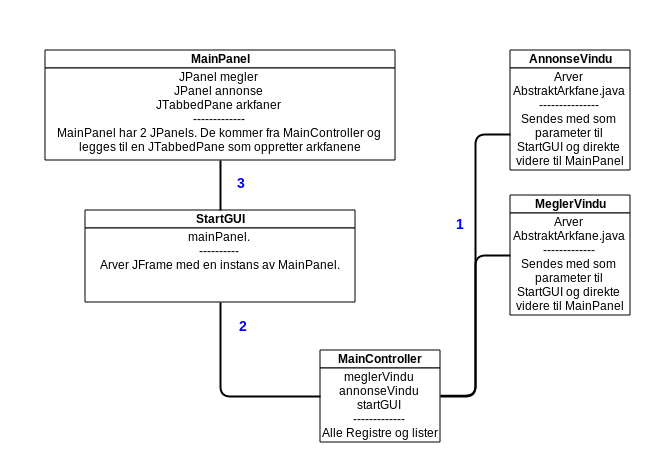
\includegraphics[width=\textwidth,height=\textheight,keepaspectratio]{./img/produktdokumentasjon/bilder/Controller_og_GUI-opprettelse2.png}
\caption[\texttt{MainController}: Programmoppstart]{Illustrasjon over hvordan \texttt{MainController} starter opp programmet}
label{fig:maincont}
\end{figure}


\subsection{Bruk av arv i brukergrensesnittet}
Brukergrensesnitt er utrolig tidskrevende å jobbe med, mye av det man gjør er å skrive samme kode for hvert enkelt vindu.
For å unngå dette mest mulig, samt å få alle vinduer og paneler til å ha mest mulig den samme følelsen har vi noen abstrakte klasser som vi arver på tvers av alle klassene som har med brukergrensesnitt å gjøre.


\subsubsection*{\texttt{AbstractPanel.java}}
Dette panelet arver \texttt{JPanel} og er superklassen til alle andre hovedvinduer og paneler i programmet, klassen inneholder to \texttt{konstruktører}. Den ene tar inn to heltall som representerer bredde og høyde på det panelet som arver klassen, samt en \texttt{String borderTitle} som blir tittel på kantlinjen som \texttt{konstruktøren} oppretter.
Den andre \texttt{konstruktøren} er omtrent lik, men tar ikke inn en \texttt{String} for kantlinje, så her kan man velge mellom to \texttt{konstruktører}, med eller uten kantlinje.
Dette panelet er også satt med en bakgrunnsfarge slik at alle paneler og vinduer som arver denne vil arve denne.

\texttt{CustomSubPanel.java} arver også \texttt{AbstractPanel.java}. Denne klassen brukes i hovedsak for paneler inne i et hovedpanel. Da dette panelet skal brukes gjentatte ganger i mange forskjellige sammenhenger er det hele 6 \texttt{konstruktører} her. 
I noen opprettes det en predefinert \texttt{Layout}, i andre ikke. Noen tar inn størrelse (bredde og høyde), andre ikke. På denne måten har vi fått en veldig slagkraftig klasse som har spart oss for mye arbeid og forenklet konstruksjonen av brukergrensesnitter veldig.


\subsubsection*{\texttt{AbstractRegistreringsVindu.java}, \texttt{AbstractRegistreringsPanel.java}}
\texttt{AbstractRegistreringsVindu.java} er superklassen for \texttt{AbstractRegistreringsPanel.java}. Denne klassen arver \texttt{JFrame} og er setter de mest generelle parameterne som et hvert vindu skal ha. Størrelse, navn på vinduet, samt standard lukkefunksjonalitet osv.
\texttt{AbstractRegistreringsPanel.java} er superklassen til alle registreringsvinduene. Denne klassen har en \texttt{BorderLayout} og tar inn parametere som bredde, høyde og tittel for vinduet som opprettes. Ut over dette gjør ikke denne klassen mye. Alle klasser som arver denne vil velge hvilke paneler fra denne klassens \texttt{BorderLayout} de ønsker å ta i bruk.


\subsection{Oppbyggningen av arkfanene}
Begge arkfanene er bygget over samme lest. De arver \texttt{AbstraktArkfane.java}. Denne klassen tar inn en \texttt{String} som avgjør hvilke \texttt{topPanel} som skal følge med arkfanen.
\texttt{AbstraktArkfane.java} består i korte trekk av en \texttt{BorderLayout} med fire paneler; \texttt{toppanel, venstrepanel, senterpanel} og \texttt{bunnpanel}.
Hvert av panelene er satt opp med en \texttt{get-metode} som brukes hyppig av \texttt{kontrollerne} i kommunikasjonen med komponentene der.

Alle \texttt{kontrollerne} er "<klar"> over sitt vindu, og nedenfor er et eksempel (\ref{kode:konttab}) på hvordan \texttt{ControllerTabell.java} kommuniserer med vinduet.

\begin{lstlisting}[caption={[\texttt{ControllerTabell.java}]\texttt{ControllerTabell.java} kommunikasjon med brukergrensesnitt.},label=kode:konttab]
        /**
         * Lytter på museklikk i Output-vinduet.
         */
        vindu.getSenterpanel().getEditorPane().addMouseListener(new MouseAdapter() {

            @Override
            public void mouseClicked(MouseEvent e) {
                if (e.getButton() == MouseEvent.BUTTON1) {
                    if (modellIBruk instanceof TabellModellAnnonse) {
                        Annonse valgtObjekt = returnerAnnonseObjekt();
                        if (vindu instanceof ArkfaneMegler) {
                            new ControllerBildeViser(valgtObjekt.getBolig(), true);
                        } else {
                            new ControllerBildeViser(valgtObjekt.getBolig(), false);
                        }
                    }
                }
            }

        });
\end{lstlisting}

I figuren ovenfor kan man både få tak i \texttt{vindu} sine paneler, men også teste om \texttt{vindu} er av type \texttt{ArkfaneMegler} eller ikke. Tidligere i prosjektet brukte vi \texttt{konstanter} som ble sendt med som parametere for å identifisere hvilke vindu man var i, og hvilken objekttype man behandlet til en hver tid.


\subsubsection*{\texttt{TopPanelMegler.java}, \texttt{TopPanelAnnonse.java}, \texttt{VenstrePanel.java}, \texttt{SenterPanel.java} og \texttt{BunnPanel.java}}
De tre nevnte panelene utgjør innholdet i hver av arkfanene. 
Da all funksjonalitet finnes i de respektive \texttt{kontrollerne} er hver av disse klassene ganske små. De består i grunn bare av en \texttt{Layout} samt den/de komponentene som vises, inkludert subpaneler samt \texttt{get-metoder} en trenger for å kunne hente informasjon derfra.
Det er brukt forskjellige \texttt{Layout-managere}, alt etter hvilken som er mest hensiktsmessig i den gitte situasjon.
I \texttt{VenstraPanel.java} og \texttt{SenterPanel.java} har man bare én komponent hver som dominerer hele panelet, men \texttt{kontrollerne} bak disse er desto større.
\texttt{JTable} i \texttt{VenstrePanel.java} har utrolig mye funksjonalitet og er hjerte i hele programmet.
\texttt{JEditorPane} i \texttt{SenterPanel.java} er en ren \texttt{output-pane} som skriver ut html-visning av objektene i tabellen. 


\subsection{Registreringsvinduene}
Registreringsvinduene er bygget over samme lest, og arver \texttt{AbstractRegistreringsPanel}. De er likevel ganske forskjellige. De bruker et utall forskjellige \texttt{Layout-managere}, og ofte en blanding mellom flere. 
\texttt{GridBagLayout} er allikevel den mest allsidige og foretrukne \texttt{Layout-manageren} vi har brukt. 

Så og si alle komponentene vi har brukt er \texttt{Custom..}. Det vil si egendefinerte komponenter vi har laget, og som arver den opprinnelige \texttt{Swing}-komponenten. 
Det beste eksempelet her er \texttt{CustomJTextField.java} som blant annet tar inn et \texttt{String pattern} som er en \texttt{RegEx}-konstant, slik at komponenten har innebygget \texttt{RegEx}-funksjonalitet.

Alle registreringsvinduene har i sine kontrollere egne konstruktører ment for nye objektet og for endring av objektene. Det vil si at når en endrer et objekt så fylles komponentene ut med relevant informasjon fra det innkomne objektet.

Når en velger ny \texttt{Bolig} eller har valgt et valg som gjelder bare for én type objekter så vil de valgene som ikke gjelder for det valget bli deaktivert og ikke mulig å legge inn informasjon på. Dette er selvfølgelig funksjonalitet som ligger i \texttt{kontrollerne} og vil bli nevnt i \ref{sec:regkontrollere} på side \pageref{sec:regkontrollere}.

Vi har gjort et eksperiment med \texttt{PersonRegVindu.java}. 
Dette er et felles registreringsvindu for både \texttt{Leietakere} og for \texttt{Utleiere}. Vinduet har to \texttt{kontrollere} som kaller på vinduet ved behov.
Dette betyr at en del komponenter vil være overflødige i noen tilfeller, og nødvendige i andre tilfeller. Dette vil bli nevnt mer i \ref{sec:regkontrollere} på side \pageref{sec:regkontrollere}.


\section{Kontroller \texttt{(Controller)}} \label{sec:kontroller}

\subsection{Generelt om kontrollermiljøet}
Da prosjektet startet var vi fornøyd med én \texttt{kontroller} og kalte den \texttt{MainController.java}. Det viste seg ganske raskt at den ville kunne bli enormt stor, så da endte vi opp med å dele den opp i flere deler. Siden den gang har vi besluttet at vi like godt kunne ha én \texttt{kontroller} til hvert vindu, og kanskje noen uten tilhørende vinduer også.
\texttt{MainController} instansierer alle \texttt{hovedkontrollerne}, bortsett fra \texttt{BunnController} som instansieres fra \texttt{ControllerTabell} og \texttt{ControllerOutput} som ikke instansieres. Den har bare statiske metoder som tar i mot diverse data og viser dem i \texttt{JEditorPane} formatert som \texttt{HTML}.

I tillegg til \texttt{hovedkontrollerne} har vi \texttt{registreringskontrollerne} som hører til hvert sitt registreringsvindu. De vil bli nevnt under \ref{sec:regkontrollere} på side \pageref{sec:regkontrollere}.

Det er et eget avsnitt i dette kapitelet vedrørende lyttefunksjonaliten vi har implementert for å kunne kommunisere mellom de forskjellige \texttt{kontrollerne} .

I den første delen av prosjektet var ikke \texttt{JTable}-implementasjonen vår veldig god og vi kunne ikke benytte oss av å teste hvilket datasett som var satt i tabellen. Dermed endte vi opp med å bruke identifikatorer for dette. Først med \texttt{konstanter} og så \texttt{Enum} som identifiserte personobjekter, boligobjektet osv.
Vi måtte derfor implementere \texttt{Interface}-lyttere som lyttet på når en ny \texttt{ArrayList} var satt i tabellen blant annet.

Siden det har tabellen kommet skikkelig på plass og det går nå an å teste hvilken type objekter som ligger i tabellen. Dermed har vi til dels begynt å teste på tabellens \texttt{getModel()}-metode for å finne instansen av datasettet.

Siden vi likevel er veldig  stolte av løsningen vår med \texttt{interface}-lyttere har vi valgt å beholde noe av implementasjonen og vil derfor ha et eget delkapittel for dette her \ref{sec:kontrollerlyttere}, på side \pageref{sec:kontrollerlyttere}.


\subsection{Hovedkontrollerne}
\texttt{Hovedkontrollerne} er betegnelsen på klassene:
\begin{itemize}[noitemsep,nolistsep]
\item \texttt{MainController.java} 
\item \texttt{ControllerTabell.java} 
\item \texttt{ControllerOutput.java}
\item \texttt{ControllerBunnPanel.java}
\item \texttt{ControllerToppPanelMegler.java} 
\item \texttt{ControllerToppPanelAnnonse.java}
\end{itemize}
Disse \texttt{kontrollerne} styrer absolutt all funksjonalitet mellom datastrukturen og brukergrensesnittet.


\subsection{\texttt{MainController.java}}
Denne klassen instansieres fra \texttt{SkrivTilLesFraFil.java}, der data blir lest inn fra fil og skrevet til fil.
Denne klassen har ikke noe brukergrensesnitt og den eneste oppgaven den har er å starte andre \texttt{kontrollere} og brukergrensesnittet.
I tillegg til det passer \texttt{kontrolleren} på at de andre komponentene som skal kommunisere sammen har mulighet til det. Dette er løst med en lytteløsning beskrevet her \ref{sec:kontrollerlyttere}, på side \pageref{sec:kontrollerlyttere}.


\subsection{\texttt{ControllerToppPanelMegler.java}}
Brukergrensesnittet til denne klassen gir megler mulighet til å søke i de forskjellige datasettene, samt registrere nye objekter.
I tillegg er det er enkelt statistikkpanel som viser antall ledige boliger og antall kontrakter signert i år.

Klassens primære funksjon er søkefunksjonaliteten og videresending av resultatet til tabellen.
Metoden \texttt{finnValgtObjektITabell} har en \texttt{ListSelectionListener} som lytter på tabellens \texttt{valueChanged}. Hver gang en ny rad er valgt i tabellen så returneres nummeret på raden som er valgt. Om verdien som returneres er forskjellig fra \texttt{-1} (når tabellen ikke har en valgt rad returneres -1) så konverteres nummeret til den bakenforliggende tabellmodellens index. Til slutt så lagres det et \texttt{Object valgtObjekt} som hentes på den indexen som er angitt.

Metoden \texttt{sendSokeResultat} tar i mot en streng fra søkefeltet, og avhengig av hvilken \texttt{radioknapp} som er valgt så kjøres søkemetoden på det rette datasettet. Resultatet lagres i en ArrayList. Søkemetoden er beskrevet nærmere her \ref{sec:sok}, på side \pageref{sec:sok}.
Resultatet blir så sendt ned til tabellen og vist der. Det skjer via \texttt{lytteren} som blir vist ved eksempel her \ref{sec:kontrollerlyttere}, på side \pageref{sec:kontrollerlyttere}.
Den private klassen \texttt{KnappeLytter} lytter på de fire knappene i brukergrensesnittet. Metodene tester på hvilken type objektet som er valgt i tabellen er og man får bare trykke på vedrørende knapp om det man ønsker å utføre er relevant.
Eksempelvis så skal man ikke kunne trykke på "Ny Bolig" uten å ha først valgt et personobjekt av typen \texttt{Utleier} i tabellen.

\subsection{\texttt{ControllerToppPanelAnnonse.java}}
Denne \texttt{kontrolleren} er mer avansert enn \texttt{ControllerToppPanelMegler.java}. Klassen benytter seg av et \texttt{AnnonseFilter} som er beskrevet i detalj her \ref{sec:annonsesok}, på side \pageref{sec:annonsesok}.
\texttt{Annonsefilteret} har to \texttt{get-metoder} som brukes for å fyllet ut de to \texttt{komboboksene} som lister boligtyper og poststeder. Det er metodene \texttt{addPoststederToComboBoxOnLoad} og \texttt{addBoligTyperToComboBoxOnLoad} som tar seg av denne jobben.
\texttt{Komboboksen} som lister opp poststed er implementert slik at den søker gjennom alle annonsene som er publisert og henter poststedet inn i listen. Det vil si at når én annonse forsvinner, så forsvinner også poststedet fra \texttt{komboboksen} også, så sant det ikke er andre annonser publisert for en bolig på samme poststed.

I det man trykker på søkeknappen i brukergrensesnittet så kjøres metoden \texttt{sendSokeResultat}. Denne metoden kjører så metoden \texttt{filtrerAnnonser}, og om \texttt{lytteren} er instansiert så sendes datasettet ned til tabellen via \texttt{interfacet} som står for kontakten mellom \texttt{kontrollerne}. Denne lyttefunksjonaliteten blir vist ved eksempel her \ref{sec:kontrollerlyttere}, på side \pageref{sec:kontrollerlyttere}.

Metoden \texttt{filtrerAnnonser} nevnt overnfor henter søkekriterier fra brukergrensesnittet og om kriteriene passerer RegEx-testen så sendes de med til \texttt{annonsefilteret} som parametere. Returen fra denne metoden er et \texttt{HashSet} av annonser.


\subsection{\texttt{ControllerBunnPanel.java}}
Denne klassen instansieres fra \texttt{ControllerTabell.java} i motsetning til de andre \texttt{kontrollerne}. Denne klassen har tre knapper som brukes i forbindelse med navigering i tabellen, samt til å åpne registreringsvinduet for valgt objekt for endring.
Klassen har én privat \texttt{KnappeLytter}-klasse som utgjør omtrent hele funksjonaliteten til denne \texttt{kontrolleren}.
Den ene knappen her har forskjellig funksjonalitet om man er i \texttt{annonseVindu} enn om man er i \texttt{meglerVindu}.
\texttt{Konstruktøren} til \texttt{KnappeLytteren} endrer navn på \texttt{MultiKnapp} som vi har valgt å kalle den. 
I \texttt{actionPerformed}-metoden vil det testes for hvilket datasett som ligger i tabellen, hvilken rad som er valgt, og hvilket vindu man befinner seg i. Se følgende eksempel \ref{kode:contbpan}:

\begin{lstlisting}[caption={[\texttt{ControllerBunnPanel.java}]Utdrag fra \texttt{actionPerformed}-metoden i \texttt{ControllerBunnPanel.java}}, label=kode:contbpan]
    if (tabell.getModel() instanceof TabellModellAnnonse) {
        modellIBruk = (TabellModellAnnonse) modellIBruk;
        if (vindu instanceof ArkfaneMegler) {
            new ControllerRegistrerAnnonse(annonseliste, personliste, (Annonse) modellIBruk.finnObjektIModell(valgtRad));
        } else {
            new ControllerRegistrerSoknad(personliste, annonseliste, soknadliste, (Annonse) modellIBruk.finnObjektIModell(valgtRad));
        }
    }
\end{lstlisting}

\subsection{\texttt{ControllerOutput.java}} \label{subsec:contout}
\texttt{SenterPanel.java} har én komponent som viser valgt objekt i tabellen i \texttt{HTML}visning. Alle metodene i denne klassen er statiske. De skal ikke behandle objekter, bare vise dem. Denne \texttt{kontrolleren} er derfor ikke instansiert noe sted.
Alle "<\texttt{HTML}-metodene"> tar i mot \texttt{JEditorPane}-komponenten det skal skrives til, i hvilket vindu man befinner seg i, objektet som skal vises og eventuelt et eller flere \texttt{HashSet} om en trenger ytterligere informasjon i utskriften.

\texttt{Utleier}-objekter har i visningen blant annet en liste over boliger de eier, om noen. Da er det hjelpemetoder som itererer over \texttt{boligregisteret} og finner eieren av hver \texttt{bolig}. \texttt{Boligene} til valgt valgt \texttt{Utleier} vil da returneres og skrives ut i \texttt{Utleier}-objektet.

Ut over selve metodene for å vise objekter så finnes metoden \texttt{setStylesheet} helt nederst i klassen.
Alle "<\texttt{HTML}-metodene"> må formateres så de passer inn i vinduet \texttt{JEditorPane} har tilgjengelig. 
Det er stort sett brukt tabeller for å vise objekter, og da \texttt{JEditorPane} ikke støtter nyere \texttt{HTML}-versjon enn 3.2 med \texttt{CSS} 1.0, så har vi vært ganske begrenset på hvor for seg gjort visningene kunne bli.
Det måtte en del justering på plass, da en ikke kan automatisk skalere bilder, som i nyere versjoner av \texttt{HTML}.


\subsection{\texttt{ControllerTabell.java}}
Denne \texttt{kontrolleren} er holder orden på alle data som skal vises i tabellen i \texttt{VenstrePanel.java} der tabellen ligger, samt funksjonalitet for å slette, endre og opprette nye objekter. \\
Dette kapittelet vil ta for seg noen nøkkelpunkter på funksjonalitet og flyt av data.

$\bullet$ Hvordan tabellen tar i mot data og settes opp, side \pageref{sec:oppsettabell} \\ 
$\bullet$ Datamodellene, sortering og formatering, side \pageref{sec:virkemåtetabell} \\
$\bullet$ PopupMeny-funksjonalitet, side \pageref{sec:interaktivitettabell} \\
$\bullet$ Lytter på klikk i Output-vinduet, side \pageref{sec:interaktivitettabell}


\subsubsection{Hvordan \texttt{kontrolleren} setter opp tabellen} \label{sec:oppsettabell}
I det programmet starter opp kaller \texttt{MainController.java} opp to metoder i \texttt{TabellController.java}, \texttt{settOppTabellLyttere} og \texttt{settInnDataITabell}.
Den første av disse tar for seg en hel del initialisering av tabellens virkemåte. Den andre tar i mot et datasett og setter det inn i tabellen. Den metoden vil bli beskrevet mer i avsnittet for tabellens virkemåte \ref{sec:virkemåtetabell}, side \pageref{sec:virkemåtetabell}.

En \texttt{JTable} har muligheter for utrolig mye funksjonalitet om en velger å ta det i bruk.
Vår implementasjon er for så vidt litt annerledes enn en del av eksemplene en kan lese om andre steder. Vi har valgt å ikke tillate endring i tabellen. En \texttt{JList} fant vi fort ut var for enkel, da vi gjerne også ville kunne sortere på kolonner.

I prosessen har vi endret tabellens datastruktur to ganger. Først ble det blant annet brukt en \texttt{array}, men da den er vanskelig å slette fra uten mye ekstra prosessering så endte vi opp med en \texttt{ArrayList} som datastruktur. Da vår tabell skal liste ett objekt per linje, så valgte vi ikke å bruke en flerdimensjonal \texttt{array}. 

Metoden \texttt{settOppTabellLyttere} gjør litt mer enn bare å sette opp \texttt{lyttere}. Først initialiserer den \texttt{ControllerBunnPanel.java} sin private \texttt{lytteklasse}.
Videre kalles metoden \texttt{settOpplyttereForPopupMenyITabell} som definerer funksjonaliteten til \texttt{PopupMenu} når en høyreklikker i tabellen. Les mer om den på \ref{sec:interaktivitettabell}, på side \pageref{sec:interaktivitettabell}.
Metoden kobler så tabellen og popupmenyen sammen via tabellens \texttt{setComponentPopUpMenu}-metode, før den initialiserer slettefunksjonalitet i tabellen når en bruker \texttt{Delete}-knappen på tastaturet. Se følgende eksempel (\ref{kode:slett1}):
\begin{lstlisting}[caption=Slettefunksjonalitet i tabellen ved å trykke Delete på tastaturet.,label=kode:slett1]
        inputMap = tabell.getInputMap(JTable.WHEN_FOCUSED);
        actionMap = tabell.getActionMap();

        Action sletteknappFunksjon = new AbstractAction() {
            @Override
            public void actionPerformed(ActionEvent e) {
                generellSletteMetodeSomKallerOppRettSletteMetode();
            }
        };

        inputMap.put(KeyStroke.getKeyStroke(KeyEvent.VK_DELETE, 0), "Slett");
        inputMap.put(KeyStroke.getKeyStroke(KeyEvent.VK_BACK_SPACE, 0), "Slett");
        actionMap.put("Slett", sletteknappFunksjon);
\end{lstlisting}


Metoden som kalles opp \texttt{generellSletteMetodeSomKallerOppRettSletteMetode} kaller igjen på den rette metoden som faktisk utfører slettingen. Det er tre slettemetoder i \texttt{kontrolleren}; \texttt{slettPerson, slettBolig} og \texttt{slettAnnonse}.

Metoden er nå kommet for å initialisere diverse lyttere. De vil vises med eksempler. Først ut er tabellens funksjonalitet for å oppfatte hvilken rad som er valgt, og deretter kalle på metoden \texttt{sendObjektFraTabellTilOutput}. Det vil si at hver gang en ny linje velges i tabellen så kjøres denne \texttt{sendObjektFraTabellTilOutput}-metoden, som plukker opp hvilken type objekt som er valgt og sende det til output-vinduet. Se følgende eksempel (\ref{kode:lytt1}):
\begin{lstlisting}[caption=Lytteren som finner valgt rad i tabellen.,label=kode:lytt1]
        tabell.getSelectionModel().addListSelectionListener(new ListSelectionListener() {

            @Override
            public void valueChanged(ListSelectionEvent e) {

                if (e.getValueIsAdjusting()) {
                    return;
                }
                try {
                    int rad = tabell.getSelectedRow();
                    if (rad > -1) {
                        rad = tabell.convertRowIndexToModel(rad);

                        //Lagrer raden i en variabel, som brukes i andre metoder.
                        valgtRadItabell = rad;
                        sendObjektFraTabellTilOutput(objekttype);
                    }

                } catch (ArrayIndexOutOfBoundsException aiobe) {
                    System.out.println("Tabell ConvertRowIndexToModel ArrayIndexOufOfBounds");
                } catch (IndexOutOfBoundsException iobe) {
                    System.out.println("Tabell ConvertRowIndexToModel IndexOufOfBounds");
                }
            }
        });
\end{lstlisting}

De resterende \texttt{lytterne} vil bli dekket i avsnittet om interaktivitet i tabellen \ref{sec:interaktivitettabell}, på side \pageref{sec:interaktivitettabell}.


\subsubsection{Tabellens oppsett, virkemåte og formatering} \label{sec:virkemåtetabell}

En \texttt{JTable} kan implementeres på forskjellige måter. Ofte holder det med å implementere en \texttt{DefaultTableModel}, men i vårt tilfelle der vi har forskjellige typer objekter som krever forskjellige kolonnenavn så har vi valgt å la klassen \texttt{TabellModell.java} arve \texttt{DefaultTableModel} og override de metodene vi har behov for. Videre så vil subklassene til \texttt{TabellModell.java}, som \texttt{TabellModellAnnonse.java} spesifisere hvilke kolonnenavn man har i det datasettet, samt hvilke felter i et annonseobjekt som skal hentes til hvilken kolonne. 

Klassen \texttt{VenstrePanel.java} hvor tabellen instansieres er også der man finner noe av tabellens utvidete funksjonalitet.

Metoden \texttt{settCelleRenderer} definerer hvordan spesifikke celler i tabellen skal formateres. Her er det bare definert én regel og det er for behandlede \texttt{Søknadsobjekter}. Metoden finner ut hvilken \texttt{TabellModell} som er i bruk, og så tester den kolonnen "<Er behandlet"> (nummer 2) i \texttt{TabellModellAnnonse.java} om søknaden er behandlet eller ikke. er den behandlet skal cellen "dimmes" ned. Metoden gjengis i sin helhet i eksempel \ref{kode:cellerend1} under:
\begin{lstlisting}[caption=Metoden \texttt{settCelleRenderer} fra \texttt{VenstrePanel.java}.,label=kode:cellerend1]
    public void settCelleRenderer() {

        tabell.setDefaultRenderer(Object.class, new DefaultTableCellRenderer() {
            @Override
            public Component getTableCellRendererComponent(JTable tabell, Object verdi, boolean erValgt, boolean harFokus, int rad, int kolonne) {
                TabellModell modell = (TabellModell) tabell.getModel();

                Component c = super.getTableCellRendererComponent(tabell, verdi, erValgt, harFokus, rad, kolonne);
                if (modell instanceof TabellModellSoknad) {
                    if (tabell.getValueAt(rad, 2).equals("Ja")) {
                        c.setForeground(new Color(200, 200, 200));
                    } else {
                        c.setForeground(Color.BLACK);
                    }
                }
                c.repaint();
                return c;
            }
        });

    }//End method
\end{lstlisting}

Metoden \texttt{resizeKolonneBredde} kalles opp hver gang et nytt datasett er lagt inn i tabellens modell. Metoden består av to \texttt{for}-løkker inne i hverandre som itererer gjennom alle cellene i tabellen. For hver kolonne så finner metoden den cellen som "bruker mest plass" og setter kolonnebredden til det.
Metoden er gjengitt i sin helhet i eksempel \ref{kode:resize1} under:
\begin{lstlisting}[caption=Metoden \texttt{resizeKolonneBredde} fra klassen \texttt{VenstrePanel.java},label=kode:resize1]
    public void resizeKolonneBredde() {
        TableColumnModel kolonneModell = tabell.getColumnModel();
        Component comp = null;
        TableCellRenderer renderer = null;

        for (int kol = 0; kol < tabell.getColumnCount(); kol++) {
            int bredde = 50; //minste bredde
            for (int rad = 0; rad < tabell.getRowCount(); rad++) {
                renderer = tabell.getCellRenderer(rad, kol);
                comp = tabell.prepareRenderer(renderer, rad, kol);
                bredde = Math.max(comp.getPreferredSize().width, bredde);
            }
            kolonneModell.getColumn(kol).setPreferredWidth(bredde);
        }
    }
\end{lstlisting}

Metoden \texttt{sorterTabellVedOppstart} definerer en sorteringsrekkefølge på tabellens første kolonne, slik at tabellen alltid er sortert på ID-feltet til gjeldene objekt.
Metoden \texttt{sorterTabellSoknadData} gjelder bare for \texttt{Søknadobjekter} i \texttt{TabellModellSoknad.java}. Denne sorterer først synkende på kolonnen "Er behandlet", og deretter på ID-kolonnen. Man vil da alltid ha ubehandlede søknader liggende øverst i tabellen, sortert innad på AnnonseID. 

Hvilken av disse sorteringsmetodene som tas i bruk bestemmes metoden \texttt{settInnDataITabell} i \texttt{ControllerTabell.java}.
Metoden tar inn et datasett i form av \texttt{HashSet} eller \texttt{ArrayList}, samt en \texttt{Enum}-variabel som identifiserer hvilken \texttt{radioknapp} som er valgt i søkepanelet i enten \texttt{TopPanelMegler.java} eller \texttt{TopPanelAnnonse.java}. Metoden har en \texttt{switch/case} på \texttt{Enum}-variabelen og utfører så de instuksjoner som er gjeldende for det datasettet som skal inn i tabellen.
Hele metoden er gjengitt i eksempel \ref{kode:settinn1}:
\begin{lstlisting}[caption=Metoden \texttt{settInnDataITabell} i \texttt{ControllerTabell.java},label=kode:settinn1]
    public void settInnDataITabell(Collection innkommendeDatasett, ObjektType objekttypeEnum) {

        if (innkommendeDatasett.size() > 0) {
            tabellData = new ArrayList<>();
            Iterator<?> iter = innkommendeDatasett.iterator();
            while (iter.hasNext()) {
                tabellData.add(iter.next());
            }

            try {
                switch (objekttypeEnum) {
                    case PERSONOBJ:
                        this.objekttype = ObjektType.PERSONOBJ;
                        tabellModellPerson.fyllTabellMedInnhold(tabellData);
                        tabell.setModel(tabellModellPerson);
                        tabellModellPerson.fireTableStructureChanged();
                        modellIBruk = tabellModellPerson;
                        vindu.getVenstrepanel().sorterTabellVedOppstart();
                        break;
                    case BOLIGOBJ:
                        this.objekttype = ObjektType.BOLIGOBJ;
                        tabellModellBolig.fyllTabellMedInnhold(tabellData);
                        tabell.setModel(tabellModellBolig);
                        tabellModellBolig.fireTableStructureChanged();
                        modellIBruk = tabellModellBolig;
                        vindu.getVenstrepanel().sorterTabellVedOppstart();
                        break;
                    case ANNONSEOBJ:
                        this.objekttype = ObjektType.ANNONSEOBJ;
                        tabellModellAnnonse.fyllTabellMedInnhold(tabellData);
                        tabell.setModel(tabellModellAnnonse);
                        tabellModellAnnonse.fireTableStructureChanged();
                        tabell.getColumnModel().getColumn(2).setCellRenderer(vindu.getVenstrepanel().settHoyrestilltFormateringPaaTabell());
                        tabell.getColumnModel().getColumn(3).setCellRenderer(vindu.getVenstrepanel().settHoyrestilltFormateringPaaTabell());
                        modellIBruk = tabellModellAnnonse;
                        vindu.getVenstrepanel().sorterTabellVedOppstart();
                        break;
                    case KONTRAKTOBJ:
                        this.objekttype = ObjektType.KONTRAKTOBJ;
                        tabellModellKontrakt.fyllTabellMedInnhold(tabellData);
                        tabell.setModel(tabellModellKontrakt);
                        tabellModellKontrakt.fireTableStructureChanged();
                        modellIBruk = tabellModellKontrakt;
                        vindu.getVenstrepanel().sorterTabellVedOppstart();
                        break;
                    case SOKNADSOBJ:
                        this.objekttype = ObjektType.SOKNADSOBJ;
                        tabellModellSoknad.fyllTabellMedInnhold(tabellData);
                        tabell.setModel(tabellModellSoknad);
                        tabellModellSoknad.fireTableStructureChanged();
                        modellIBruk = tabellModellSoknad;
                        vindu.getVenstrepanel().sorterTabellSoknadData();
                        break;
                }
                vindu.getVenstrepanel().resizeKolonneBredde();
                vindu.getVenstrepanel().settCelleRenderer();
                bunnController.settOppTabellData(modellIBruk);

            } catch (ArrayIndexOutOfBoundsException aiobe) {
                System.out.println("settInnDataITabell gir ArrayOutOfBounds ved innlegging av nytt datasett");
            } catch (NullPointerException npe) {
                System.out.println("settInnDataITabell gir NullPointer ved innlegging av nytt datasett");
            }//End Try/Catch

        }//End If datasett > 0
    }//End Metodet settInnDataITabell
        
\end{lstlisting}

Som man ser av metoden ovenfor så er det en del instruksjoner som gjøres for hvert datasett, men også noen unike for det enkelte datasett. F.eks så ser man at \texttt{Søknadsobjektene} sorteres med den tidligere metoden for den typen objekter. Til slutt i metoden så kjøres "resize"-metoden og formateringsmetoden. 

\subsubsection{Muselyttere og interaktivitet i tabellen} \label{sec:interaktivitettabell} 
De resterende \texttt{lytterne} er forskjellige "<muse-\texttt{lyttere}">, som responderer på enkeltklikk, dobbelklikk og høyreklikk i tabellen.

\texttt{Lytteren} som følger nå er laget for å gi ekstra funksjonalitet til annonsene. Det vil si at for annonser med flere bilder kan man klikke hvor som helst i output-vinduet og få opp en bildeviser og blå gjennom disse bildene. Denne bildefunksjonaliteten er beskrevet mer her \ref{sec:bilder}, på side \pageref{sec:bilder}.

\texttt{Lytteren} differensierer på om en er i annonsevinduet eller i meglervinduet. Er man i annonsevinduet så åpnes bildeviseren med den konstruktøren som ikke gir mulighet for å slette eller endre bildene. Dette er dog tillattet i meglervinduet, se eksempel \ref{kode:museklikk1}.
\begin{lstlisting}[caption=\texttt{Lytter} for museklikk i output-vinduet.,label=kode:museklikk1]
        vindu.getSenterpanel().getEditorPane().addMouseListener(new MouseAdapter() {

            @Override
            public void mouseClicked(MouseEvent e) {
                if (e.getButton() == MouseEvent.BUTTON1) {
                    if (modellIBruk instanceof TabellModellAnnonse) {
                        Annonse valgtObjekt = returnerAnnonseObjekt();
                        if (vindu instanceof ArkfaneMegler) {
                            new ControllerBildeViser(valgtObjekt.getBolig(), true);
                        } else {
                            new ControllerBildeViser(valgtObjekt.getBolig(), false);
                        }
                    }
                }
            }
        });

\end{lstlisting}


Den følgende \texttt{lytteren} som settes opp er del av tabellen sin \texttt{MouseAdapter}-implementasjon på lik linje som den som følger etter denne (eksempel \ref{kode:muslytt1}).
I \texttt{mouseClicked}-hendelsen når en dobbelklikker på en rad i tabellen vil starte opp registreringsvinduet for det valgte objektet og fylle ut all informasjon om objektet ut fra det som allerede er registrert. Så kan man endre objektet og trykk OK for å oppdatere objektet.
Eksempelet nedenfor dekker bare \texttt{Bolig}-objekter. Det settes en \texttt{lytter} på \texttt{kontrolleren} til registreringsvinduet som er koblet til \texttt{actionPerformed}-metoden til vinduet. I det man trykker OK så vil metoden \texttt{oppdaterTabellEtterEndring} kalles og den den tilhørende \texttt{TabellModell} vil oppdateres. Det vil si at tabellens innhold vil oppdatere seg med den nye endringer. Det forutsetter at man har rett \texttt{TabellModell} valgt. Feks så kan en ikke stå i \texttt{TabellModellPerson} og så opp endringene for en ny bolig som ble lagt til. 
Tabellens \texttt{TabellModeller} vil diskuteres i avsnittet \ref{sec:virkemåtetabell}, på side \pageref{sec:virkemåtetabell}.
\begin{lstlisting}[caption=Hendelse ved dobbelklikking på et objekt i tabellen.,label=kode:muslytt1]
			@Override
            public void mouseClicked(MouseEvent e) {

                if (e.getClickCount() == 2) {

                    if (tabellModellBolig.equals((TabellModell) tabell.getModel())) {
                        ControllerRegistrerBolig cont = new ControllerRegistrerBolig(boligliste, 				 returnerBoligObjekt());
                        cont.settTabellOppdateringsLytter(new TabellFireDataChangedInterface() {

                            @Override
                            public void oppdaterTabellEtterEndring() {
                                tabellModellBolig.fireTableDataChanged();
                            }
                        });
                    }
\end{lstlisting}


Den siste lytteren i metoden \texttt{settOppTabellLyttere} er \texttt{mouseReleased}-funksjonen på høyremuseknapp.
Det vil si når man høyreklikker i tabellen så vil en popupmeny dukke frem. De menyvalgene som dukker frem er avhengige av hvilket datasett man jobber på. Feks så kan man ikke høyreklikke på en annonse og så opp "<Ny Bolig">.

Det første utdraget (eks. \ref{kode:eks1}) fra koden gjelder for hvilket menyvalg som er tilgjenglig når en høyreklikker på en boligobjekt og et personobjekt. 
Det andre utdraget (eks. \ref{kode:eks2}) vil være fra metoden \texttt{settOpplyttereForTabellMenyITabell} som spesifiserer fuksjonaliteten til selve menyvalgene i pop-up menyen.
\begin{lstlisting}[caption=Menyvalg ved høyreklikk i tabellen.,label=kode:eks1]

            @Override
            public void mouseReleased(MouseEvent e) {
                if (e.getButton() == MouseEvent.BUTTON3) {

                    //Tømmer menyen før den tegnes på nytt.
                    tabellMeny.removeAll();

                    try {
                        if (tabellModellBolig.equals((TabellModell) tabell.getModel())) {
                            tabellMeny.add(menyvalgBolig);
                            menyvalgBolig.add(menyvalgEndreBolig);
                            menyvalgBolig.add(menyvalgSlettBolig);
                            menyvalgBolig.add(menyvalgPubliserToggle);

                        } else if (tabellModellPerson.equals((TabellModell) tabell.getModel())) {
                            tabellMeny.add(menyvalgPerson);
                            tabellMeny.add(menyvalgBolig);
                            menyvalgPerson.add(menyvalgNyPerson);
                            menyvalgPerson.add(menyvalgEndrePerson);
                            menyvalgPerson.add(menyvalgSlettPerson);
                            if (returnerPersonObjekt() instanceof Utleier) {
                                menyvalgBolig.add(menyvalgNyBolig);
                            }

                        }
\end{lstlisting} 


\begin{lstlisting}[caption=Funksjonaliteten til to av menyvalgene i pop-up menyen.,label=kode:eks2]
    public void settOpplyttereForPopupMenyITabell() {

        //Man ser bare dette valget om man høyreklikker på en utleier i tabellen
        menyvalgNyBolig.addActionListener(new ActionListener() {
            @Override
            public void actionPerformed(ActionEvent e) {
                Person valgtObjekt = returnerPersonObjekt();
                if (valgtObjekt instanceof Utleier) {
                    ControllerRegistrerBolig cont = new ControllerRegistrerBolig(boligliste, (Utleier) valgtObjekt);
                    cont.settTabellOppdateringsLytter(new TabellFireDataChangedInterface() {
                        @Override
                        public void oppdaterTabellEtterEndring() {
                            tabellModellPerson.fireTableDataChanged();
                        }
                    });
                }
            }
        });

        //Endre bolig
        menyvalgEndreBolig.addActionListener(new ActionListener() {
            @Override
            public void actionPerformed(ActionEvent e) {
                Bolig bolig = returnerBoligObjekt();
                if (bolig != null) {
                    ControllerRegistrerBolig cont = new ControllerRegistrerBolig(boligliste, bolig);
                    cont.settTabellOppdateringsLytter(new TabellFireDataChangedInterface() {
                        @Override
                        public void oppdaterTabellEtterEndring() {
                            tabellModellPerson.fireTableDataChanged();
                        }
                    });
                }
            }

        });

\end{lstlisting}




\subsection{Kontrollerne for registreringsvinduene} \label{sec:regkontrollere}

\subsubsection*{\texttt{AbstractControllerRegister.java}}
Alle kontrollere for registrerings vinduer finnes i pakken \texttt{controller.register}. Samtlige av disse kontrollene arver \texttt{AbstractControllerRegister.java} (eksempel \ref{kode:contreg1}) som er superklasse til registerkontrollene. Superklassen brukes til å håndtere lesing og skrivning av objekter til alle \texttt{HashSet} som brukes i de kontrollene. Klassen gjør at koden for lesing og skriving blir arvet av hver enkel kontroller. Ettersom det brukes flere forskjellige \texttt{HashSet} i programmet er superklassen satt opp med generisk parametre og begrenset til \texttt{Collection.Set.HashSet<E>}. Superklassen består av to konstruktører, den første blir kalt opp med en mengde som parameter og brukes ved registrering av nytt objekt f.eks. ny bolig. Nødvendige parametre for opprettelse av objektet blir hentet opp fra \texttt{gui} gjennom en kontroller som arver den superklassen. Den andre konstruktøren tas i bruk dersom et boligobjekt skal editeres, derfor blir det sent med et set og et generelt objekt som blir sendt fra markeringen i tabellen. Slik løsning er valgt etterom \texttt{HashSet} ikke tillater duplikater, hvilket brukes som en automatisk mekanisme for å unngå dobbelregistrering av data i registrene. Dersom man skal gjennomføre endringer i et eksisterende objekt i settet, må det objektet plukkes ut fra mengde, slettes fra mengde, deretter kan datafelt oppdateres og legges tilbake i mengden. Derfor blir objektet som skal endres direkte sendt med til den andre konstruktøren i superklassen.


\begin{lstlisting}[caption={[\texttt{AbstractControllerRegister.java}]\texttt{AbstractControllerRegister.java} kontroller arvet av alle regsitreringskontrollerene.},label=kode:contreg1]
public abstract class AbstractControllerRegister<E> {

    final HashSet<E> set;
    Object obj;

    public AbstractControllerRegister(HashSet<E> set) {
        this.set = set;
    }

    public AbstractControllerRegister(HashSet<E> set, Object obj) {
        this.set = set;
        this.obj = obj;
    }

    public boolean slettObjekt(E e) {
        return set.remove(e);
    }
    
    public boolean registrerObjekt(E e) {
        return set.add(e);
    }
}

\end{lstlisting}



\subsubsection*{\texttt{ControllerRegistrerBolig.java}}
Kontrolleren for boligvindu er satt opp med to konstruktører: en som sørger for registrering av en ny bolig, og den andre konstruktøren brukes til endring av eksisterende bolig (eksempel \ref{kode:boligregkont}). 
Som nevnt i avsnitt \ref{subsec:meglerpanel} (side \pageref{subsec:meglerpanel}) er det ikke mulig å registrere en bolig uten eier. Den første konstruktøren tar derfor for seg to parametre: (1) HashSet over bolig objekter og (2) person instansen Utleier. De to viktigste oppgavene til denne konstruktøren er å starte opp vinduet til boligbehandling samt kalle opp konstruktøren til superklassen slik at tilhørende HashSet kan behandles av denne. 
Den andre konstruktøren som finnes med i klassen tar med set HashSet og et bolig objekt som det skal endres på. Datafelt til objektet blir endret med data som tas imot fra GUI. Hvis data som tas imot fra GUI går igjennom regex testen (se eksempel \ref{kode:regex_bolig}) kan objektet blir oppdatert, slettet fra HashSet og lagt det opdaterte obejktet vil bli lagt til registeret (HashSet) på nytt (eksempel \ref{kode:regex_bolig2}). 



\begin{lstlisting}[caption={[\texttt{ControllerRegistrerBolig.java}]\texttt{ControllerRegistrerBolig.java}: Oversikt over konstruktører i bolig registrering/endring kontrolleren.}, label=kode:boligregkont]
    /**
     * En kontruktør for registrering av en ny bolig.
     *
     * @param boligSet HashSet<Bolig>
     */
    public ControllerRegistrerBolig(HashSet<Bolig> boligSet, Utleier utleier) {
        super(boligSet);
        erNyregistrering = true;
        boligBilde = new BoligBilde();
        bRegVindu = new BoligRegVindu("Registrering av boliger");
        bRegVindu.setKnappeLytter(new KnappeLytter());
        bRegVindu.getEierField().setText(String.valueOf(utleier.getPersonID()));
        bRegVindu.setIconImage(Ikoner.NY_BOLIG.getImage());
        bRegVindu.deaktiverBildeKnapper();
    }

    /**
     * En konstruktør som brukes for endring av en bolig.
     *
     * @param boligSet HashSet<Bolig>
     * @param bolig Bolig
     */
    public ControllerRegistrerBolig(HashSet<Bolig> boligSet, Bolig bolig) {
        super(boligSet, bolig);
        erNyregistrering = false;
        boligBilde = new BoligBilde();
        this.bolig = bolig;

        initialiseringAvController();

        bRegVindu.setIconImage(Ikoner.EDIT.getImage());
        
        //Sperrer mulighet til å gjøre om en leilighet til enebolig og vice versa
        bRegVindu.getLeilighetRButton().setEnabled(false);
        bRegVindu.getEneboligRButton().setEnabled(false);

    }
\end{lstlisting}



\begin{lstlisting}[caption={[\texttt{ControllerRegistrerBolig.java}]\texttt{ControllerRegistrerBolig.java}: Regex test av generelle tekstfelt for bolig.},label=kode:regex_bolig]
    private boolean kontrollerDataBolig() {
    
        boolean[] boligOK = new boolean[7];

        boligOK[0] = RegexTester.testID(String.valueOf(eierID));
        boligOK[1] = RegexTester.testID(String.valueOf(meglerID));
        boligOK[2] = RegexTester.testGateadresseEnkel(adresse);
        boligOK[3] = RegexTester.testPostNummer(postNr);
        boligOK[4] = RegexTester.testPostOrtNavn(postSted);
        boligOK[5] = RegexTester.testKVMbolig(String.valueOf(boAreal));
        boligOK[6] = RegexTester.testYearNummer(String.valueOf(byggeAr));
        for (int i = 0; i < boligOK.length; i++) {
            if (!boligOK[i]) {
                return false;
            }
        }
        return true;
    }
\end{lstlisting}


\begin{lstlisting}[caption={[\texttt{ControllerRegistrerBolig.java}]\texttt{ControllerRegistrerBolig.java}: Sletting og oppdatering av samme bolig objekt via superklassen til kontrolleren.},label=kode:regex_bolig2]
    private boolean slettBoligFraSet(Bolig bolig) {

        if (kontrollerDataForSletting(bolig)) {
            if (super.set.remove(bolig)) {
                return true;
            }
        }
        visMelding("slettBoligFraSet", "Bolig ble IKKE slettet fra set");
        return false;
    }
    
    private boolean skrivOppdateringTilBoligSet(Bolig bolig) {
        if (super.set.add(bolig)) {
            visMelding("skrivOppdateringTilBoligSet", "Boligen ble oppdatert i registret");
            return true;
        }
        visMelding("skrivOppdateringTilBoligSet", "Boligen ble IKKE oppdatert i registret");

        return false;
    }
\end{lstlisting}

En viktig funksjon i alle kontrollene til registreringsvinduer er initialisering av lyttere i disse klasser. Eller registreingsvinduer har en metode som kan sette en \texttt{ActionListener} til vinduene som blir sendt fra en kontrollere klasse. Hver kontrollerklasse innholder en privat kontroller klasse \texttt{KnappeLytter} (implementerer ActionListener), se eksempel \ref{kode:regex_bolig3}. Den private klassen blir alltid instasiert fra konstruktøren til registringskontrollere og sendt som parameter til vinduklassen (etter MVC arkitektur prinsipper).

\begin{lstlisting}[caption={[\texttt{ControllerRegistrerBolig.java}]\texttt{ControllerRegistrerBolig.java}: Uttdrag fra privat lytterklasse i kontrolleren.},label=kode:regex_bolig3]
    private class KnappeLytter implements ActionListener {

        @Override
        public void actionPerformed(ActionEvent e) {
            if (e.getSource().equals(bRegVindu.getLagreButton())) {

                if (erNyregistrering) {
                
                ...
\end{lstlisting}


Pakken for registreringskontrollene består av totalt seks klasser:
\begin{itemize}[noitemsep,nolistsep]
\item \texttt{AbstractControllerRegister.java}
\item \texttt{ControllerRegistrerAnnonse.java}
\item \texttt{ControllerRegistrerBolig.java}
\item \texttt{ControllerRegistrerLeietaker.java}
\item \texttt{ControllerRegistrerSoknad.java}
\item \texttt{ControllerRegistrerUtleier.java}
\end{itemize}

I dette avsnittet beskrives kun \texttt{ControllerRegistrerBolig.java} men de andre klassene i denne pakken har mer eller mindre densamme funksjonalitet. Det som er den største forskjellen mellom disse er preliminær t forskjellige antall tekstfelt i vinduene og noen andre typer at datafelt (f.eks. Calenderobjekt). Ettersom funksjonaliteten og strukturen på de klassene er så lik den klassen som beskrives i dette avsnittet her kommer vi ikke til å beskrive disse i detalj. For de spesielt interesserede henviser vi derfor til kildekoden (pakke \texttt{controller.register}).



\subsection{Innloggingskontroller}
Denne kontrollern lytter på arkfanen \texttt{Megler} via en \texttt{ChangeListener}. Dersom nevnt arkfane blir valgt, så sjekkes det hvorvidt man allerede er innlogget eller ei via. en static boolean variabel som er satt til \texttt{false} som standard. Dersom en ikke er innlogget, så vil man få mulighet til å logge inn via JDialog \texttt{LoggInnDialog.java}. Av enkelhets skyld, så har vi hardkodet en admin brukerkonto som kan brukes midlertidig, for å logge inn. Hjelpemetoden \texttt{sjekkAdmin()} eksisterer i sammenheng med dette. 

Klassen mottar et \texttt{HashSet<Person>} fra \texttt{Maincontroller.java} via konstruktøren, som inneholder alle person objekter lagret på fil, inkludert eventuelt megler brukerkontoer. Innloggingsknappen tilhørende \texttt{LoggInnDialog.java}, lyttes på via en \texttt{ActionListener}. Dersom knappen trykkes på, så kalles metoden \texttt{sjekkInformasjon()} opp, i tillegg til nevnt hjelpemetode \texttt{sjekkAdmin()}. 
Førstnevnte metode itererer igjennom HashSet, og sjekker hvorvidt det finnes en megler med det aktuelle brukernavnet og passordet, som er skrevet inn i LoggInnDialog vinduet. Ved en match, så blir boolean variabelen \texttt{innlogget} satt til \texttt{true}, og brukeren vil bli videreført til Megler arkfanen. Dersom det ikke blir funnet en match, får brukeren beskjed om dette gjennom et \texttt{JOptionPane.showMessageDialog()} vindu. Ved å trykke på avbryt i innloggingsvinduet, blir brukeren brakt tilbake igjen til Annonse arkfanen. 

\subsection{Tastatursnarveier: \texttt{ControllerKeyBindings}}
Denne kontrolleren mapper opp alle tastatursnarveier man kan bruke for å navigere i programmet. Via klassens konstruktør, så tas det imot de vindu objekter vi har behov for å jobbe med.
Gjennom vinduene sine get-metoder, så kaller vi opp \texttt{getInputMap()}, og \texttt{getActionMap()} metodene tilhørende det aktuelle GUI objektet vi ønsker å legge til en tastatursnarvei til. 

Som parametere i \texttt{getInputMap()} metoden, så brukes det en \texttt{JComponent} konstant for å sikre at den aktuelle tastatursnarveien kan brukes uavhengig av hvor i programvinduet brukeren har fokus. Dette i tilegg til det aktuelle KeyStroke objektet, samt en referanse til bruk i \texttt{getActionMap()} metoden. Som andre parameter i sistnevnte metode oppretter vi et Action objekt av en tilhørende privat klasse, som igjen styrer hvilken handling som skal utføres ved bruk av den aktuelle tastatursnarveien, se eksempel \ref{kode:tastsn1}.

\begin{lstlisting}[caption=Oppsett av tastatur snarveier.,label=kode:tastsn1]
        annonseVindu.getToppanelAnnonse().getSokeKnapp().getInputMap(JComponent.WHEN_IN_FOCUSED_WINDOW).put(KeyStroke.getKeyStroke("ENTER"), "enterPressed");
        annonseVindu.getToppanelAnnonse().getSokeKnapp().getActionMap().put("enterPressed", new EnterActionAnnonse());
    }

    private class EnterActionAnnonse extends AbstractAction {

        @Override
        public void actionPerformed(ActionEvent e) {
            annonseVindu.getToppanelAnnonse().getSokeKnapp().doClick();
        }
    }
\end{lstlisting}    



\subsection{Lyttere mellom forskjellige \texttt{kontrollere} i programmet} \label{sec:kontrollerlyttere}

\texttt{Kontrollerne} er i hovedsak uavhengig av hverandre. Det vil si at \texttt{ControllerTabell.java} ikke kan kontakte \texttt{ControllerToppPanelMegler.java} direkte. Selv om denne problematikken i akkurat dette tilfelle kunne løses ved bruk av å teste på tabellens \texttt{getModel}-metode og finne ut hvilken data som ligger i tabellen, så har vi tatt vare på denne implementasjonen som ble brukt før vi hadde en solid tabell-implementasjon.

Det finnes flere eksempler som fungerer på tilsvarende måter andre steder i programmet, men det er lettest å visualisere dette eksempelet.

Målet er altså at i det øyeblikket et søk blir gjort i \texttt{ToppPanelet} så skal resultatet sendes til \texttt{ControllerTabell.java} for å settes inn i rett \texttt{TabellModell}.
Vi har et \texttt{interface} som heter \texttt{ListListenerInterface.java} som har to metoder. Den ene metoden tar i mot en \texttt{ArrayList} og et \texttt{Enum}-objekt.
\texttt{ControllerToppPanelAnnonse.java} har en metode som følgende (eks \ref{kode:snutt1}):

\begin{lstlisting}[caption={[\texttt{ControllerToppPanelAnnonse.java}]\texttt{setListListener}-metoden fra \texttt{ControllerToppPanelAnnonse.java}},label=kode:snutt1]
    public void setListListener(ListListenerInterface listListener) {
        this.listListener = listListener;
    }
\end{lstlisting}

Metoden blir kalt opp allerede i \texttt{konstruktøren} til \texttt{MainController.java} under oppstart av programmet, via denne instruksjonen:

\begin{lstlisting}[caption=Setter lytter fra \texttt{MainController.java},label=kode:snutt2]
        toppPanelControllerAnnonse.setListListener(new ListListenerInterface() {

            @Override
            public void listReady(ArrayList liste, ObjektType obj) {
                //Brukes ikke her
            }

            @Override
            public void listReady(HashSet liste, ObjektType objekttype) {
                tabellControllerAnnonse.tomTabellOgKlargjorForNyttDatasett();
                tabellControllerAnnonse.settInnDataITabell(liste, objekttype);
                liste.clear();
            }
        });
\end{lstlisting}

Foreløpig er det ikke en fungerende løsning. I \texttt{sendSokeResultat}-metoden i \texttt{ControllerToppPanelAnnonse.java} så ligger følgende instruksjon helt til slutt:
\begin{lstlisting}[caption={[\texttt{ControllerToppPanelAnnonse.java}]Utdrag fra \texttt{sendSokeResultat}-metoden i \texttt{ControllerToppPanelAnnonse.java}},label=kode:snutt3]

            else if (listListener != null) {
                listListener.listReady(sokeResultat, radioTypeValgt);
            }
\end{lstlisting}

Det som skjer nå er at hver gang det blir gjort et søk så kalles \texttt{lytteren listListener} sin \texttt{listReady}-funksjon opp, der det sendes med søkeresultatet og en identifikator på hvilken type objekter som finnes i søkeresultatet.
Hvis man ser på kodeeksempel \ref{kode:snutt2} så er det her det nå kommer inn et datasett fra \texttt{Toppanelet} og det sendes da videre til rett metode i \texttt{ControllerTabell}.
Her har vi altså brukt et \texttt{interface} til å være bindeledd mellom komponenter som eller ikke kjenner til hverandre. Det samme gjøres i uttstrakt bruk i tabellens "<museklikk">-metoder, både ved høyreklikk og dobbelklikk er det hengt på en \texttt{lytter} som vet når noe er utført og en \texttt{event} skal utføres.
 

\section{Søk} \label{sec:sok}
Generelt i programmet finnes det to måter å søke data på: (1) \textbf{fritekstsøk} som kan foretas av megler samt (2) \textbf{annonsefilter} som foretas av boligsøker. Megleren begrenser sitt søk til et spesifikk register f.eks. boligregister eller utleierregister, deretter mottar søkeresultat baser på den tekst som er skrevet inn i tekstfeltet. Megleren kan også hente opp en full\footnote{Foreløpig er det ikke implementert en begrensing her, dersom programmet skal brukes til store datamengder borde det innføres en begrensning på antall rader som kan hentes opp til tabellen.} registerliste gjennom å bruke et tomt søkefelt eller en stjerne "<$\ast$"> som søkeparameter. 
En boligsøker søkeresultat filtrert istenden, dette gjøres gjennom å bruke kriterier som poststed, boligtype, boligstørrelse [$m^2$] og utleiepris. Dersom søkeren ikke bruker boligstørrelse eller utleiepris om parameter vil annonsene blir filtrert på kun poststed og boligtype.
Søkeklasser er plassert i \texttt{search} pakken og består av \texttt{FreeTextSearch.java} (megler) samt \texttt{AnnonseFilter.java} (boligsøker).

\subsection{Meglersøk} \label{subsec:sok:megler}
Fritekstsøk for megler består i bunn av en klasse og et interface:
\begin{description}
\item[\texttt{FreeTextSearch.java}] klassen bruker en interator for søk igjennom en generisk \texttt{HashSet} over klasser som implementerer interface \texttt{Searchable}
\item[\texttt{Searchable.java}] er et interface som er påkrevd av alle klasser som skal være mulig å bruke FreeTextSearch på. iterfacet krever at hver klasse implemetrer metoden \texttt{toSearch()} som returnerer en \texttt{String[]} over datafelt i klassen som man skal kunne søke tillempe søket på.
\end{description}

Fritekstsøk blir gjennomført på en av registrene som brukeren velger, f.eks. boligregister, utleierregister, annonseregister, mm. Søket foretas over datafelt i de objekt som inngår i et spesifikt register. For at en klasse skal kunne inngå i søket må den implementere interface \texttt{Serchable} som i sin tur krever en metode som returnerer \texttt{String[]}. Arrayen skal innholde en \texttt{toString()} representasjon av de datafelt som skal inngå i søket (eksempel \ref{kode:mgs1} og \ref{kode:mgs2} viser oppbygging interfacet og implementering av metoden \texttt{toSearch()}). 
En slik implementering gjør det enkelt å legge til søkemetoder uten å bruke mye kode som henter datafelt via klassens \texttt{get} metoder. For at klassen skal inngå i søket må den nå selv returnere sine felt i streng format.
Dersom man i fremtiden ønsker å innkludere flere datafelt i klassene som skal inngå i søket kan disse på en enkel måte implementeres i søket gjennom bruk av \texttt{Searchable} interfacet og \texttt{toSearch()} metoden.

\begin{lstlisting}[caption=Oversikt over \texttt{Searchable} interface, label=kode:mgs1]
	public interface Searchable {
   		String[] toSearch();
	}
\end{lstlisting}

\begin{lstlisting}[caption={[\texttt{toSearch()}]Implemntasjon av metode \texttt{toSearch()} i klassen \texttt{Person.java}}, label=kode:mgs2]
	@Override
    public String[] toSearch(){
        String[] searchFields = {
            String.valueOf(personID), 
            fornavn, 
            etternavn, 
            epost, 
            telefon};
        
        return searchFields;
    }
\end{lstlisting}

I eksempel \ref{kode:mgs3} presenteres selve intereringen over objektene i et generisk \texttt{HashSet} som implementerer interfacet \texttt{Searchable}. Metoden \texttt{searchForPattern()} tar inn generisk HashSet med begrensning for interface og en tekststreng som inneholder en søkeparameter. Den innkommende søkeparameteren blir renset på eventuelle blanksteg og satt til "<lowercase">. Hvis søkeparametern ikke er tom så itererer vi gjennom mengden som ble mottat via interface \texttt{Searchable}. For hver treff blir array med datafelt i form av String gjennomsøkt etter treff med metoden \texttt{contains(String s)}. 

\begin{lstlisting}[caption={[Iterasjon med \texttt{Searchable}]Iterasjon over generisk \texttt{HashSet} som implementerer interface \texttt{Searchable}}, label=kode:mgs3]
    public ArrayList<T> searchForPattern(HashSet<? extends Searchable> liste, String pattern) {

        pattern = pattern.trim();
        pattern = pattern.toLowerCase();

        if (liste != null) {
            if (pattern.equalsIgnoreCase("søk") || pattern.equals("") || pattern.equals("*")) {
                for (Searchable o : liste) {
                    resultList.add((T) o);
                }
            } else {
                for (Searchable o : liste) {
                    checkMeForResults = o.toSearch();

                    for (String s : checkMeForResults) {
                        s = s.toLowerCase();
                        if (s.contains(pattern)) {
                            resultList.add((T) o);
                        }
                    }
                }
            }
            return resultList;
        } else {
            System.out.println("En tom liste ble sendt inn til søkemetoden");
            return null;
        }
    }
\end{lstlisting}


\emph{Vi er kjent med begrensninger som finnes i denne søkemetoden, disse diskutteres i detalj i avsnitt \ref{subsec:begrensinger:sok}, side \pageref{subsec:begrensinger:sok}.}

\subsection{Annonsefilter} \label{sec:annonsesok}
I denne seksjon følger en beskrivelse av \texttt{AnnonseFilter.java}. Konstruktøren til klassen tar i mot et HashSet over annonse objekter (\texttt{HashSet<Annonse>}). Klassen internt jobber med tre HashSet som brukes mellom algoritmens filtreringstrinn, disse mengder blir initialisert i konstruktøren til klassen (se eksempel \ref{kode:annonsefilterkostn}). Metoden \texttt{annonseListeTmp} brukes mellom filtreringstrinn og \texttt{annonseListeFiltrert} blir brukt til å ferdigfiltrere resultat.

\begin{lstlisting}[caption=AnnonseFilter.java: Konstruktør, label=kode:annonsefilterkostn]
    public AnnonseFilter(HashSet<Annonse> annonseliste) {
        this.annonseListeOriginal = annonseliste;
        annonseListeFiltrert = new HashSet<>();
        annonseListeTmp = new HashSet<>();
    }
\end{lstlisting}

Uansett hvis brukeren legger inn alle filtreringsparametre eller ikke, kommer filtreringen alltid til å foregå internt etter en førdefiniert rekkefølge: (1) poststed, (2) boligtype, (3) utleiepris, (4) boligstørrelse samt (5) resterende parametre som fellesvask, hage og kjeller. 
Alle de parametrene blir sendt til filtreringmetoden fra kontroller for TopPanel i AnnonseArkFane. 
Selve interne filtreringsalgortimen foretar følgende trinn ved filtrering:
\begin{enumerate}
\item For hver element i \texttt{annonseListeOriginal} kontroller dersom \underline{poststed} stemmer og kopier elementet til \texttt{annonseListeTmp}. Etter at ha interert over alle elementer gå kopier \texttt{annonseListeTmp} til \texttt{annonseListeFiltrert}. 
\item For hvert element i \texttt{annonseListeFiltrert} kontrollere dersom \underline{boligtype} stemmer og kopier hver da elementet til \texttt{annonseListeTmp}. Etter at ha interert gjennom alle elementer i \texttt{annonseListeFiltrert} skriv over den listen med innhold fra listen \texttt{annonseListeFiltrert}. 
\item Foreta samme tilnærmingsmåte som i trinn 2 for alle søkeparametre. 
\item Returner filtrert set \texttt{HashSet<Annonse> annonseListeFiltrert}.
\end{enumerate}

I eksempel \ref{kode:filtrering2} presenteres den rekkefølge som foretas på intern filtrering. Metoden kaller opp flere interne metoder som foretar filtrering etter hver enkel parameter sendt fra kontrolleren. Eksempel \ref{kode:filtrering3} vises hvordan filtreringen foretas i en privat metode. I dette eksemplet blir data filtrert på \textit{min} og \textit{maks} pris. Filtrering i de øvrig private metodene blir foretatt på en relativt tilnærmet måte (henviser spesielt interesserte til å eventuelt betrakte løsningen i selve kildekoden til oppgaven, pakke \texttt{search}, fil \texttt{AnnonseFilter.java}). 

\begin{lstlisting}[caption={[AnnonseFilter.java: Filtreringsrekkefølge]AnnonseFilter.java: Filtreringsrekkefølge etter mottatte parametre.}, label=kode:filtrering2]
	public HashSet<Annonse> filtrerEtterParametre(String poststed, Boligtype boligtype, int prisMin, int prisMaks, int arealMin, int arealMaks, boolean harBalkong, boolean harFellesvask, boolean harHage, boolean harKjeller) {
        filtrerEtterPostSted(poststed);
        filtrerEtterBoligType(boligtype);
        filtrerEtterPrisRange(prisMin, prisMaks);
        filtrerEtterBoArealRange(arealMin, arealMaks);
        if (harBalkong) {
            filtrerEtterBalkong();
        }
        if (harFellesvask) {
            filtrerEtterFellesvaskeri();
        }
        if (harHage) {
            filtrerEtterHage();
        }
        if (harKjeller) {
            filtrerEtterKjeller();
        }
        return getFilteredResults();
    	}
\end{lstlisting}
    
\begin{lstlisting}[caption={[AnnonseFilter.java: privat filtreringsklasse]AnnonseFilter.java: Eksepel på privat filtreringsklasse etter bolig areal som foretas mellom trinn for pris og balkong.}, label=kode:filtrering3]
    private void filtrerEtterBoArealRange(int min, int maks) {
        if (min != 0 && maks != 0) {
            for (Annonse a : annonseListeFiltrert) {
                if (a.getBolig() != null) {
                    if (min <= a.getBolig().getBoAreal() && a.getBolig().getBoAreal() <= maks) {
                        annonseListeTmp.add(a);
                    }
                }
            }
            kopierTilFiltrerteResultat();
        }
    }
\end{lstlisting}
\section{Bilder} \label{sec:bilder}
Bilder i programmet følger med boligobjektet, bildene blir heller \underline{ikke} lagret i selve objektet og serialiseres derfor \underline{ikke}. Referanse til bildemappen er lik static variabeln \texttt{objektID}. Første bilde som brukeren laster opp blir brukt på fremsiden ved presentasjon av boligen. Fremsidebilde blir plassert i boligmappen som 1.jpg. Men dersom brukeren velger å laste opp flere bilder får de inkrementelle navn som 2.jpg, 3.jpg og så videre. 

\subsection{Bildeklasser}
\subsubsection*{Bildefilsti.java}
Primær oppgave for klassen er å sørge for at programmer får en absolutt filsti til hvor alle bilder er lagret uavhengig operativsystem. Metodene i de klasse returnerer en \texttt{String} som benyttes i \texttt{File()} objekter i flere klasser i programmet.  
Klassen ble opprettet på grunn av at html visninger stiler krav på en absolutist filsti for \texttt{html} som begynner med en "<file:"> prefiks. 
Derfor metoder i klassen kan: 
\begin{itemize}[noitemsep,nolistsep]
\item Returnere plassering til \texttt{programdata/img/} uavhengig operativsystem.
\item Returnere filsti til et standard bilde som vises dersom brukeren ikke laster opp egne bilder.
\item Gitt et boligobjekt:
\begin{itemize}
\item Filsti til boligens fremsidebilde som kan brukes i File() og som html sti\footnote{Som beskrevet over blir strengen returnert med prefix "<file:">}
\item Filsti til boligens gallerimappe og som html sti
\end{itemize}
\end{itemize}

\subsubsection*{BoligBilde.java}
Klassen brukes til bildebahendlig og opplastning av bilder til eksisterende boligobjekter. Metoder i klassen (1) kontrollerer antall allerede opplastede bilder for boligen, (2) leser inn nytt bilde fra harddisk (gitt et \texttt{File()} objekt), (3) endrer størrelsen på bildet slik at det blir tilpasset den visning som brukes i programmet (samt for å holde størrelsen nede på bildemappen), (4) lagrer behandlet bile i gallerimappen for boligen.

\subsection{Lagring av bilder}
Lagring av bilder er ikke serialisert hvilket medfører at alle bilder blir lagret som bildefiler i \texttt{programdata/img/boligbilder/\textbf{objektID}}. For hvert nytt boligobjekt som blir oprettet lages det en ny mappe med samme navn som \texttt{objektID} i \texttt{programdata/img/boligbilder/}. Dette gjør at serialisering av bildeobjekter er ikke nødvendig, deretter start og avslutting av programmet blir betydelig raskere\footnote{Avhengig av hvor mange bolig objekter som er lagret i registrene.}. Etter at bildemappe er opprettet kan brukeren legge til bilder for boligen. Det blir foretatt følgende trinn ved opplasting av et bilde for en bolig:
\begin{enumerate}[noitemsep,nolistsep]

\item Fra vindu for boligregistrering/endring brukeren initierer \texttt{JFileChooser}, dersom man velger å laste opp bilder. Her blir det gjort forskjell på hvis dette er en ny, eller en eksisterende bolig. Hvis det er en ny bolig blir brukeren presentert med en dialog som spør om opplasting av bilder etter at registreringen blitt foretatt.

\item Dersom brukeren laster opp en ny fil blir den buffret som \texttt{BufferedImage} og skalert til mindre dimensjoner, eksepel \ref{kode:innlesningbilde} og \ref{kode:bildestorrelse}.

\item Etter endring av størrelse blir bildet lagret med et inkrementelt filnummer (forrige bilde som ble lastet opp + 1). Dersom det ikke finnes tidligere bilder blir det første opplastede bilde satt til 1.jpg, eksempel \ref{kode:bildelagring}.

\end{enumerate}

\begin{lstlisting}[caption=BoligBilde.java: Innlesning av bildefil, label=kode:innlesningbilde]
	private void lesInnBilde(File bildeFil) throws IOException {
        bilde = ImageIO.read(bildeFil);
        bildeType = bilde.getType() == 0 ? BufferedImage.TYPE_INT_ARGB : bilde.getType();
    }
\end{lstlisting}

\begin{lstlisting}[caption=BoligBilde.java: Endring av opplastet bildestørrelse, label=kode:bildestorrelse]
	private BufferedImage endreBildeTilStandardStorrelse(BufferedImage originalBilde, int bildeType) {
        BufferedImage nyttBilde = new BufferedImage(Konstanter.BILDE_WIDTH, Konstanter.BILDE_HEIGHT, bildeType);
        Graphics2D grafikk = nyttBilde.createGraphics();
        grafikk.drawImage(originalBilde, 0, 0, Konstanter.BILDE_WIDTH, Konstanter.BILDE_HEIGHT, null);
        grafikk.dispose();
        return nyttBilde;
    }
\end{lstlisting}

\begin{lstlisting}[caption=BoligBilde.java: Lagring av et nytt eller tillegsbilde for en bolig, label=kode:bildelagring]
	private void lagreBilde(BufferedImage bilde, String path) throws IOException {
        ImageIO.write(bilde, "jpg", new File(path));
    }

	public void lagreNyttBildeForBolig(Bolig bolig, File innlestFil) throws IOException {
        lesInnBilde(innlestFil);
        BufferedImage tmpBilde = endreBildeTilStandardStorrelse(bilde, bildeType);
        String galleriSti = getGalleriSti(bolig);
        String fullSti = galleriSti + "/" + String.valueOf(getNesteFilnummer(bolig)) + ".jpg";
        lagreBilde(tmpBilde, fullSti);
    }
\end{lstlisting}

\subsection{Visning av bilder}
Bildevisning kan initialiseres på to måter: 
\begin{enumerate}
\item Fra vindu for boligbehandling, figur \ref{fig:bildebahndling} der megleren får mulighet til å laste opp nye boliger eller starte en bildevisning for allerede registrerte boliger. Dersom brukeren laster opp et bilde blir man også presentert med en dialog med spørsmål om å registrere flere bilder på samme bolig, se figur \ref{fig:lasteoppbilder}. Det kan registreres frivillig antall bilder for en bolig.
\item Den andre og siste metoden for å starte en bildevisning er å klikke i visningsvindu til boligsøker. Dette vil kalle opp visningsvindu for bildene, se \ref{fig:bildevisning}.
\end{enumerate}

Dersom brukeren velger å ikke laste opp minst et bilde for en bolig blir kommer metoden \texttt{BoligBilde.antallBilder} til å raportere 0 og derigjennom blir det hentet et standardbilde fra \texttt{./programdata/img/default/1.jpg} og presentert både i annonser og i bildevisningen. Se figur \ref{fig:manglerbilde}. 


\begin{figure}[ht!]
\center
 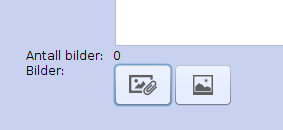
\includegraphics[trim=0cm 0.5cm 0cm 1.6cm,clip]{./img/produktdokumentasjon/bilder/1.png}
 \caption[Utsnitt fra boligbehandlingsvindu \# 1.]{Utsnitt fra boligbehandlingsvindu. Viser kontroller for opplastning og visning av bilder som er registrert for dette bildeobjektet.}
 \label{fig:bildebahndling}
\end{figure}

\begin{figure}[ht!]
 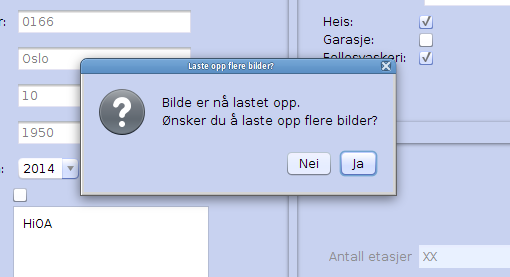
\includegraphics[width=\textwidth,height=\textheight,keepaspectratio,trim= 0cm 2cm 0cm 1cm,clip]{./img/produktdokumentasjon/bilder/2.png}
 \caption[Utsnitt fra boligbehandlingsvindu \# 2.]{Utsnitt fra boligbehandlingsvindu. Viser forespørsel til bruker (megler) dersom den ønsker å laste opp flere bilder for boligobjetet.}
 \label{fig:lasteoppbilder}
\end{figure}

\begin{figure}[ht!]
 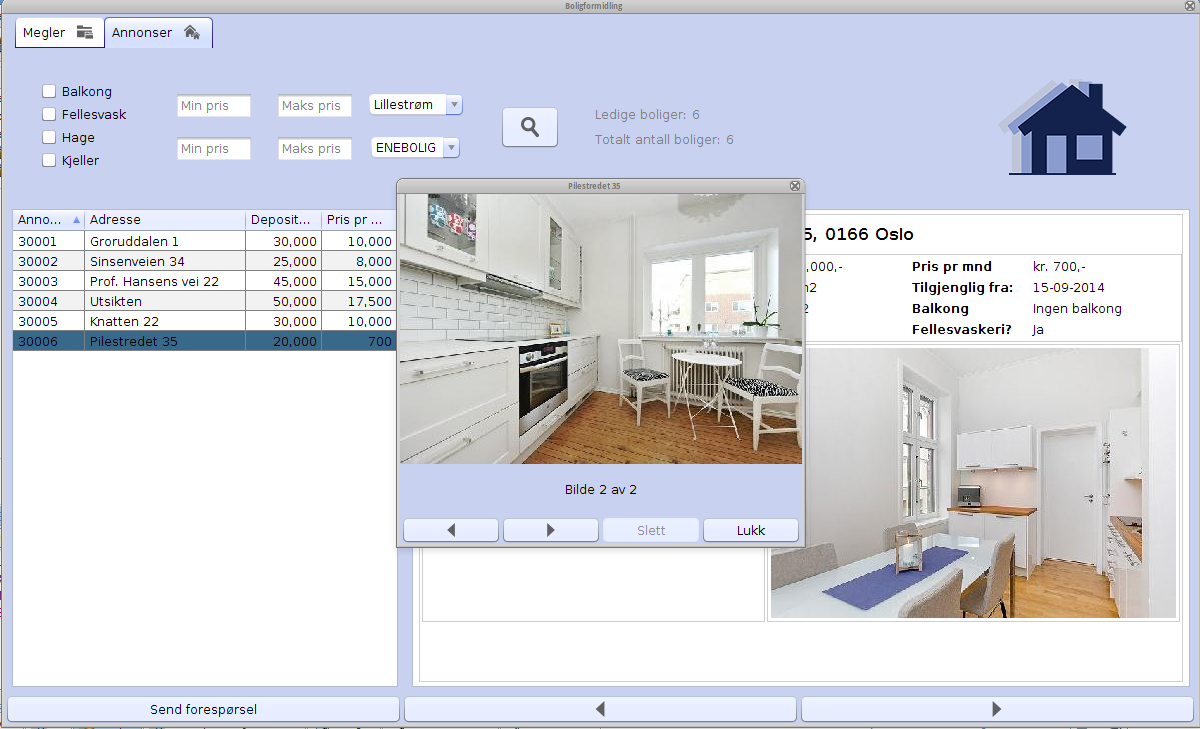
\includegraphics[width=\textwidth,height=\textheight,keepaspectratio]{./img/produktdokumentasjon/bilder/3.png}
 \caption[Bildevisning]{Bildevisning initialisert gjennom klikk i visningsarea for boligsøker.}
 \label{fig:bildevisning}
\end{figure}

\begin{figure}[ht!]
 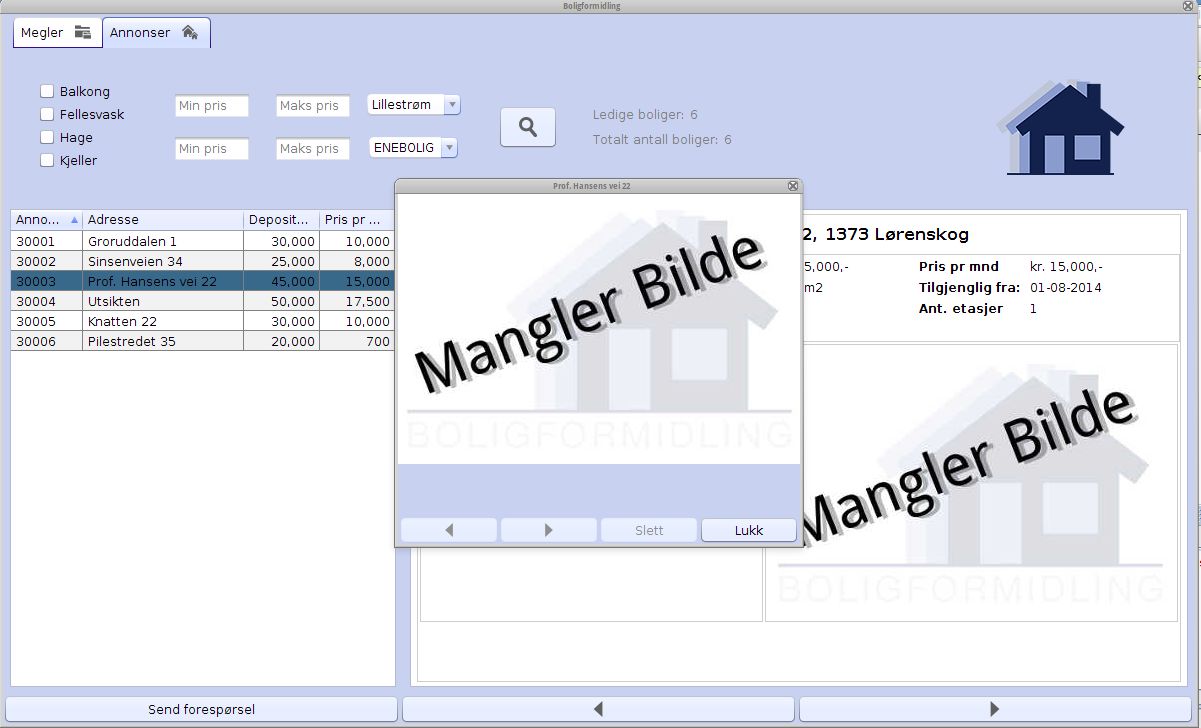
\includegraphics[width=\textwidth,height=\textheight,keepaspectratio]{./img/produktdokumentasjon/bilder/4.png}
 \caption[Standardbilde]{Eksepel på standardbilde som vises dersom brukeren ikke har lastet opp et bilde etter registrering av en ny bolig.}
 \label{fig:manglerbilde}
\end{figure}

\subsection{Sletting av bilder}
Sletting av bilder er foreløpig ikke implementert. Dersom et boligobjekt blir slettet må gallerimappen til boligen slettes manuellt. Det er tatt høyde for å implementere sletting og mulighet for dette er satt opp i brukergrensesnitet men foreløpig er deaktivert. 
\section{Konstanter og Enum}
Det er brukt konstater og flere enum typer i programmet, disse finner man i \texttt{lib} pakken. Konstanter er brukt i form av publike statiske variabler som er tilgjengelige tvers over alle pakker og klasser. Eksempel på dette er regex konstanter og konstanter som f.eks. brukes til å sette opp størrelse på GUI komponenter som vinduer eller teksfelt. 
Enum for å identifisere identifisere instanser av klasser eller klassevariabel isteden for å teste f.eks. på en streng som en identifikator. Eksempel på dette er data i en \texttt{comboboks}. Dersom vi fyller komboboksen med enumtyper kan vi direkte teste på hva som returneres til kontrollern fra gui isteden for å ta opp å bruke \texttt{equals()} metoden. 
Enum gir oss også mulighet til implementering av metoder direkte i enum klassen som kan foreta eventuelle beregniger på sine klassevariabler. 

\subsection{RegexTester.java} \label{subsec:regextest}
Klassen er satt sammen med hensikt å definere alle regext tester som foretas i programmet (oftest ved inhentning av data lagt inn fra bruker). 
Klassen består av publike regex konstanter som kan etter behov hentes opp av metoder der man kun etterspør en streng med et regex mønster, f.eks \texttt{CustomJTextField}.
Den andre delen av klassen består av boolean metoder som "<speiler"> alle regex streng konstanter og foretar et test på valgt regex kosntant og en mottatt tekststreng som parameter. 
I eksempel \ref{kode:regex1} presenteres en regex streng som brukes til å kontrollere en gateadress. Adressen må begynne med en stor bokstav, kan være opp til tre ord i lengden, deretter må avsluttes med et nummer opp til tre tall som kan blir etterfølgt av blankt steg og en bokstav (f.eks. trappeoppgang).

\begin{lstlisting}[caption=Regexstreng for gateadresse og husnummer.,label=kode:regex1]
	public static final String GATE_ADRESSE = "^[A-ZÆØÅ]{1}[a-zæøå]{1,20}[\\s]?[A-ZÆØÅ]?[a-zæøå]*[\\s]?[A-ZÆØÅ]?[a-zæøå]*[\\s][1-9]{1}[0-9]{0,2}?[\\s]?[A-ZÆØÅ]{0,1}$";
\end{lstlisting}

Eksempel \ref{kode:regex2} presenteres privat metoden som bruker Java
sin interne regex metode for å foreta test på mønsteret. Metoden blir kalt opp fra intern klasse som er spesiallaget for hver av regex konstantene (se neste eksempel).

\begin{lstlisting}[caption=Private regex test metode., label=kode:regex2]
	private static boolean patternMatchOK(String input, String regex) {
        try {
            erTestOK = input.matches(regex);
        } catch (PatternSyntaxException e) {
            System.out.println("Regex xception: input = " + input + " regex = " + regex);
        }
        return erTestOK;
  	}
\end{lstlisting}


I eksempel \ref{kode:regex3} presenteres som "<speiler"> hver enkelregex string konstant i klassen. Følgende metoder brukes i kontrollene som et andre kontroll trinn da et nytt objekt skal opprettes og legges til i registeret (første testet blir normalt foretatt i CustomJLabel med visuell \textit{feedback}). Ettersom metoden er \texttt{static} trenger den ikke å bli initialisert. 


\begin{lstlisting}[caption=Static regex metode til tilhørende regex møsnter streng., label=kode:regex3]
    public static boolean testGateadresse(String gateAdresse) {
        return patternMatchOK(gateAdresse, GATE_ADRESSE);
    }
\end{lstlisting}


\subsection{Konstanter.java} \label{subsec:konstanter}
Klassen består av flere publike konstanter lagret som static variabler som er tilgjengelige for alle klasser i programmet. I eksempel \ref{kode:konst1} presenteres noen av de konstantene som er satt opp i klassen som viser et kort utdrag for å presentere strukturen som brukes gjennom hele klassen.

\begin{lstlisting}[caption=Noen av static kosntanter som brukes i Konstanter klassen., label=kode:konst1]
    /**
     * Kollator rekkefølge som brukes til sortering.
     */
    public static final String KOLLATOR_REKKEFOLGE = "<\0<0<1<2<3<4<5<6<7<8<9"
            + "<A,a<B,b<C,c<D,d<E,e<F,f<G,g<H,h<I,i<J,j"
            + "<K,k<L,l<M,m<N,n<O,o<P,p<Q,q<R,r<S,s<T,t"
            + "<U,u<V,v<W,w<X,x<Y,y<Z,z<Æ,æ<Ø,ø<Å=AA,å=aa;AA,aa";

    /**
     * Felles serialiseringsnummer som brukes til unik nummer ved lagring av
     * programmets datastruktur.
     */
    public static final long SERNUM = 1234L;

    /**
     * En relativ path til alle eksterne filer som brukes i programmet som
     * serialisert data, bilder osv.
     */
    public static final String PROGRAMDATA = "programdata";

    /**
     * Serialisert fil som brukes til lagring og innlesning av all data i
     * programmet.
     */
    public static final String FILNANV = Konstanter.PROGRAMDATA + "/data.iso";
\end{lstlisting}

\subsection{GUI konstanter} \label{subsec:guikonst}
Følgende er konstanter som brukes for å sette opp en førdefiniert størrelse på alle komponenter i brukergrensesnittet. De består av to klasser:
\begin{description}

\item[\texttt{VinduStorrelse.java}]
En enum klasse som returnerer alle størrelse på vinduer som brukes i programmet. Den kan også brukes får å hente opp kun bredde eller høyde for et spesifikk vindu. Eksempel over klassens datafelt og  konstruktør presenteres i eksempel \ref{kode:guikonst1}. 

\item[\texttt{GuiSizes.java}]
En klasse med konstanter som brukes til nå sette opp interne \texttt{swing} komponenter som f.eks. bredde på \texttt{CustomJTextfield} eller \texttt{CustomJButton}.

\item[\texttt{Ikoner.java}]
Brukes til å hente opp referanser til alle ikoner som brukes tvers i hele programmet. Static konstanten blir satt opp som en \texttt{ImageIcon} variable som deretter kan brukes direkte for å sette opp et bilde i en \texttt{JPanel} eller liknende. Et kort eksempel over hvordan klassen er satt opp finnes i eksempel \ref{kode:guikonst2}.
\end{description}

\begin{lstlisting}[caption=Enum klasse for vindustørrelser, label=kode:guikonst1]
public enum VinduStorrelse {

    STOR (730, 1200),
    MIDDEL (600, 800), 
    LITEN (300,400),
    TOPPANEL (150,0),
    BUNNPANEL (30,0),
    VENSTREPANEL (0,400),
    SENTERPANEL (0,0);
    
    private final int WIDTH;
    private final int HEIGHT;

    private VinduStorrelse(int HEIGHT, int WIDTH) {
        this.WIDTH = WIDTH;
        this.HEIGHT = HEIGHT;
    }
	...
}
\end{lstlisting}


\begin{lstlisting}[caption=Utsnitt fra konstantklasse med static variabler for programikoner., label=kode:guikonst2]
public class Ikoner {

    private final static String ikonerSti = new BildeFilSti().getAbsoluteGalleryPath() + "/default/ico/";
	...
    //Tabs, 24px, 4px padding, farve 606060
    public final static ImageIcon ANNONSER = new ImageIcon(ikonerSti + "Houses-24.png");
    public final static ImageIcon MEGLER = new ImageIcon(ikonerSti + "Folder-Copy-24.png");
	...
    //Applikasjonsikoner, 128px, 0px padding, E8E8E8
    public final static ImageIcon APP_ICON = new ImageIcon(ikonerSti + "boligLogo.png");
    public final static ImageIcon NY_UTLEIER = new ImageIcon(ikonerSti + "ny_utleier.png");
    public final static ImageIcon NY_BOLIG = new ImageIcon(ikonerSti + "ny_bolig.png");
	...
}
\end{lstlisting}





\subsection{Enum}
I \texttt{lib} pakken er det satt opp flere klasser av enum type, en enum klasse ble forklart i avsnitt \ref{subsec:guikonst}. De resterende enum klassene som brukes i programmet er:
\begin{description}
\item[\texttt{Boligype.java}]
Definerer de forskjellige boligtypene som: \textit{Enebolig, Tomannsbolig, Rekkehus, Leilighet, Andre}. I programmet i dagens dato brukes det kun \textit{Enebolig} og \textit{Leilighet}. Enum klassen tar dog forbehold for viderutvikling av programmet gjennom å inkludere andre boligtyper.
\item[\texttt{Sivilstatus.java}]
Brukes for populering av kombobokser ved registrering av en ny boligsøker. Enum typen blir distribuert direkte mellom kombobks og kontroller.
\item[\texttt{Arbeidsforhold.java}]
Fungerer på sammen måte som \texttt{Sivilstatus.java} og brukes til sammen funksjoner i programmet med tar for seg boligsøkerens arbeidsforhold.
\item[\texttt{Objekttype.java}]
Brukes til å definere hvilken objekttype som sendes over i flere transaksjoner i programmet. Et eksempel på dette er renderering av tabell som blir satt etter hvilket objektytpe som er definiert i enum. 
Klassen spesifiserer objekttype på en øvre nivå, hvilket betyr at objektene blir spesifisert på superklasse nivå. Eksempelvis gjør denne enum typen ingen forskjell på objekttype \texttt{Utleier} eller \texttt{Leietaker} uten kan kun vise at objektet som sendes over er av type \texttt{Person}.
\item[\texttt{Objekttype2.java}]
Fungerer og brukes på samme måte som \texttt{Objekttype.java} med inneholder detaljert informasjon over hvilke objekter som kan passeres mellom transaksjonene. Her gjør vi altså forskjell mellom underliggende klasser som \texttt{Utleier} og \texttt{Leietaker}.

\end{description}
\section[Swing komponenter]{Tilpassede \texttt{Swing} komponenter} \label{sec:swing}
I programmet er det brukt flere spesialtilpassede komponenter arvet fra swing klassen der vi har spesifisert størrelse, brukerinteraksjon eller andre tilpasninger for å slippe å gjøre dette hver gang en slik komponent brukes. Komponentene er plassert i pakke \texttt{view} og \texttt{view.register}. I dette avsnittet beskrives spesielt tilpassede komponenter som har spesifikk betydning for programmet.

\subsection{\texttt{AbstractPanel.java}} \label{subsec:AbstractPanel}
Abstractpanel som arver \texttt{JPanel} er klassen som ligger til grunn til alle paneler som er i bruk i programmet. Klassen har to konstruktører og har som regel følgende oppgaver:
\begin{itemize}
\item Setter størrelse (dimensjon) på panelet.
\item Setter bakgrunnfarge på panelet fra en global static konstant. Dette gjør at farve på all brukergrensesnitt i programmet enkelt kan endres.
\item Sette en \texttt{titleBorder} rundt komponenten med tittel fra den innkomne parameter \texttt{tittel}. 
\end{itemize}
Dimensjonen settes ved å kalle opp metoden \texttt{setPrefferedSize(Dim dim)} som brukes ettersom slik tilnærming gjør at størrelse på panelet blir "<respektert"> av valgt layout manager (dette gjelder ikke alltid dersom \texttt{setSize()} brukes).




\subsection{\texttt{MainPanel.java}}
MainPanel er klassen som arver AbstractPanel og setter opp både megler og annonse-panelet, se eksempel \ref{kode:main_panel}. Arv fra superklassen består av at man kaller opp en tom konstruktør i superklassen som setter opp bakgrunnfarve. Deretter blir det satt opp en enkel \texttt{GridLayout} som består av én celle. Det vil si den dekker hele vinduet. Det legge til en \texttt{JTabbedPane} som legger til panel for annonse og megler. Annonsepanelet og meglerpanelet er igjen to klasser det kommes tilbake til i de neste avsnittene. Klassen \texttt{MainPanel} blir initialisert fra \texttt{StartGUI.java} ved oppstart av programmet, der de ferdigopprettede \texttt{ArkfaneMegler.java} og \texttt{ArkfaneAnnonse.java} sendes med som parametere for å kunne legges inn i \texttt{JTabbedPane}.


\begin{lstlisting}[caption=Kontruktør i \texttt{MainPanel.java},label=kode:main_panel]
    public MainPanel(AbstraktArkfane megler, AbstraktArkfane annonse){
        setLayout( new GridLayout( 1, 1)) ;
        this.megler = (JPanel) megler;
        this.annonse = (JPanel) annonse;
        
        arkfaner = new JTabbedPane(JTabbedPane.TOP);
        
        //Legger til tab og kobler med panelet.
        
        arkfaner.addTab("Megler  ", Ikoner.MEGLER, this.megler);
        arkfaner.addTab("Annonser  ", Ikoner.ANNONSER, this.annonse);
        
        arkfaner.setSelectedIndex(1);
        arkfaner.setToolTipTextAt(0, "Administrering av boliger, søknader mm.");
        arkfaner.setToolTipTextAt(1, "Finn tilgjengelige boliger, send inn søknader mm.");
        
        add(arkfaner);
    }
\end{lstlisting}



\subsection{\texttt{AbstraktArkfane.java}}
\texttt{AbstractArkfane.java} arver \texttt{AbstractPanel.java}. Klassene som arver \texttt{AbstracrArkfane.java} får et oppsett av paneler. Hvilket oppsett av paneler som blir opprettet er avhengig av hvilken parameter som blir sendt inn i konstruktøren, se eksempel \ref{kode:arkfane}. Hvilken type av arkfane som skal bli opprettet bestemmes a strengparameteren som blir sendt inn til konstruktøren. Klassen arves av to klasser: \texttt{ArkfaneMegler.java} og \texttt{ArkfaneAnnonse.java}, som utgjør de to arkfanene i programmet. 

\begin{lstlisting}[caption=Konstruktør til \texttt{AbstraktArkfane}.,label=kode:arkfane]
    public AbstraktArkfane(String valgtToppanel) {
        setLayout(new BorderLayout());
        setVisible(true);
        
        bunnpanel = new BunnPanel(VinduStorrelse.BUNNPANEL.getHEIGHT(), 
                VinduStorrelse.BUNNPANEL.getWIDTH());
        venstrepanel = new VenstrePanel("Liste",VinduStorrelse.VENSTREPANEL.getHEIGHT(), 
                VinduStorrelse.VENSTREPANEL.getWIDTH());
        senterpanel = new SenterPanel("Visning",VinduStorrelse.SENTERPANEL.getHEIGHT(), 
                VinduStorrelse.SENTERPANEL.getWIDTH());

        if (valgtToppanel.equals("megler")) {
            toppanel = new TopPanelMegler("Søk",VinduStorrelse.TOPPANEL.getHEIGHT(), 
                    VinduStorrelse.TOPPANEL.getWIDTH());
            add(toppanel, BorderLayout.NORTH);
        } else{
            toppanel = new TopPanelAnnonse("Søk",VinduStorrelse.TOPPANEL.getHEIGHT(), 
                    VinduStorrelse.TOPPANEL.getWIDTH());
            add(toppanel, BorderLayout.NORTH);
        }
        add(venstrepanel, BorderLayout.WEST);
        add(senterpanel, BorderLayout.CENTER);
        add(bunnpanel, BorderLayout.SOUTH);
    }
\end{lstlisting}



Som vi kan se i koden, AbstraktArkfane setter opp komponenter som inngår i de to visningsfanene fordelt på \texttt{Annonse} eller \texttt{Megler}. Klassen inneholder også en \texttt{LayoutManager} som setter opp alle disse komponentene med retninger: NORTH, WEST, CENTER og SOUTH. Resultatet av dette presenteres i figur \ref{fig:asbtarkfane} der de forskjellige panelene i klassen er satt opp. Klassen består også av et antall get-metoder som kan brukes til å returnere hele paneler til kontrollere i MVC-strukturen. Klassen blir arvet av følgende subklasser: (1) \texttt{ArkafaneAnnonse.java} og (2) \texttt{ArkfaneMegler.java}. Hver enkelt av disse subklassene kaller opp konstruktøren i superklassen \texttt{AbstraktArkfane} som initialiserer layouten og setter opp riktige paneler.




\begin{figure}[ht]
 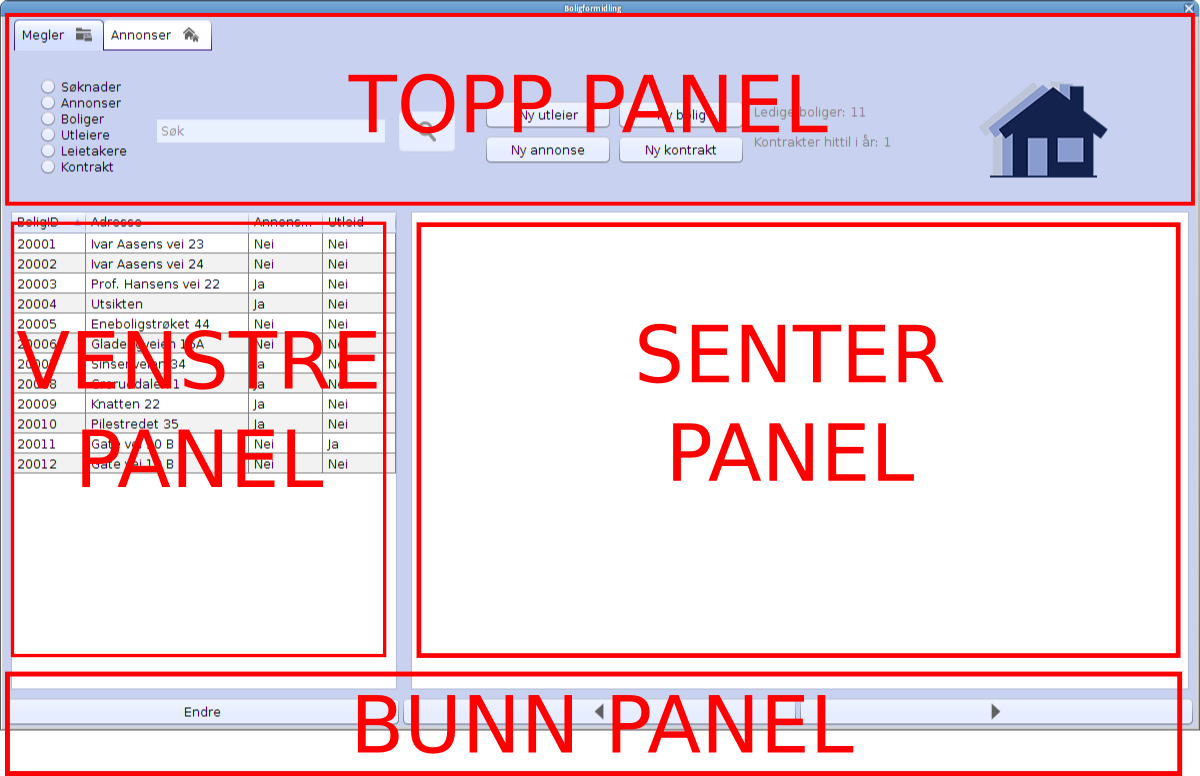
\includegraphics[width=\textwidth,height=\textheight,keepaspectratio]{./img/produktdokumentasjon/swing_componenter/AbstraktArkfane.png}
 \caption[Komponenter i AbstraktArkafane]{Fordeling mellom komponenter i AbstraktArkfane}
 \label{fig:asbtarkfane}
\end{figure}



\subsection{\texttt{TopPanelMegler.java}} \label{subsec:meglerpanel}
Toppanelet i meglervinduet (figur \ref{fig:megler_panel}) er kontrollert fra \texttt{ControllerToppPanelMegler.java}, komponentene i det toppanelet blir aktivert og deaktivert avhengig av hvilket register eller funksjon brukeren har valgt. Eksempel på dette er når brukeren første gang etter programstart går inn til panelet, da vil søkefeltet være deaktivert frem til riktig radioknapp velges for det register som man ønsker å søke i. Liknende funksjonalitet er lagt inn dersom man f.eks. ønsker å registrere en ny bolig. En bolig kan kun registreres på en "<person"> som i dette tilfelle kan være en eier eller en representant. For at man ikke skal ha mulighet til å registrere en bolig uten en eier er det allerede sperret på GUI slik at brukeren må markere en allerede registrert eier i utleierlisten og deretter klikke på "<\texttt{Ny bolig}">-knappen. Så lenge ingen person er markert i tabellen vil knappen forbli deaktivert. Tilsvarende den funksjonaliteten er det lagt til liknende begrensninger for opprettelse av en ny annonse, da det må markeres et boligobjekt i tabellen for å få lov å opprette en ny annonse. For å opprette en nytt kontrakt må det ha ankommet en forespørsel/søknad til megleren, som først markerer forespørselen for hvilken kontrakt skal opprettes. 

\begin{figure}[ht]
 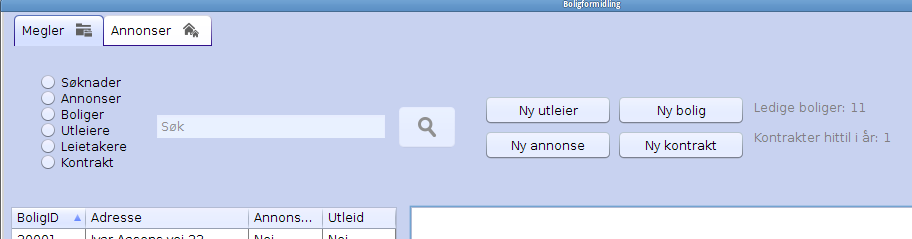
\includegraphics[width=\textwidth,height=\textheight,keepaspectratio]{./img/produktdokumentasjon/swing_componenter/megler_panel.png}
 \caption{GUI komponenter i meglerpanel}
 \label{fig:megler_panel}
\end{figure}




\subsection{\texttt{CustomSubPanel.java}}
Klassen arver den abstrakte klassen \texttt{AbstractPanel.java} (avsnitt \ref{subsec:AbstractPanel}). Den brukes til å sette opp indre paneler i alle registreringsvinduer som f.eks. registrering av nye boliger, utleier osv. Klassen er utstyrt med flere konstruktører som kan ta flere kombinasjoner av tittel, dimensjoner og layout manager. Slik valgfrihet gjør at panelet kan initialiseres på mange forskjellige måter og enkelt kan benyttes ut fra forskjellige behov som kan en har til brukergrensesnittet. Panelet inneholder også en metode for å ta imot en lytter (\texttt{ActionListener}) for en enkel og rask implementering sammen med en kontrollerklasse etter MVC-arkitektur.








\subsection{\texttt{CustomJTextField.java}}
\texttt{CustomJTextField} arver \texttt{AbstractPanel} og dermed inneholder samme konstruktør som det panelet, hvilken setter feltets dimensjoner. Slik løsning medfører også at hvert tekstfelt er plassert i en egen \texttt{JPanel}\footnote{arves av \texttt{AbstractPanel}}.
Tekstfeltet er spesialtilpasset slik at en den inneholder en indre label som kan for eksempel brukes til å sette en mal på hva brukeren skal skrive inn i tekstfeltet. Eksempelvis kan dette være forventet antall siffer i et telefon- eller personnummer, figur \ref{fig:custom1}. Feltet inneholder også to lyttere for \texttt{focusEvent} som initialiserer en regex etter et regex-mønster som settes via feltets konstruktør. Regex-mønster hentes via static konstanter som passer det uttrykk som feltet skal brukes til (se avsnitt \ref{subsec:regextest}, side \pageref{subsec:regextest}). Etter at markøren flyttes ut fra feltet, og regex-testen feiler, blir feltet markert med rød farve som det vises i figur \ref{fig:custom2}.
Panelet overrider også de metoder som man ønsker at skal være tilgjengelige fra superklassen \texttt{JTextField} som er \texttt{getText()}, \texttt{setText()} og \texttt{setEnabled()}.

\begin{figure}[ht!]
\centering
\begin{subfigure}[b]{1\textwidth}
\centering


\includegraphics[scale=0.7]{./img/produktdokumentasjon/swing_componenter/1.png}
\caption{Inaktiv, indre label}
\label{fig:custom1}
\end{subfigure}
\quad

\begin{subfigure}[b]{1\textwidth}
\centering

\includegraphics[scale=0.7]{./img/produktdokumentasjon/swing_componenter/2.png}
\caption{Regex-kontroll feilet}
\label{fig:custom2}
\end{subfigure}
\quad

\caption{Forsjellige tilstand av CustomJPanel}\label{fig:customjpane}
\end{figure}



\subsection{\texttt{CustomJButton.java}}
Klassen arver \texttt{JButton} og består av totalt fem forskjellige konstruktører (se eksempel \ref{kode:customButton} som brukes til å sette opp en spesifikk knapp. Konstruktørene er spesifisert på en måte slik at det kan settes opp knapper med forskjellige størrelser, titler, ikoner eller også kombinasjoner av alle disse mulighetene. 

\begin{lstlisting}[caption=De forskjellige konstruktørene i \texttt{CustomJButton}. ,label=kode:customButton]
public class CustomJButton extends JButton {

    private String navn;
    private Icon ikone;

    public CustomJButton(String navn) {
        this.navn = navn;
        setText(this.navn);
    }

    public CustomJButton(String navn, int bredde, int hoyde) {
        this.navn = navn;
        setText(this.navn);
        setPreferredSize(new Dimension(bredde, hoyde));
    }

    public CustomJButton(String navn, Icon ikone) {
        this.navn = navn;
        this.ikone = ikone;
        setText(this.navn);
        setIcon(this.ikone);
    }

    public CustomJButton(Icon ikone) {
        this.ikone = ikone;
        setIcon(this.ikone);
    }

    public CustomJButton(Icon ikone, int bredde, int hoyde) {
        this.ikone = ikone;
        setIcon(this.ikone);
        setPreferredSize(new Dimension(bredde, hoyde));
    }
}
\end{lstlisting}





\subsection{\texttt{ComboDatoVelger.java}}
Datovelger implementerer \texttt{CustomSubPanel} men hjelp av en egen layout manager. Klassen brukes med for å implementere en datovelger som skal gjøre det mulig for å velge riktig dato uten å bruke regex hvilket i sin tur skal oppleves enklere for brukeren. Komponentene består av tre \texttt{JComboBox} som brukes for valg av år, måned og deretter dag. Velgeren er utstyrt med en egen lytter som setter riktig antall dager i den siste listen etter at brukeren har valgt år og måned (se figur \ref{fig:combo_datovelger}).
Klassen kan returnere valgt data som \texttt{int} fordelt per år, måned og dag eller et \texttt{Calender}-objekt dersom så ønskes. Dato kan også blir satt gjennom å kalle opp metoden \texttt{setDato(int ar, int mnd, int dag)} som  er en funksjon som brukes ved f.eks editering av de registrerte boligene. 


\begin{figure}[ht]
\center
 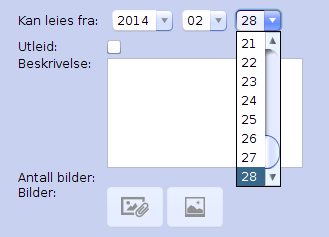
\includegraphics[scale=0.5]{./img/produktdokumentasjon/swing_componenter/combo_datovelger.png}
 \caption[\texttt{ComboDatoVelger.java}]{\texttt{ComboDatoVelger.java} tilpasning av antall dager.}
 \label{fig:combo_datovelger}
\end{figure}


%\section{Brukerinteraksjon}
\section{Visuelle detaljer}


\subsection{Ikoner}
Figur \ref{fig:appikoner} presenterer alle applikasjonsikonene som brukes til vinduene i programmet. Alle ikoner til subvinduer er satt sammen av våre egne ikoner og "<open source">-ikoner (se \ref{subssec:utvmiljo}, side \pageref{subssec:utvmiljo}). Hensikten med slike komposittikoner er at de skal gi en mer visuell tilbakemelding til brukeren som viser hvilken aktuelle funksjon som som brukes i programmet. 

\begin{figure}[ht!]
\centering
\begin{subfigure}[b]{0.2\textwidth}
\centering

\includegraphics[scale=0.4]{./img/produktdokumentasjon/visuelle_detaljer/boligLogo.png}
\caption{Programikonet}
\end{subfigure}
\quad
\begin{subfigure}[b]{0.2\textwidth}
\centering

\includegraphics[scale=0.4]{./img/produktdokumentasjon/visuelle_detaljer/ny_bolig.png}
\caption{Ny bolig}
\end{subfigure}
\quad
\begin{subfigure}[b]{0.2\textwidth}
\centering

\includegraphics[scale=0.4]{./img/produktdokumentasjon/visuelle_detaljer/ny_utleier.png}
\caption{Ny utleier}
\end{subfigure}
\quad
\begin{subfigure}[b]{0.2\textwidth}
\centering

\includegraphics[scale=0.4]{./img/produktdokumentasjon/visuelle_detaljer/edit.png}
\caption{Endre}
\end{subfigure}
\quad
\begin{subfigure}[b]{0.2\textwidth}
\centering

\includegraphics[scale=0.4]{./img/produktdokumentasjon/visuelle_detaljer/foresporsel.png}
\caption{Forespørsel}
\end{subfigure}
\quad
\begin{subfigure}[b]{0.2\textwidth}
\centering

\includegraphics[scale=0.4]{./img/produktdokumentasjon/visuelle_detaljer/bildevindu.png}
\caption{Bilder}
\end{subfigure}
\quad
\begin{subfigure}[b]{0.2\textwidth}
\centering

\includegraphics[scale=0.4]{./img/produktdokumentasjon/visuelle_detaljer/passord.png}
\caption{Pålogging}
\end{subfigure}
\quad
\caption{Applikasjons og vinduikoner}\label{fig:appikoner}
\end{figure}


\subsection{Presentasjon}
Figur \ref{fig:presentasjon} viser eksempel på hvordan objektene vises i \texttt{JEditorPane} gjennom \texttt{html}-visning. Datafelt for objektet "pareses" i klassen \texttt{ControllerOutput.java} i en metodene som er tilpasset til visning av spesifikt objekt, f.eks boligobjektene vises gjennom \linebreak \texttt{visBoligObjektHTMLOutput(Object valgtObjekt, JEditorPane output, AbstraktArkfane vindu, HashSet<Bolig> boligliste)}. Det er noen begrensninger i forhold til html visningen da \texttt{JEditorPane} er kun kapabel til visning av Html versjon 3.2 og CSS 1.0 fra 1997 (dette diskuteres utførlig i avsnitt \ref{subsec:contout}, side \pageref{subsec:contout}). 

\begin{figure}[ht!]
 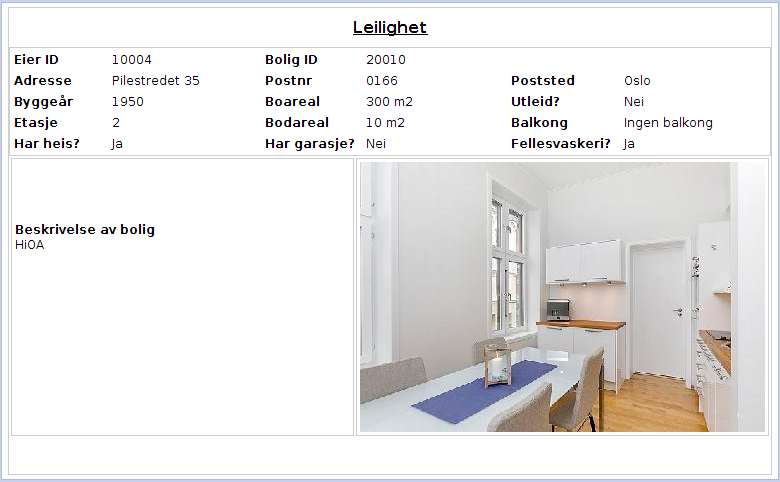
\includegraphics[width=\textwidth,height=\textheight,keepaspectratio]{./img/produktdokumentasjon/visuelle_detaljer/presentasjon.png}
 \caption{HTML presentasjon av et boligobjekt.}
 \label{fig:presentasjon}
\end{figure}


\subsection{Tabell}
I figur \ref{fig:tabell} presenteres utseende på formatert tabellobjekt, der annenhver rad har en annen bakgrunnsfarge og får en tredje bakgrunnsfarge ved markering. Forskjellige farger brukes i tillegg til horisontale linjer med hensikt å oppnå en bedre avskilt linje mellom presentasjonen av tabellkomponenter. Alle tabeller i programmet har også inkludert en meny som hører til de forskjellige objektene utfra hvilke funksjoner i programmet som kan brukes på et vist objekt. For eksempel i en tabell over boligobjekter. Boligobjekter kan man endres, slettes eller endre publiseringsstatus. Dersom brukeren "<skriver ut"> innhold i utleierregisteret vil det bli presentert alternativer som er spesifikke for objekter som instansierer superklassen person (ny endre, slett) men i tillegg funksjoner som er spesifikke for klassen utleier (som presentert i den refererte figuren). I eksemplet har vi mulighet å markere en person direkte og gå til registreringsdialog for bolig som da registreres på den personen. Vi kan også editere boliger som tilhører denne eieren eller også slette dem. Sammen funksjonalitet er også da tilgjengelig via den vanlige og synlige gui-komponenter som knapper eller også gjennom å dobbelklikker i tabellen.

\begin{figure}[ht!]
\center
 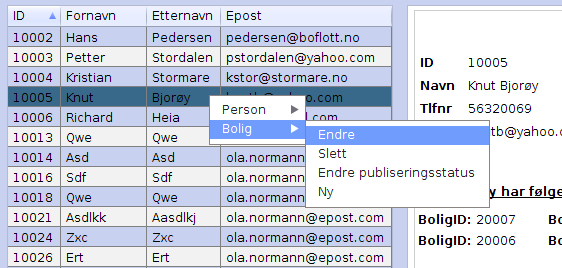
\includegraphics[scale=0.7]{./img/produktdokumentasjon/visuelle_detaljer/tabell.png}
 \caption{Visning og markering i tabell}
 \label{fig:tabell}
\end{figure}

\subsection{Grafisk tema}
Med tanke på å få bedre portabilitet mellom forskjellige operativsystem er standard Java "<LookAndFeel"> endret fra \texttt{Metal} til det nyeste swing tema \texttt{Nimbus}. Den primære årsaken til dette er at det ble observert noen forskjeller på størrelse og layout av gui-komponenter mellom operativsystemene som programmet var testet på. Eksempelvis, dersom programmet testes i Linux miljø finnes det ingen "<native"> grafisk miljø i form av komponenter som knapper, men på Mac OS og MS Windows der Java er kapabel å renderere standard knapper for systemet ble det noen forskjeller mellom slike komponenter. Bruk av nimbus som primær tema for gui komponenter gir sikkerhet at alle kompoenentene kommer til å bli renderert gjennom JVM hvilket gir en god portabilitet mellom operativsystemene (også beskrevet i avsnitt \ref{subsec:portabilitet} "<protabilitet">, side \pageref{subsec:portabilitet}).

\begin{figure}[ht!]
\centering
\begin{subfigure}[b]{0.3\textwidth}
\centering
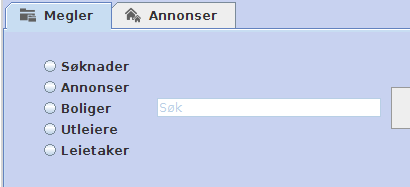
\includegraphics[trim=0cm 0cm 7cm 0cm, clip,scale=0.5]{./img/produktdokumentasjon/visuelle_detaljer/metal.png}
\caption{Stadard tema "<metal">}
\end{subfigure}
\begin{subfigure}[b]{0.3\textwidth}
\centering
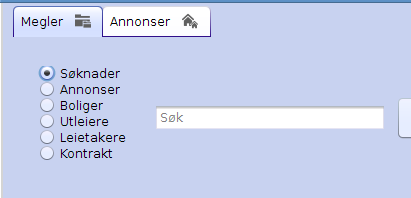
\includegraphics[trim=0cm 0cm 7cm 0.2cm, clip,scale=0.5]{./img/produktdokumentasjon/visuelle_detaljer/nimbus.png}
\caption{Nimbus}
\end{subfigure}
\caption{Applikasjons og vinduikoner}\label{fig:tema}
\end{figure}

%\input{./tex/produktdokumentasjon/sdf}




%Her kommer eksmpler som vi kan bruke nå man skal lage latex i rapporten
%\chapter{Kort bruksanvisning i \LaTeX{}}

Stortingets Tibetkomité består av enkeltrepresentanter med et spesielt sterkt 
engasjement for Tibet. Etter stortingsvalget høsten 2013 tok Venstres Ketil 
Kjenseth på seg en koordinerende rolle, og sendte i januar ut en mail til alle 
stortingsrepresentanter om hvem som kunne tenke seg å bidra.
Til tross for at Høyre åpner sitt landsmøte på Gardermoen fredag formiddag har 
fem stortingsrepresentanter fra regjeringspartiet funnet plass i programmet til 
å møte tibetaneren: Michael Tetzschner, Heidi Nordby Lunde, Erik Skutle, Anders 
B. Werp og Peter Chr. Frølich. Også Unge Høyre-leder Paul Joakim Sandøy er med 
og tar imot Dalai Lama.

\section{Kode}
Her kommer litt javakode for å teste ut hvorda det kommer til å se ut.

\begin{lstlisting}[caption=Koden teller til 1000, label=brakode]
class KnappeLytter implements ActionListener {

        @Override
        public void actionPerformed(ActionEvent e) {
            if (e.getSource().equals(vindu.getLagreButton())) {
                if(erNyregistrering){
                    registrerNyLeietaker();
                }
            } else if (e.getSource().equals(vindu.getAvbrytButton())) {
                vindu.dispose();
            }
        }

    }
\end{lstlisting}


\section{Kode fra fil}
Slik kan man legge inn kode direkte fra en java fil

\lstinputlisting[caption=Koden her gir NullPointerException, label=java:test1]{./kode/latex_bruksanvisning/1.java}



\section{Liste}
Her kommer eksepel på en liste\footnote{Her legger man til en fotnot hvis man ønsker å kommentere noe.}
\begin{itemize}
 \item Epple
 \item Pære
 \item Frosker
 \item Banan
\end{itemize}



\section{Figurer}
\subsection{Eksempel 2}
\begin{figure}[ht]
 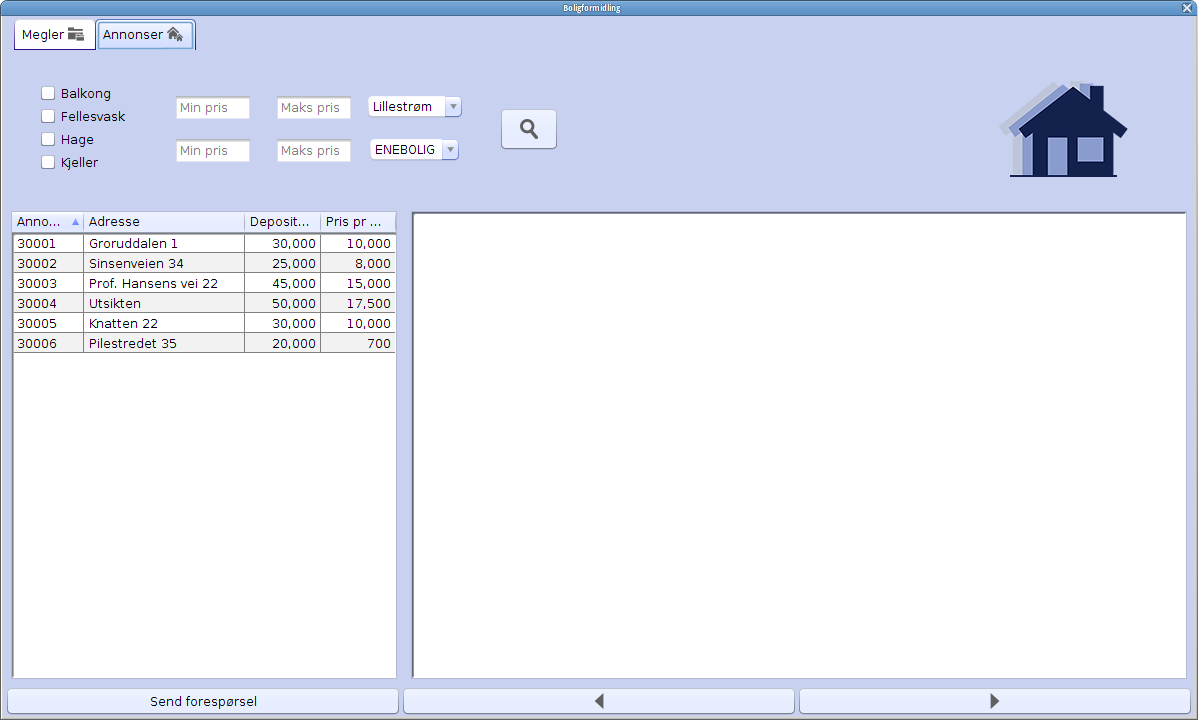
\includegraphics[width=\textwidth,height=\textheight,keepaspectratio]{./img/latex_bruksanvisning/1.png}
 \caption{Dette er et eksempelbilde. Bilde blir automatisk numerert og lagt til i registeret.}
 %Her kommer en kabel for kryssreferering i teksten til figuren
 \label{fig:hovedvindu}
\end{figure}

\section{Referering}
Man må referer til alle figurer og kodeeksempel, som regel skal det ikke finnes en figur eller kodeeksempel dersom man ikke refererer til det i teksten. For at man skal kunne referer til noe så må man ha \textit{label} tag. For eksempel kan man nå referer til bilde gjennom følgende \ref{fig:hovedvindu}. \\
Man kan også ta en referanse til code gjennom \ref{java:test1}



%Appendix for vedlegg og andre ting som ikke direkte passer inn i resten av rapporten
\appendix
\chapter{Funksjonalitet} \label{app:funksjonalitet}
Følgende tillegg beskriver i detalj noen av modulene som er tenkt at systemet skal inneholde ved første release.


\section{Tjenere (servers)}
Følgende modul skal brukes til å sette opp forskjellige servere på maskinene. Modulene kjøres som skript og setter ønsket funksjonalitet etter ønske. Under oppsettet av hver enkel tjener blir brukeren presentert med en “wizard” der man får lov til å velge ekstra funksjonalitet eller annen funksjon som eventuelt tilbys av programvaren (f.eks. virtuelle servere i Apache). Oppsett av tjenere er fullstendig modulbasert. Dette medfører at brukere kan etter ønske utvikle egne konfigurasjonsmoduler som kan publiseres og deles med andre studenter via systemets marketplace. 

\subsection{Apache webserver}
Modulen setter opp og konfigurerer apache webserver med tilhørende moduler. Brukeren blir presentert med en wizard som går igjennom følgende innstillinger og konfigurasjoner.
\begin{description}

\item[Mapper] Her kan brukeren sette opp hvilke mapper som skal være tilgjengelige på nett. Brukeren har mulighet til å sette opp flere mapper i sin hjemmemappe samt se en forhåndsvisning på hvordan nettadressen kommer til å se ut. Dersom brukeren har satt opp synkroniseringstjeneste (mer om dette under ...) blir det også mulig for brukeren å “peke” webserveradresse til en mappe i synkroniseringstjenesten. Dette vil da gjøre det mulig for brukeren til å oppdatere nettsiden fra en ekstern datamaskin som synkroniserer til samme tjeneste.

\item[Tilgang og sikkerhet] Her er det mulig å sette opp funksjoner som “directory browsing” og diverse sikkerhets innstillinger.

\item[Moduler] Aktivering av tilleggsmoduler som php og MySQL støtte. Valg av feks disse to vil laste ned og installere php samt MySQL database med standardinnstillinger.
\end{description}

\subsection{MySQL}
Modulen installerer, og setter opp bruker med samme brukernavn og passord som systemets  bruker. Etter ønske blir det også vist en “wizard” som viser brukeren hvordan man kan koble opp mot databasen og bruke denne. Etter ønske fra brukeren kan det også bli satt opp med software for enklere administrasjon av databasen, f.esk. MySQL Workbench. Det skal også gis mulighet til å konfigurere tabeller som brukes i fag som Databaser (se her etterkommende avsnitt om hobbyhuset). 

\subsection{SSH}
Alle *NIX baserte system kan kontrolleres via “secure shell”. Denne modulen vil sette opp en standard ssh-server på maskinen som gjør det mulig for brukeren å logge seg på fra en ssh klient.

\section{System}
Modulen system innholder moduler som brukes til systemkonfigurasjon og kontroll. Modulene her kan brukes til installere og konfigurere både programvare og medfølgende innstillinger på brukerens sin virtuelle maskin. 

\subsection{Programvare}
Her kan brukeren velge å installere moduler som er tilgjengelige via et sentralt repository for EasyDev. Brukeren kan velge å laste ned og installere nye moduler (programvare) eller slette en eksisterende modul.

\subsection{Oppstart}
Modulen gir brukeren mulighet til å velge hvilke prosesser som skal startes sammen med systemet. For eksempel dersom man ønsker at sammen med systemet skal startes Apache webserver og MySQL database. Dette velges utfra en liste med sjekkbokser som generes basert på de moduler som er installert på systemet.

\subsection{Brannmur}
Dersom man ønsker at systemet skal ha en brannmur blir det mulig for brukeren å sette opp slik funksjonalitet via brannmurmodulen. Brukeren kan med hjelp av denne modul implementere en brannmur som må ta høyde for de moduler som allerede kjører på systemet. Dette må gjøres for at brannuren ikke skal sperre eventuelle porter for inngående kommunikasjon som de ulike modulene bruker. Derfor skal det finnes en intern fil (eller database) som innholder all nødvendig informasjon om porter som skal holdes åpne dersom brannmuren blir konfigurert i etterkant. Oppsett av brannmuren skal foregå med hjelp av en “wizard” og konfigurasjons-gui der brukeren kan kontrollere de innstillinger som blir foreslått basert hvilken port som skal holdes åpen. Alle kommandoer som kjøres fra GUI skal også presenteres for brukeren i en nærliggende utskriftsvindu og i tillegg lagres i en loggfil. Hensikten med dette er at man skal ha mulighet til å studere den “manuelle” konfigurasjonen for egen læring.

\subsection{Brukere og grupper}
Her definerer man brukere og grupper og hvilke brukere som er med i hvilke grupper.
Denne modulen er tenkt brukt sammen med “Ressursene”, det vil si webområdene man har definert og databasene man har opprettet osv. 
Man kan her opprette brukere og legge dem i grupper. Gruppene kan da brukes som prosjektgrupper, og man får opp en liste med ressurser på maskinen der man kan huke av hvilke ressurser gruppen skal ha tilgang til. De brukerne som er medlemmer i gruppen vil da få redigeringsmulighet på de delte ressursene og mulighet til å laste opp og endre innhold.
Dette er en sentral funksjonalitet i forhold til å gi studentene en god plattform å jobbe med i prosjektoppgaver, og så langt vi har oversikt over er det en unik funksjonalitet som ikke tilbys i andre løsninger, hverken på HIOA eller i administrasjonsløsninger for Linux.

\subsection{Synkronisering}
Modulen skal gi mulighet for brukeren til å sette opp synkronisering til de mest vanlige skytjenestene som Dropbox, SkyDrive, Google Drive men også eventuelt hjelpe til å sette opp MyCloud dersom noen ønsker å benytte seg av en egen synkroniseringsløsning. 
Det skal være mulig å dele mapper innad i en gruppe. Tanken er at brukere kan direkte skrive inn gruppemedlemmenes studentnummer for å sende forespørsel til en synkronisert mappe. Denne funksjonen er mest sannsynlig kun mulig dersom man kjører en synkroniseringssky internt på skolens sine servere. 

\subsection{Systemoversikt}
Her skal det bli presentert forskjellige typer av systeminformasjon, som informasjon om aktuell OS kjerne, antall brukere, installerte moduler og tilgjengelig lagringsplass på samtlige partisjoner. 

\subsection{Logg}
En modul som tydelig viser all loggføring som foregår i “/var/log”. Det skal være enkelt for brukeren å identifisere hvilket program loggen kommer fra. Et eksempel er loggen fra Apache som er plassert i “/var/log/httpd.log”. Dette er selvsagt ingen brukervennlig måte å identifisere en loggfil. Brukeren skal ha mulighet til å velge at man ønsker å se loggfilen for Apache server, og man får så opp filens innhold og hvor filen er lagret på systemet. Det skal også være mulig å lese gamle loggfiler som har blitt komprimert av loggrotasjonsystemet. Det vil også være mulighet for å søke i loggfilene.

\subsection{Belastning}
Skal være en form av “widgets” og/eller statistikk som presenteres for brukeren om systemets “helse” og tilstand. Her skal det være mulig å lese av CPU belastnintg, tilgjengelig hukommelse, aktuelle operasjoner på platelager og prosessenes belastning. Man skal også få opp nettverksinformasjon og belastningen på de forskjellige enhetene.



\section{Ressurser}
Modulen består av forskjellige ressurser som kan være til god nytte i forskjellige fag. Det kan være alt fra gode linker til nettsider, til forskjellige verktøy som validering av kode. Innholdet her blir mest sannsynlig manuelt lagt til av studentene, avhengig av hvilket fag som er interessant for dem. Målet er også at modulene eventuelt kan utvikles av studentene selv slik at disse blir godt tilpasset til de fag som gis ved skolen. Det skal være mulig å rangere alle modulene etter for eksempel antall stemmer eller popularitet (antall nedlastninger).

\subsection{Validering}
I de fleste fag som har med webutvikling å gjøre er det krav at man skal validere oppgavene  man har laget slik at løsningen følger alle nødvendige standarder. Det er tenkt at under ressurskategorien skal det finnes tilgjengelig en modul som tillater å velge godkjente filtyper og kjøre online validering på disse. Dette vil da gjøre det enklere å raskt validere filene uten å  gjøre dem tilgjengelig/publisere på en webbserver eller laste dem opp til en tredjeparts side for validering.

\subsection{Nettressurser}
Mulighet for en rask tilgang til gode kunskaps resurser på nettett sortert etter fag. Dette kan for ekesempel være W3Shools, Udemy, Cave of Programming med mer.

\subsection{Regex-generator}
Det finner mange regex-generatorer tilgjengelige på nettet. Problemet med disse er at selve syntaksen for hvordan regexen skal valideres på de forskjellige sidene varierer. Med andre ord det tar tid å lære seg den enktlte regex validator som finnes på nettet, og som ofte krever disse at brukeren kan noe standard regex syntaks fra før. Det som skal tilbys via vårt system er at brukeren skal få mulighet til å bygge sin egen regex ut fra et enkelt grafisk grensesnitt som er en form av “logiske gater” eller “Venn” diagram der man skal angi hvilke typer av ASCII eller uttrykk som skal inkluderes eller ekskluderes for den aktuelle regex-streng. Ut over dette skal det også være mulig for brukeren å skrive inn sin egen regex og direkte teste denne den på ønskede strenger for å se om den fungerer. Eventuelt kan det implementeres en link til ressurser som viser hvordan regex kan implementeres i forskjellige språk og teknologier. Alt fra tolkningsrpåk som PHP, JavaScript til kompileringsspråk og de mest vanlige grafiske bibliotek som Swing, JavaFX, GTK+ eller Qt.

\subsection{SQL scripts}
Her kan det plasseres SQL-script som for eksempel “hobbyhuset” som kan brukes i faget Databaser. Andre script som backup av databaser, samt andre administrative script vil også finnes her.

\subsection{Versjonshåndtering}
Det er normalt ganske vanskelig å komme igang med et versjonskontrollsystem. En modul som ikke bare setter opp en av de mest populære versjonhånderingssystemene (f.eks. GIT) men også viser de mest vanlige prinsippene som er nødvendig for å starte med å jobbe i team der man bruker versjonshåndtering. Det kan være elementer som oppsett, staging, commits, branching, merging, diff samt push og pull til fjernservere. 



\section{Meldinger}
En integrasjon av studentepost direkte til systemet. Det skal tilsvare mer eller mindre samme funksjonalitet som i en webmail. 



\section{Verktøy}
Modulen skal bestå av praktiske verktøy som kan være til god hjelp dersom man trenger å gjøre endringer i konfigurasjon direkte på den virtuelle maskinen. Foreløpig tenker vi på de to verktøy som er til grunn og bunn viktigst for alle brukere: teksteditor og terminal.

\subsection{Editorer}
Integrert teksteditor som kan brukes til de fleste utviklingsspråk, med syntakshighlighting og syntakskontroll. En slik editor mest aktuell for språk som brukes i webutvikling ettersom det blir mulig å utvikle direkte på webserveren uten å koble til/montere mappen eller laste opp filene kontinuerlig til serveren. Editoren skal også gi mulighet til å kompilere kode. Dersom man bruker skriptspråk som html eller css skal det være mulig å validere syntaksen direkte fra editoren. Eventuelt skal det også implementeres støtte for versjonshåndtering. Eksempel på språk og script som skal støttes: Java, JavaScript, PHP, Html, SQL, CSS, C, bash.

\subsection{Terminal}
For å gjøre det enkelt å administrere systemet for mer erfarne brukere skal det også tilbys en modul som representerer en terminalemulator. Foreløpig er det noe uklart hvordan en slik terminal skal implementeres i en nettleser ettersom det er ønskelig å gir umiddelbar tilbakemelding til bruker som utskrift av resultat fra de kommandoer som kjøres i terminalen. Målet er å gi like god bruksopplevelse som man får ved bruk av terminal direkte på maskinen. 

\subsection{Filbehandler}
En enklere variant av en filbehandler som tillater bruker til å behandle filer på systemet sitt. Programmet skal følge samme rettigheter som man har på systemet slik at vanlige brukerrettigheter får brukeren kun behandle filer i sin egen hjemmemappe. Dersom man ønsker “root”-tilgang må man logge seg på med “root”-passord, dette vil gi en tilbakemelding til brukeren i form av at f.esk. programmet skifter farge til rød (skal signalisere fare ettersom med “root” tilgang er det fullt mulig å ødelegge systemet). 


Med tanke på læring er det viktig at brukeren kan se terminalutskrift for alle kommandoer som blir foretatt for filbehandlingsoperasjoner. Med andre ord, programmet skal oversette det som brukeren ønsker å gjøre grafisk i programmet til “bash” kommandoer. Eksempel på dette er hvis man ønsker å skifte navn på filA.txt til filB.txt vil brukeren bli presentert samtidig som operasjonen utføres med en utskrift ved siden som viser selve syntaksen for operasjonen. I dette tilfellet : \texttt{bash\$ mv filA.txt filB.txt}. Dette vil gi veldig god forståelse og eksempler på bruk av terminal i unix/linux/mac-miljøer.
\addcontentsline{lof}{chapter}{Tillegsfigurer}
\chapter{Prototyper}
I dette avsnitt blir det nærmere presentert bilder av prototyper. Hensikten er at vi ønsker å presenter bildene i bedre kvalitet enn hva som tillates inne i rapporten. Derfor valgte vi å plassere disse i spesill appendiks.
\section{Low-fi prototype}

\section{Hi-fi prototype}
\begin{figure}[ht]
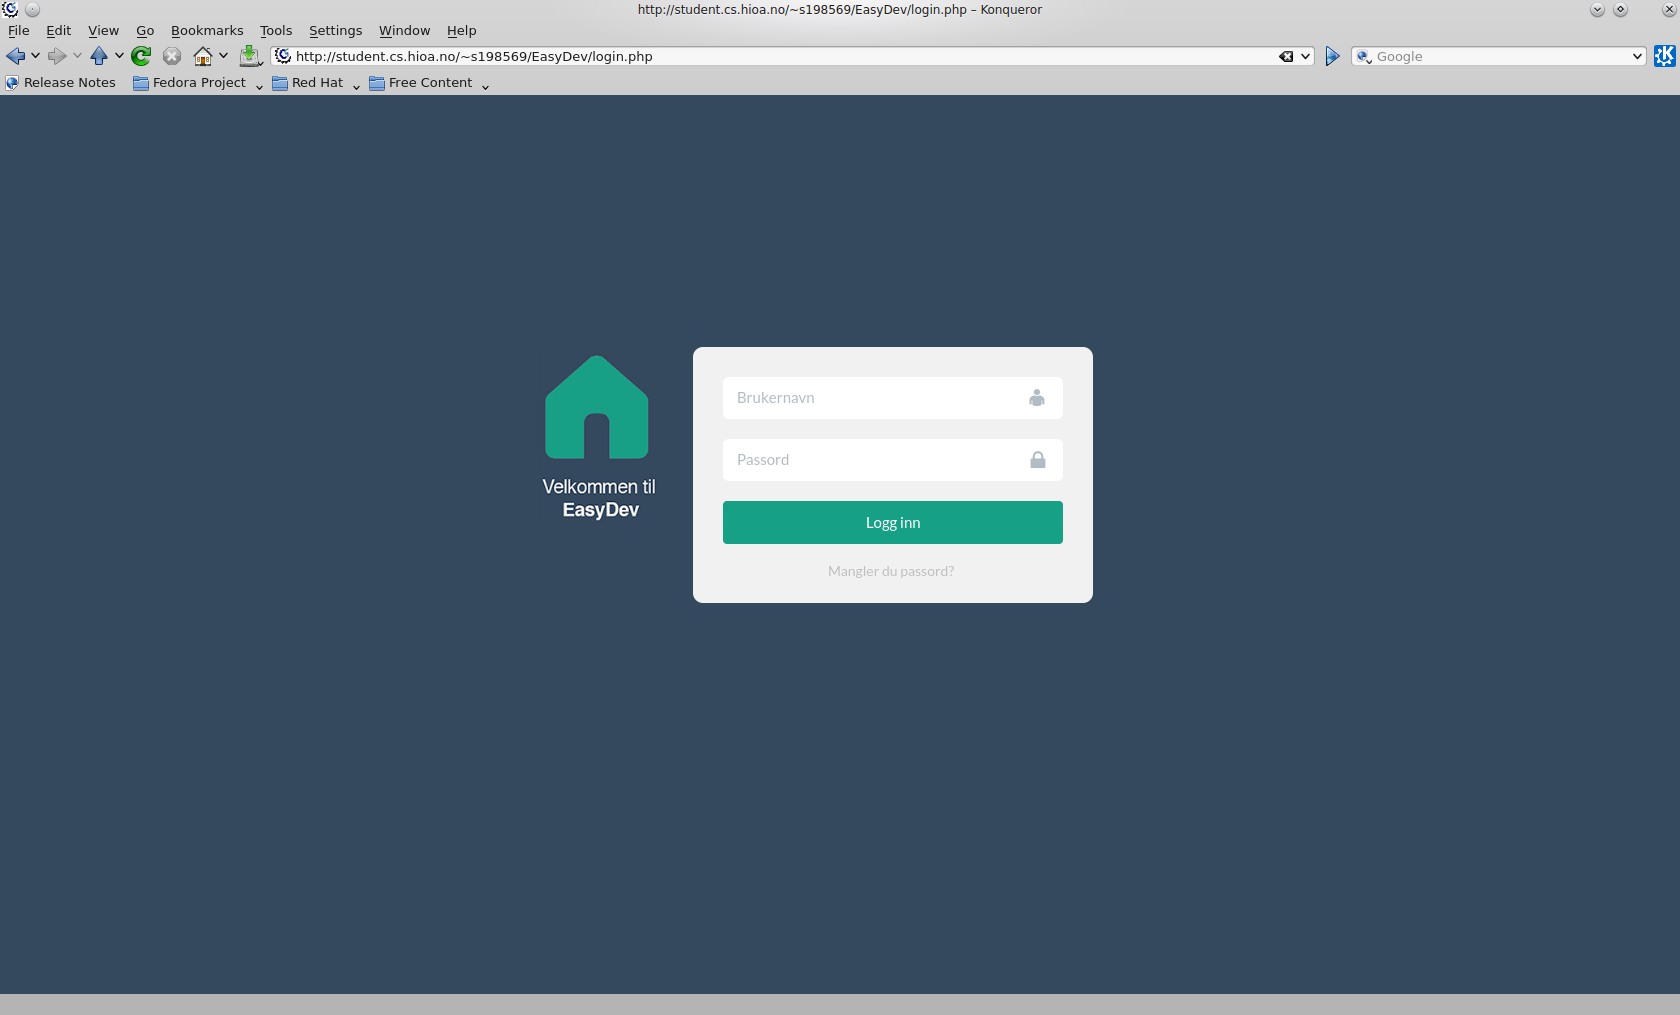
\includegraphics[width=\textwidth,height=\textheight,keepaspectratio]{./img/prosessdokumentasjon/hifi/login.png}
\caption[(Hi-fi) Påloggingsbilde]{Påloggingsbilde. I prtotypen er det mulig å logge seg på uten brukernavn eller passord. Etter dette påloggingsbilde blir brukeren forflyttet til fremside.}
\label{fig:loginhi}
\end{figure}

%KONFIGURASJON AV APACHE
\begin{figure}[ht]
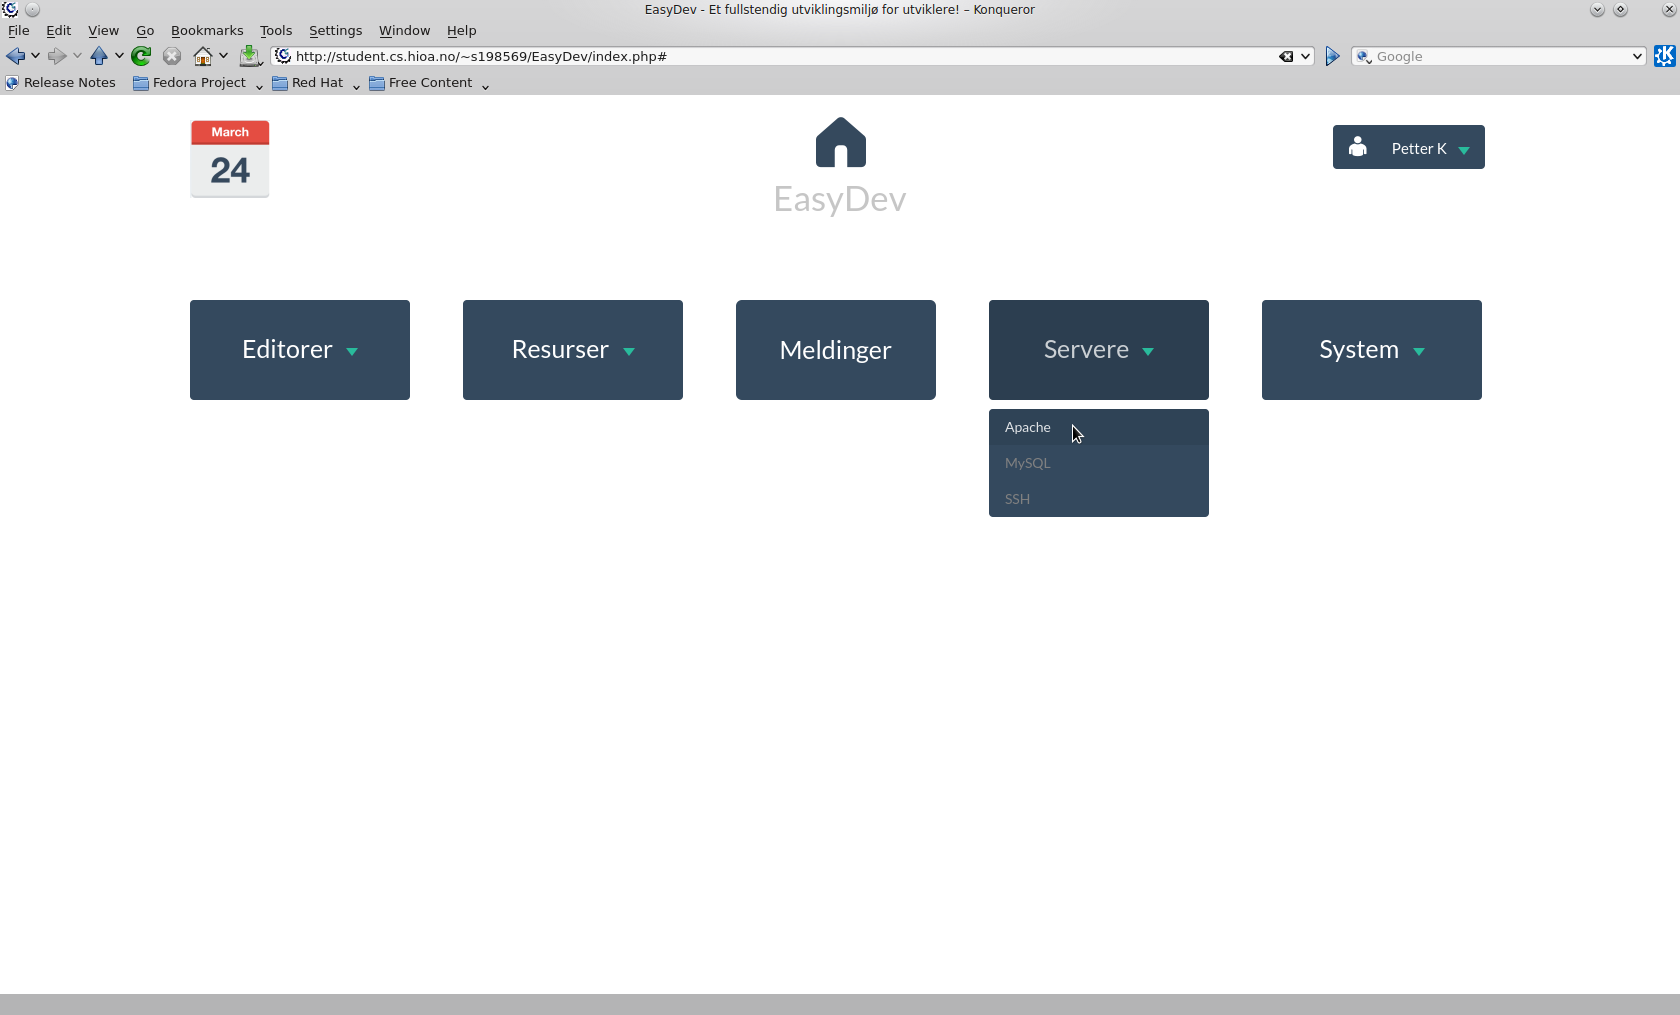
\includegraphics[width=\textwidth,height=\textheight,keepaspectratio]{./img/prosessdokumentasjon/hifi/a1.png}
\caption{(Hi-fi) Webserver: }
\label{fig:apachehi1}
\end{figure}

\begin{figure}[ht]
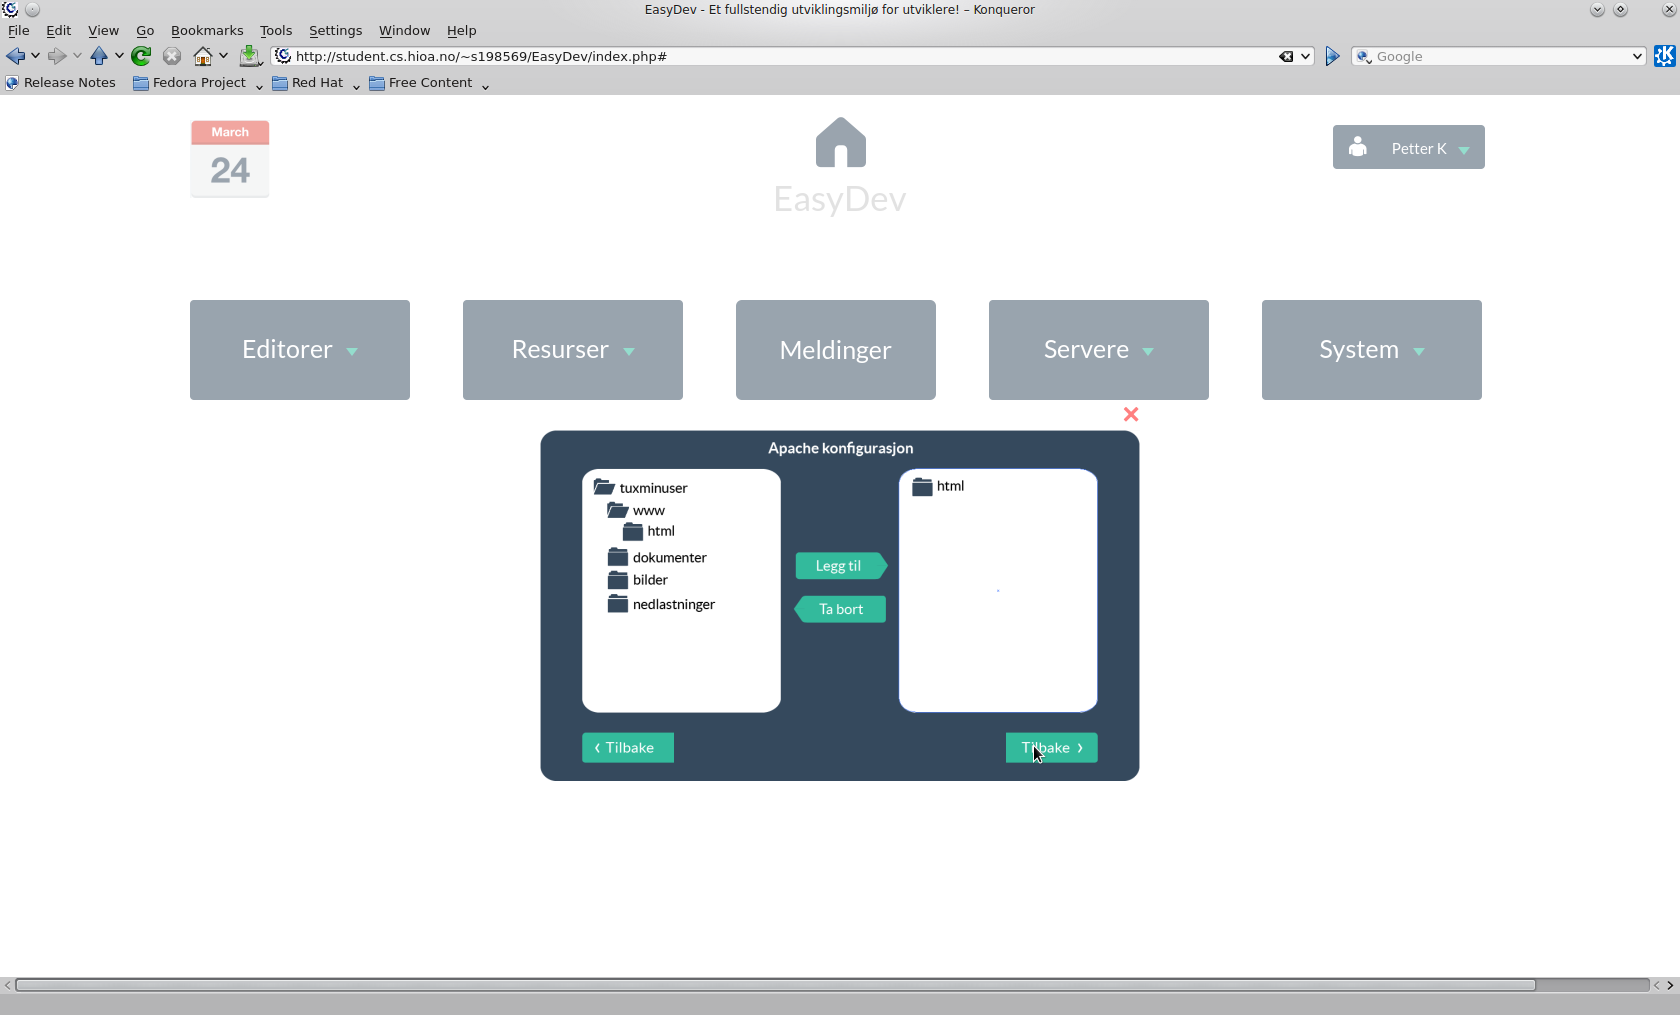
\includegraphics[width=\textwidth,height=\textheight,keepaspectratio]{./img/prosessdokumentasjon/hifi/a2.png}
\caption{(Hi-fi) Webserver: }
\label{fig:apachehi2}
\end{figure}

\begin{figure}[ht]
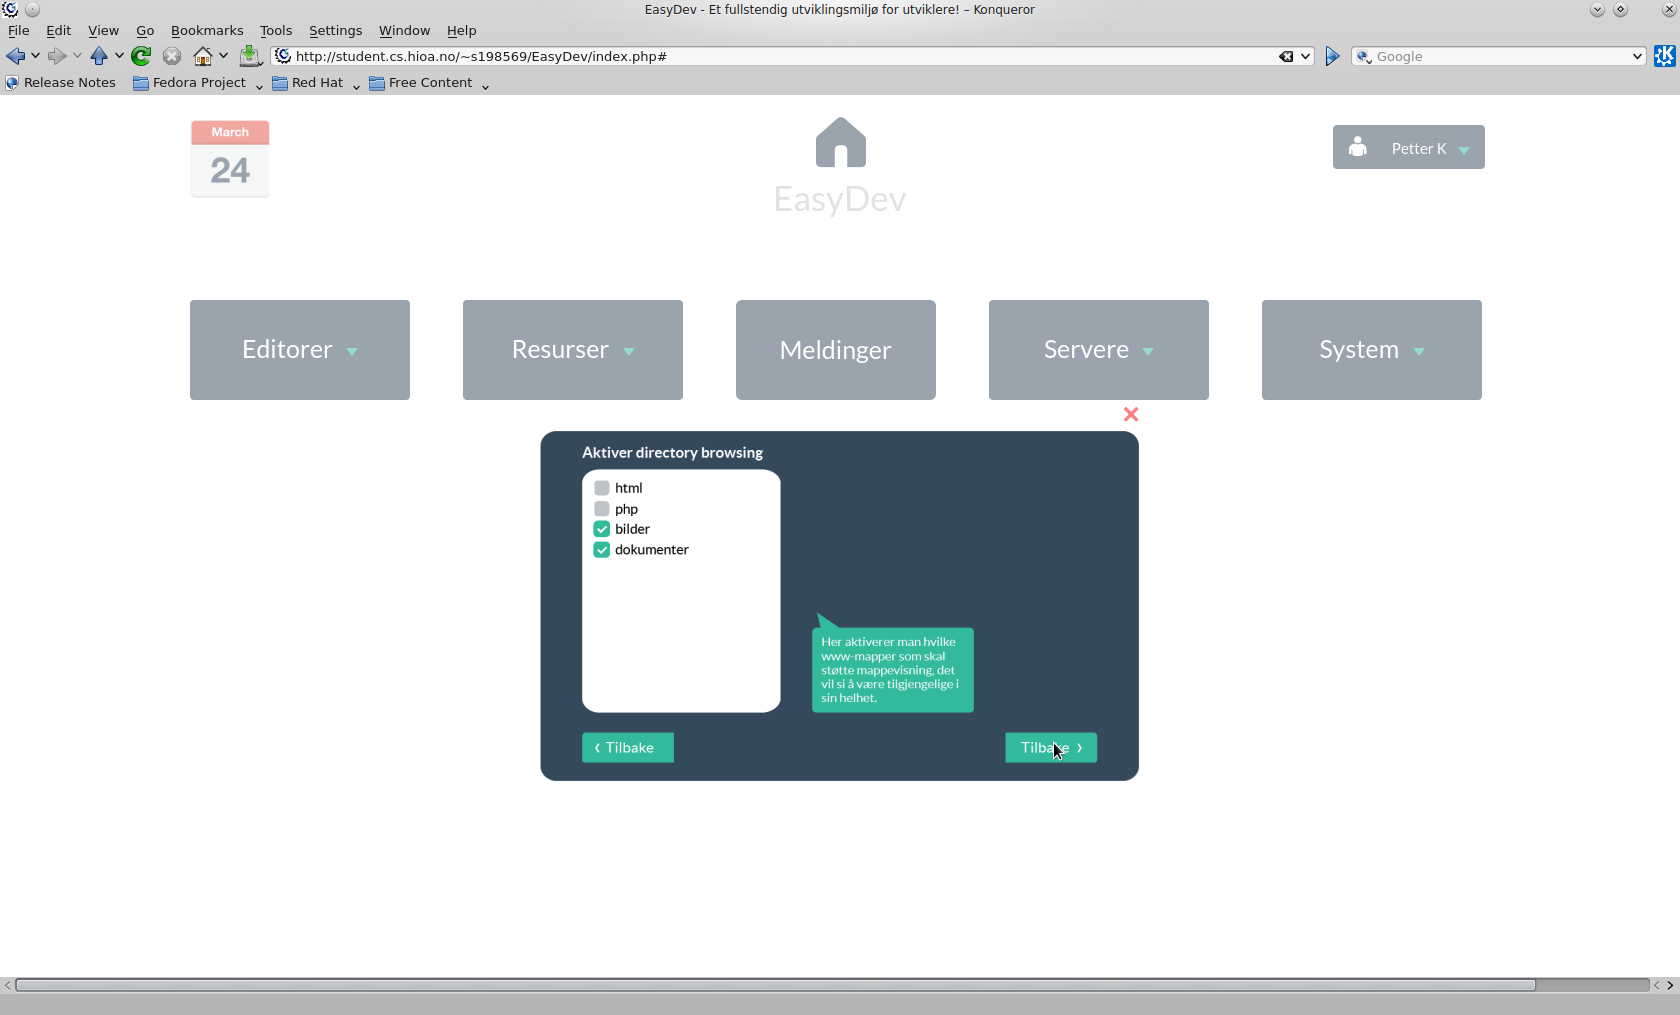
\includegraphics[width=\textwidth,height=\textheight,keepaspectratio]{./img/prosessdokumentasjon/hifi/a3.png}
\caption{(Hi-fi) Webserver: }
\label{fig:apachehi3}
\end{figure}

\begin{figure}[ht]
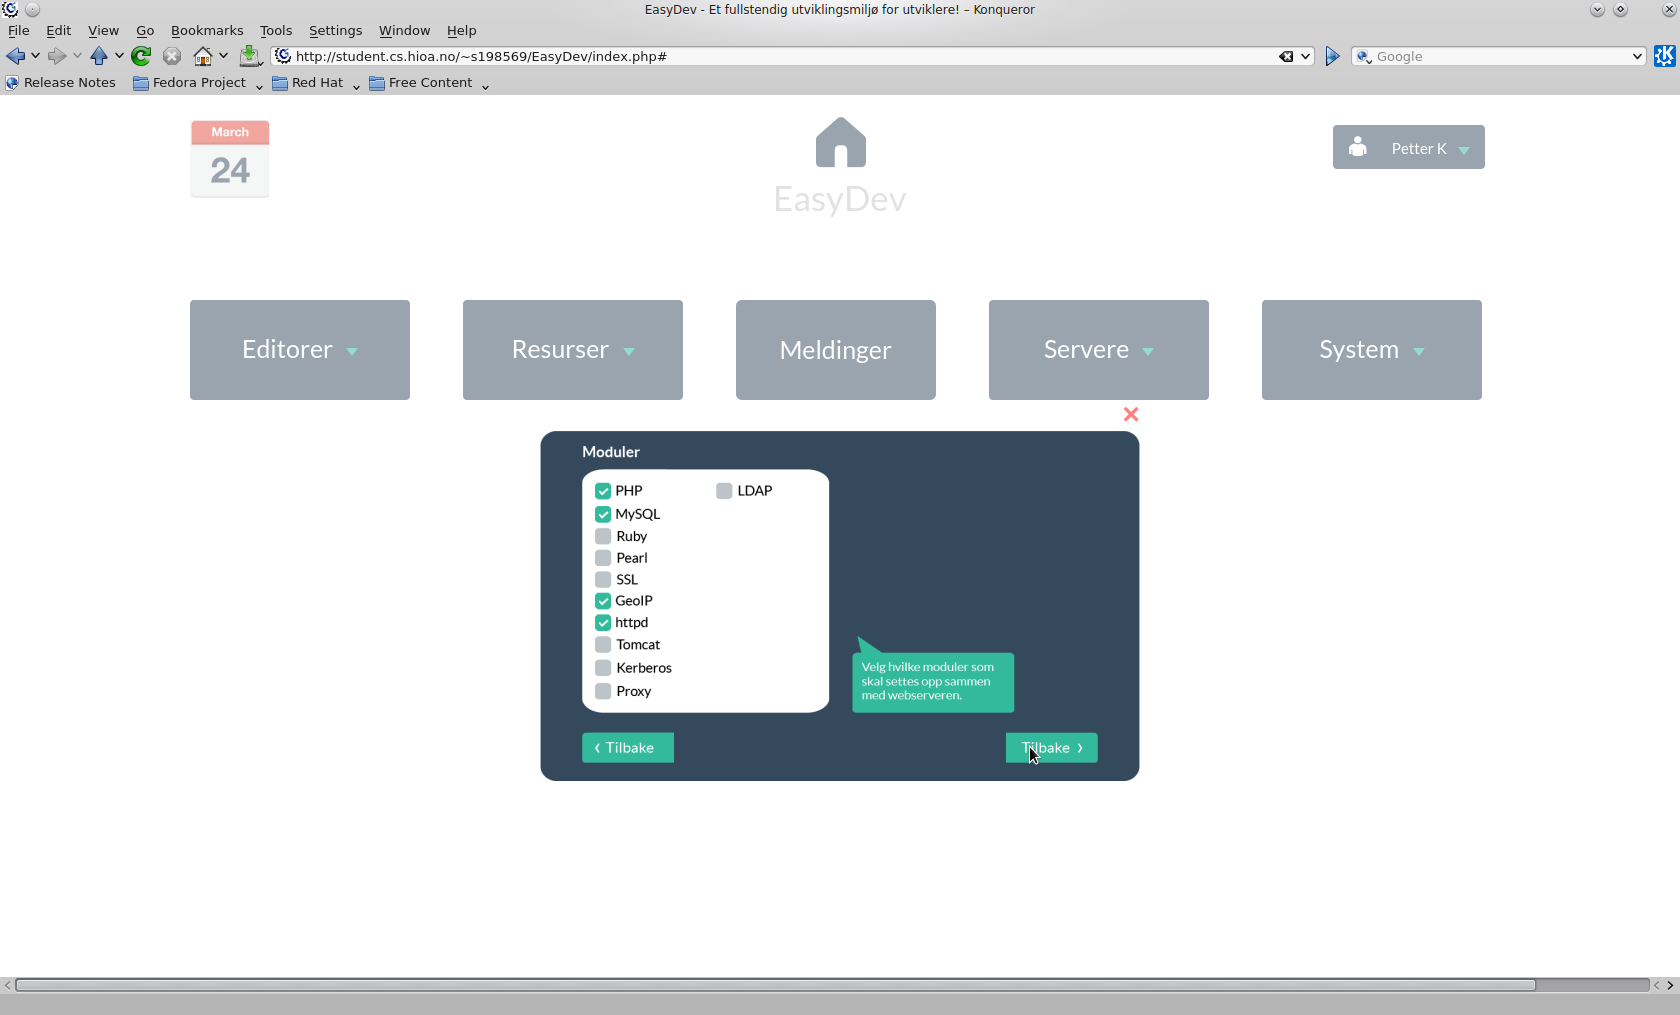
\includegraphics[width=\textwidth,height=\textheight,keepaspectratio]{./img/prosessdokumentasjon/hifi/a4.png}
\caption{(Hi-fi) Webserver: }
\label{fig:apachehi4}
\end{figure}

\begin{figure}[ht]
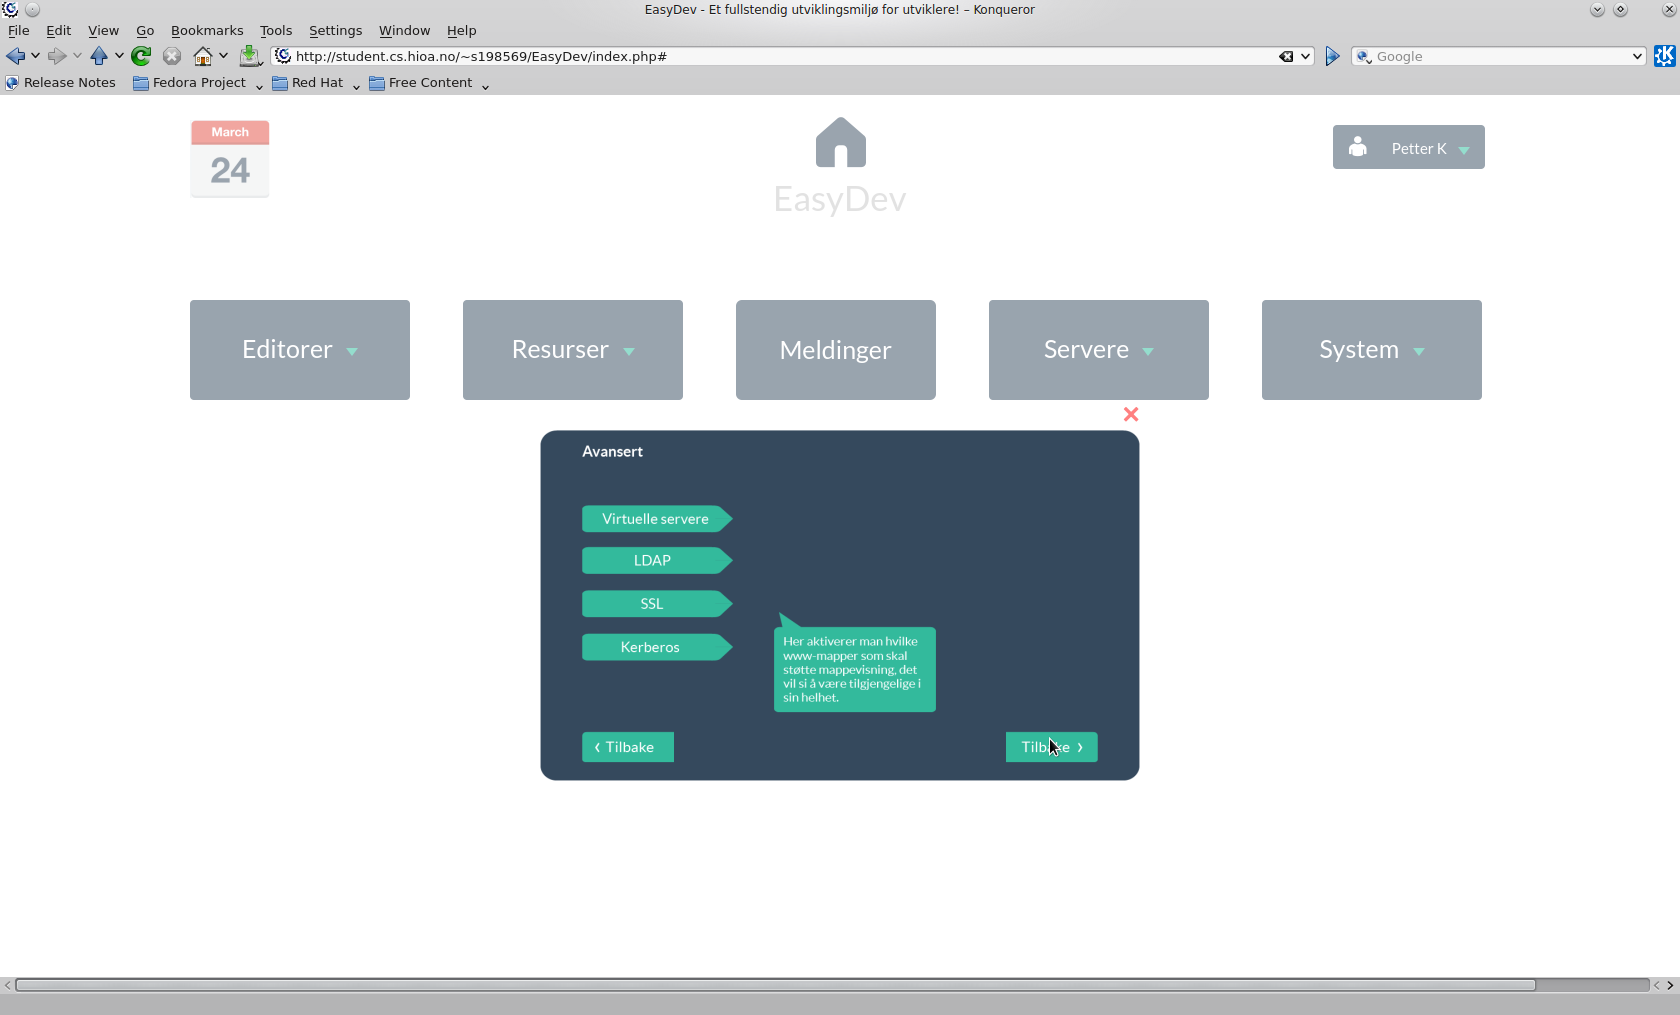
\includegraphics[width=\textwidth,height=\textheight,keepaspectratio]{./img/prosessdokumentasjon/hifi/a5.png}
\caption{(Hi-fi) Webserver:}
\label{fig:apachehi5}
\end{figure}

%KONFIGURASJON AV BRUKERE
\begin{figure}[ht]
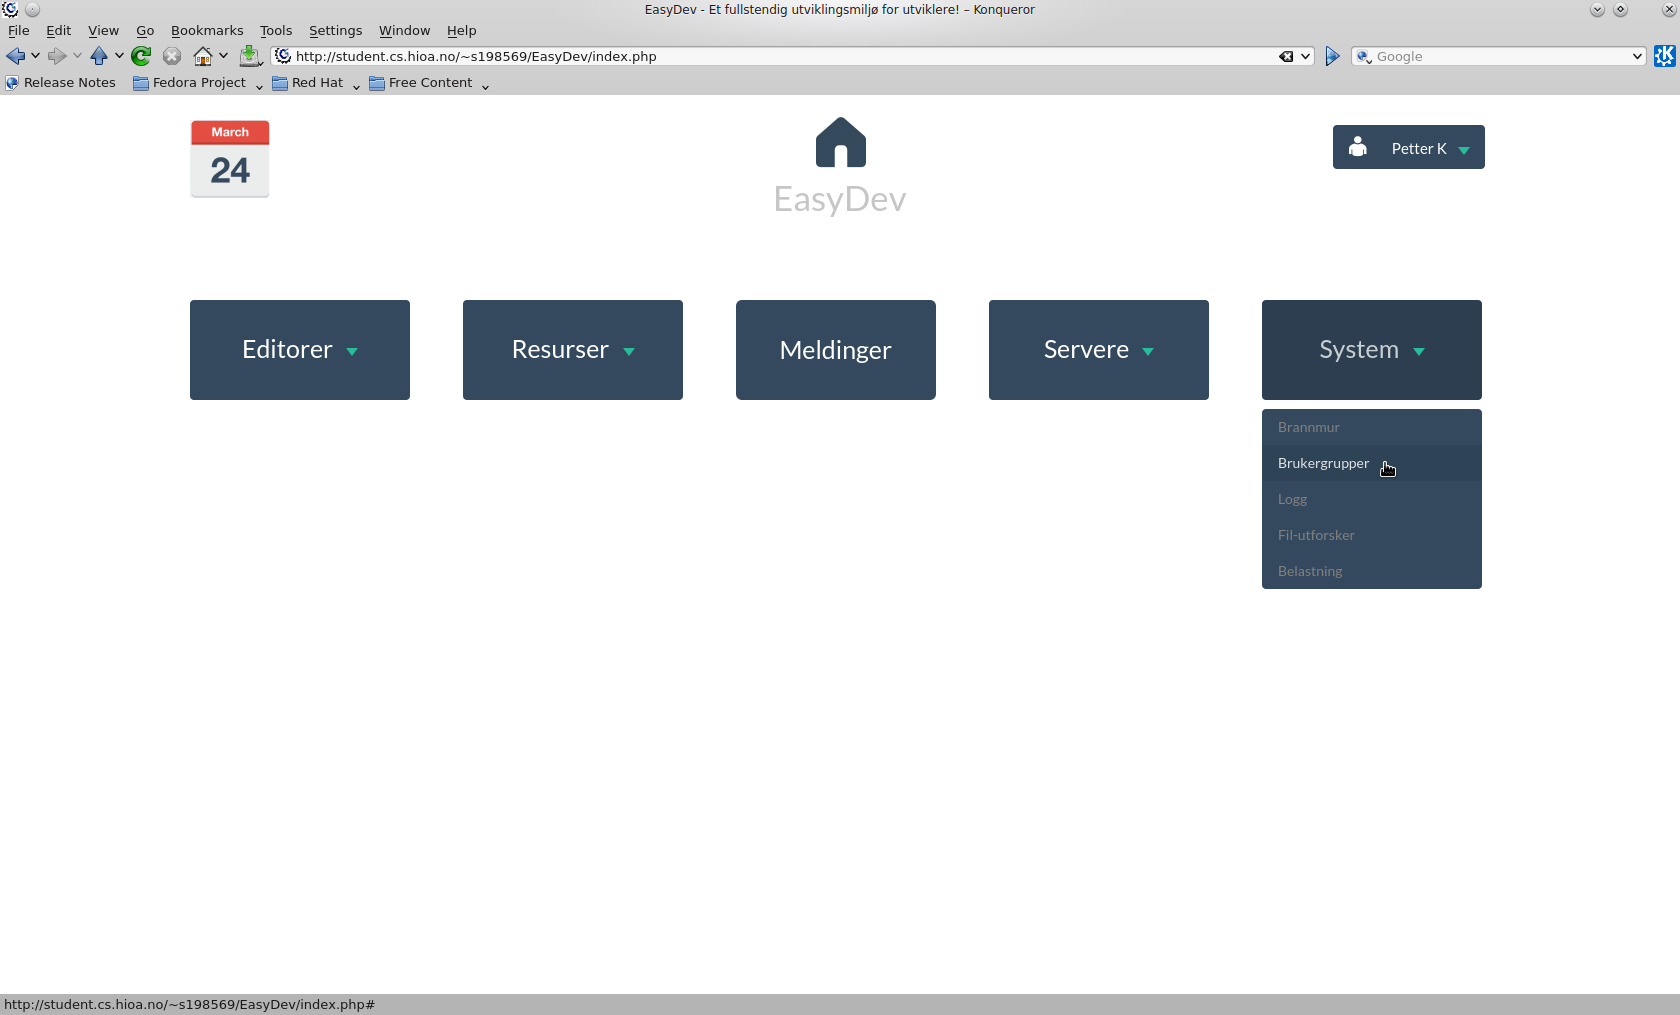
\includegraphics[width=\textwidth,height=\textheight,keepaspectratio]{./img/prosessdokumentasjon/hifi/b1.png}
\caption{Brukere: }
\label{fig:brukerehi1}
\end{figure}

\begin{figure}[ht]
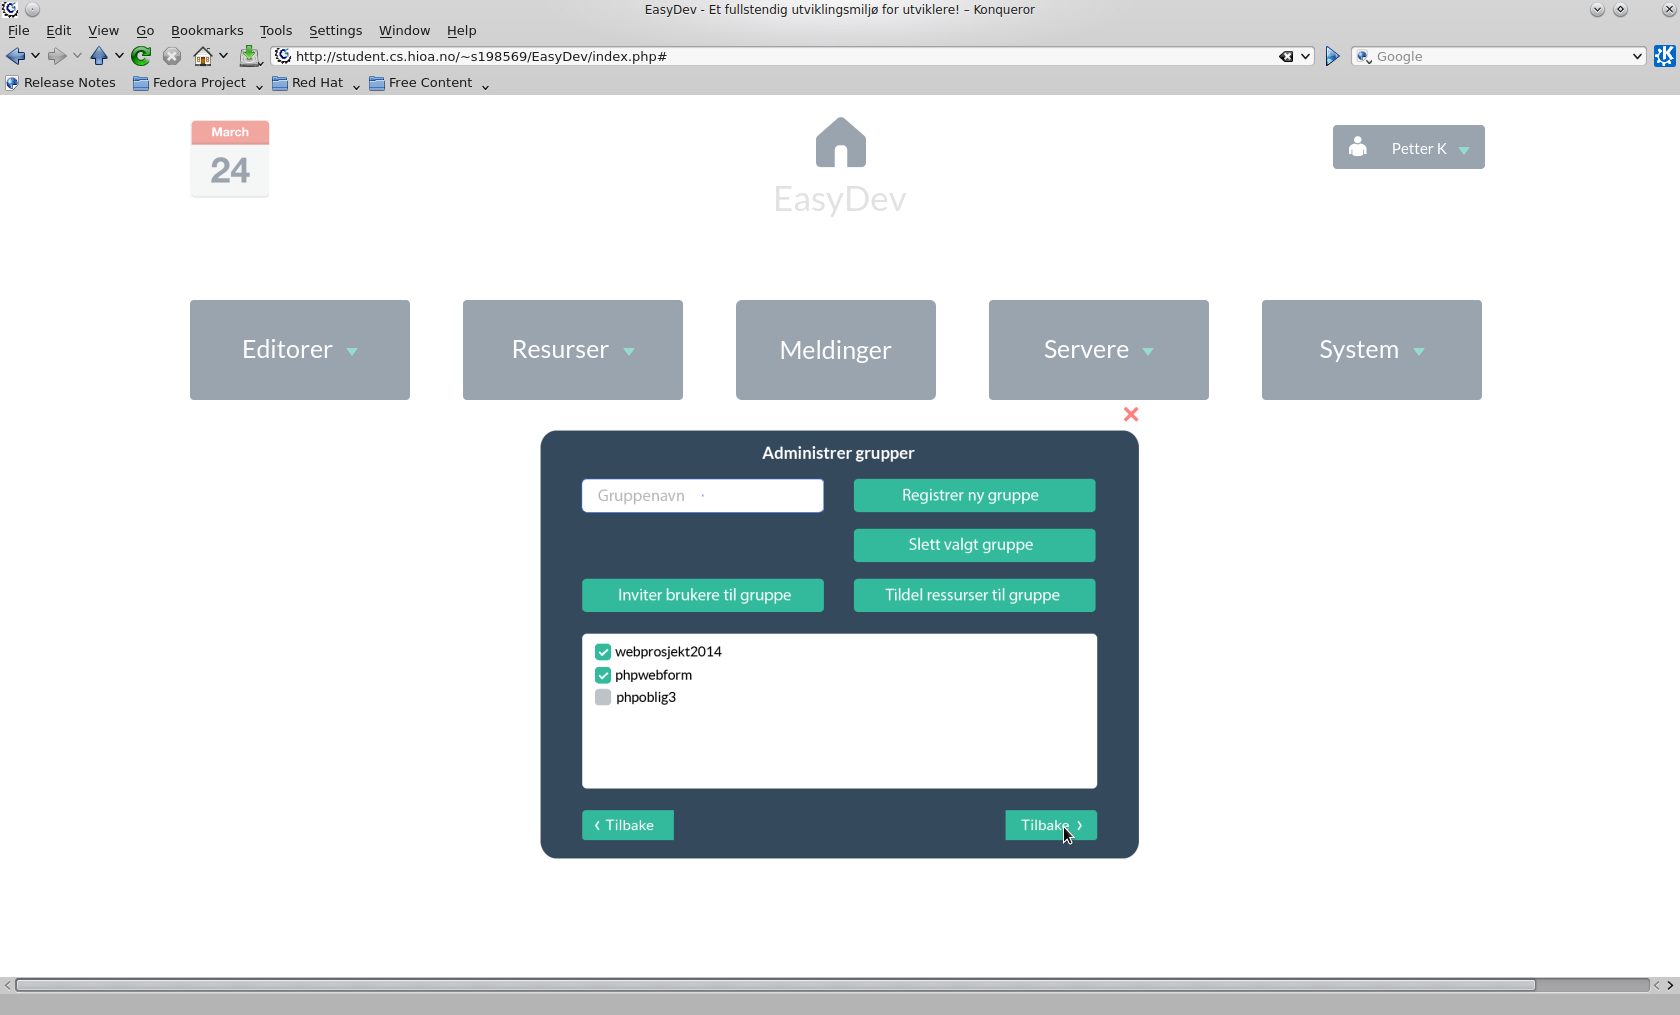
\includegraphics[width=\textwidth,height=\textheight,keepaspectratio]{./img/prosessdokumentasjon/hifi/b2.png}
\caption{Brukere: }
\label{fig:brukerehi2}
\end{figure}

\begin{figure}[ht]
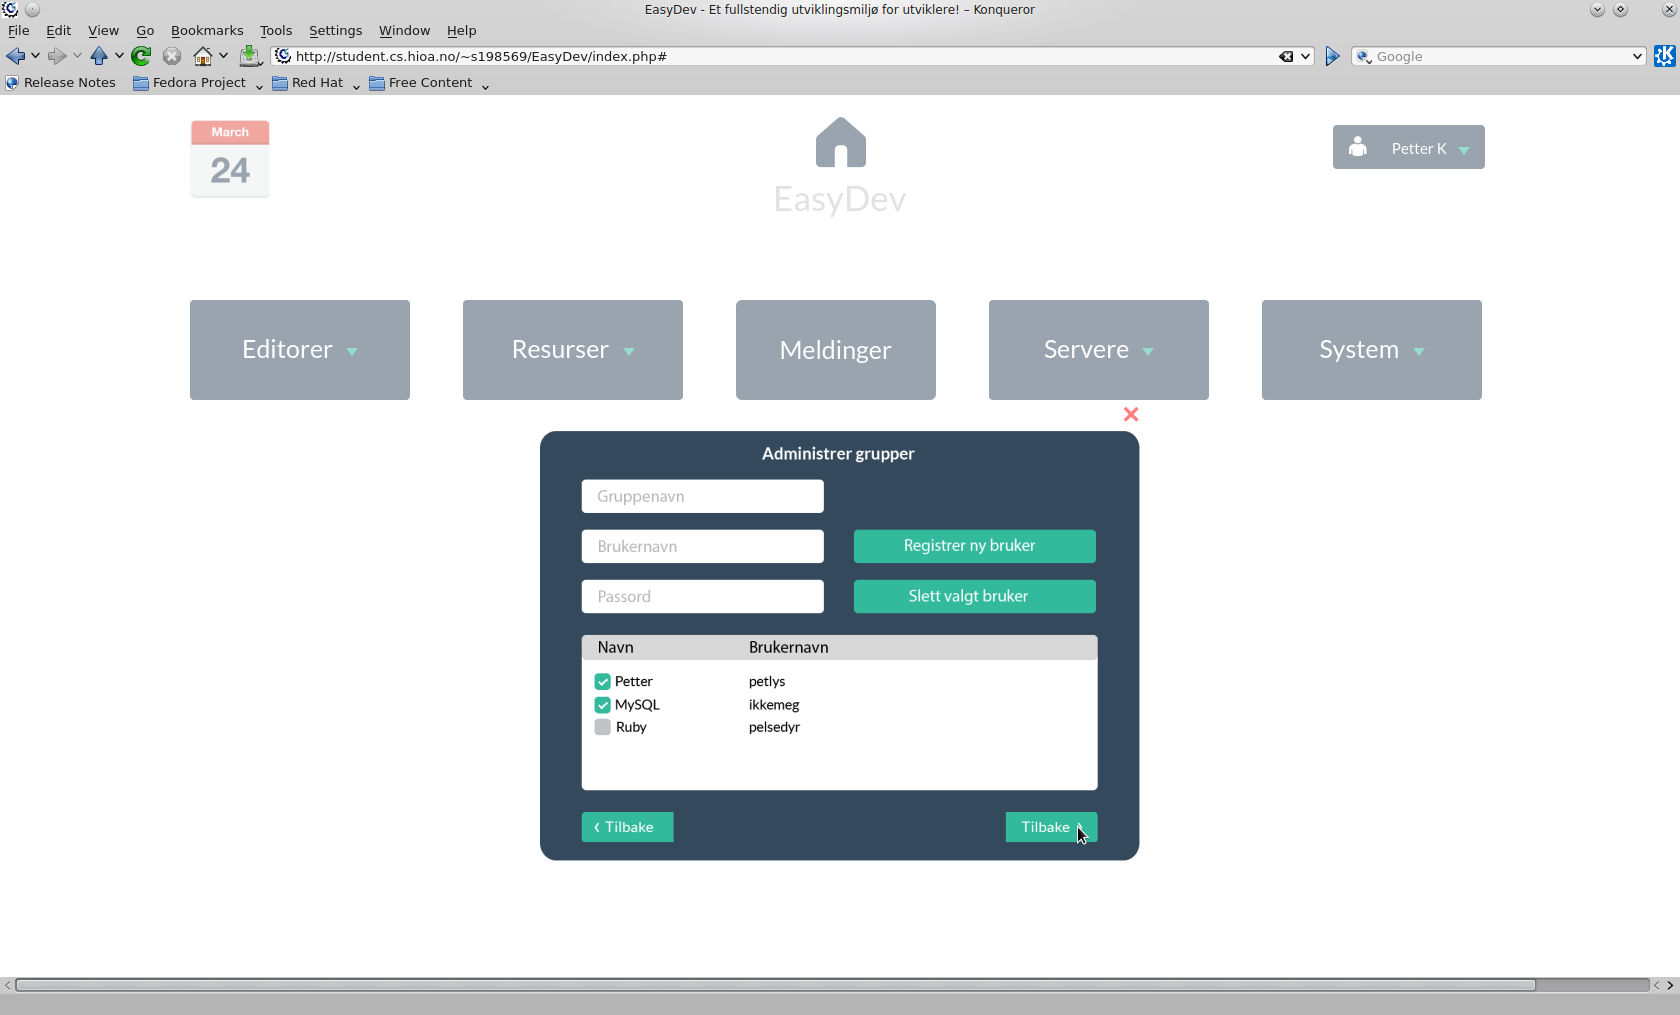
\includegraphics[width=\textwidth,height=\textheight,keepaspectratio]{./img/prosessdokumentasjon/hifi/b3.png}
\caption{Brukere: }
\label{fig:brukerehi3}
\end{figure}

\begin{figure}[ht]
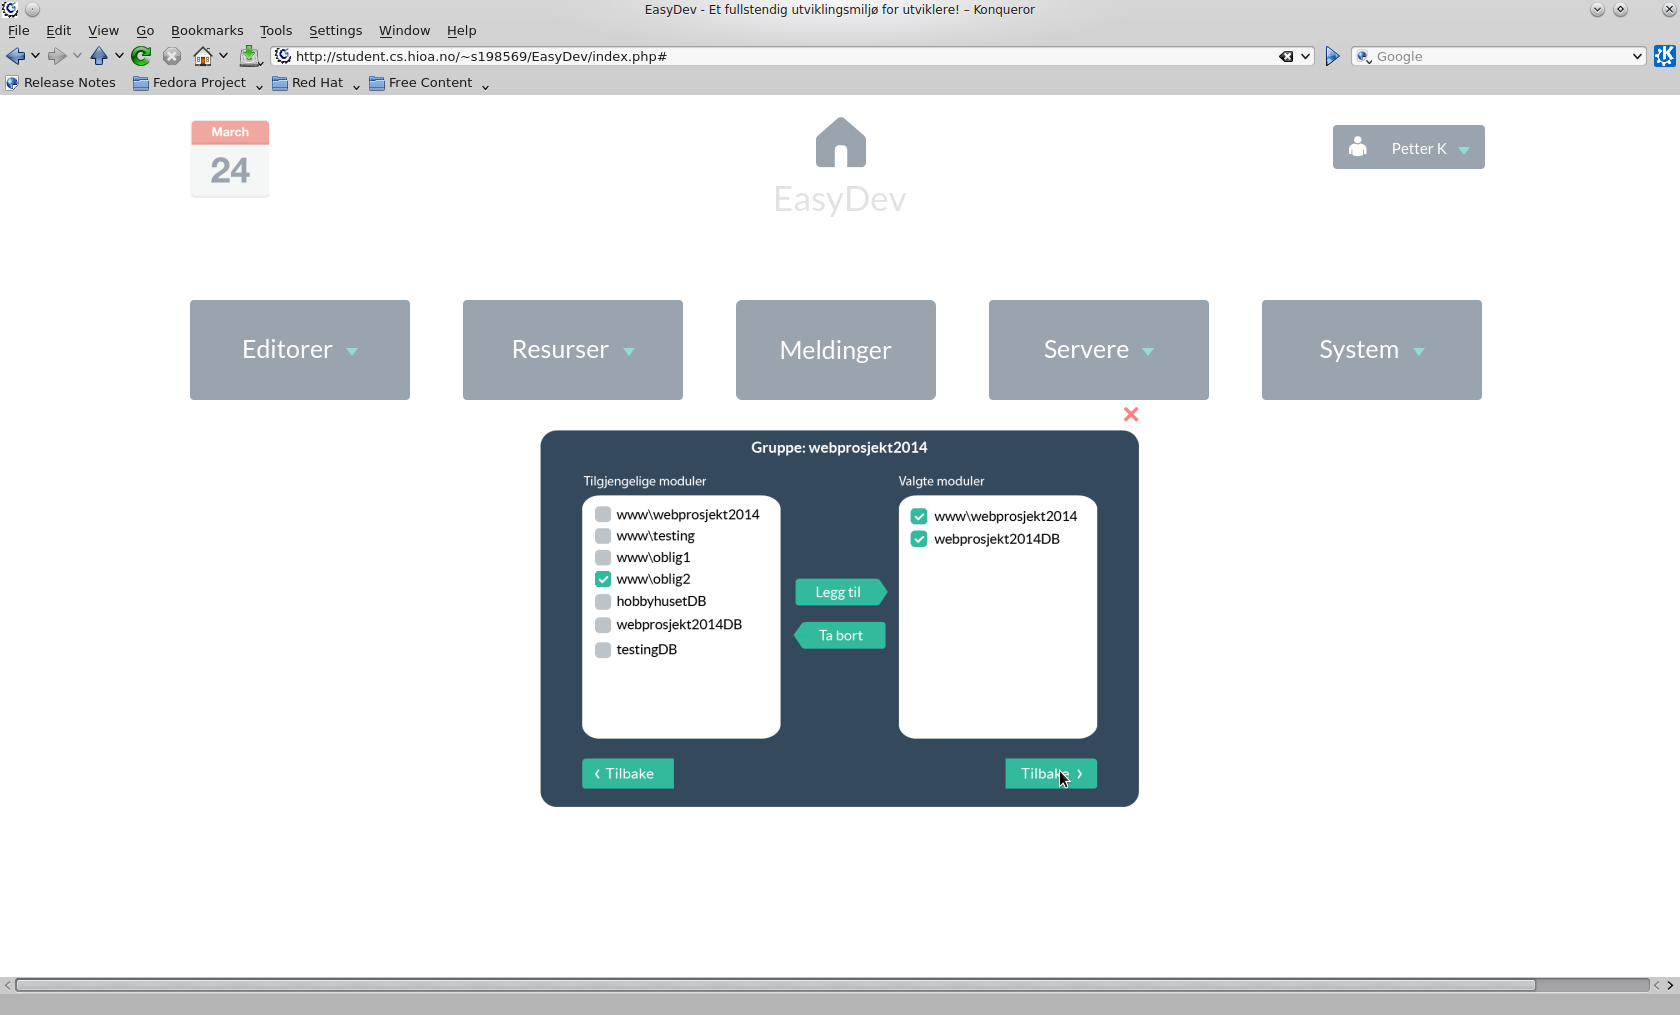
\includegraphics[width=\textwidth,height=\textheight,keepaspectratio]{./img/prosessdokumentasjon/hifi/b4.png}
\caption{Brukere: }
\label{fig:brukerehi4}
\end{figure}


% IKKE SLETT VIL HA DENNE SOM EKSEMPEL
%\begin{figure}[ht]
% 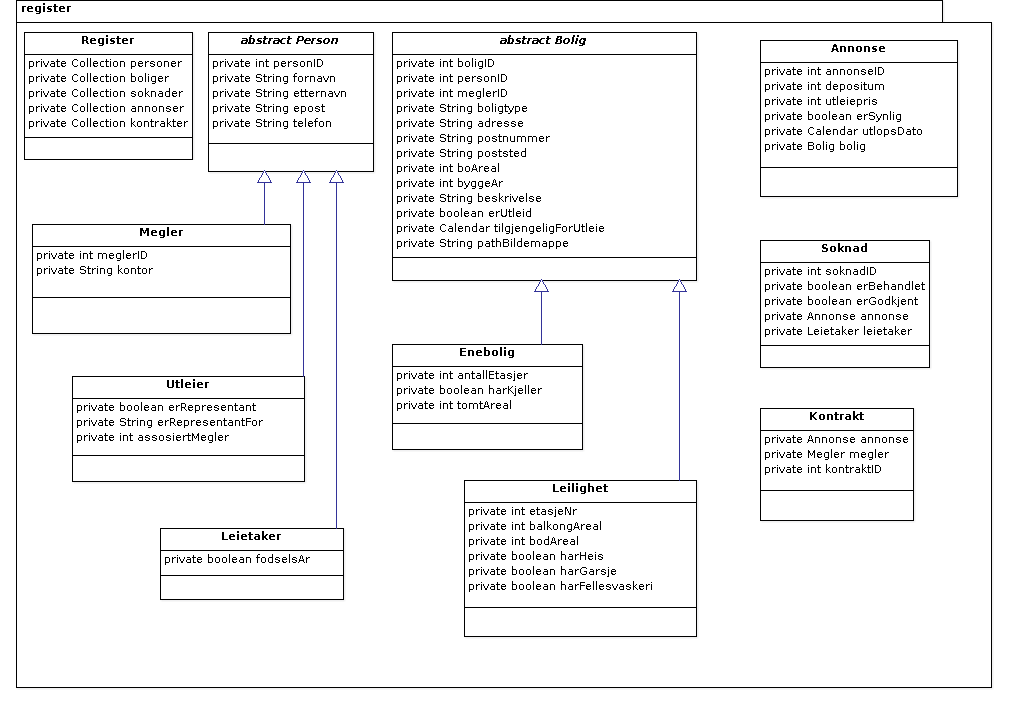
\includegraphics[angle=90 ,width=\textwidth,height=\textheight,keepaspectratio]{./img/appendix/diagram/klassestruktur_uml.png}
% \caption{Innledende UML diagram. brukt for generering av grunnleggende klasser.}
% %Her kommer en kabel for kryssreferering i teksten til figuren
% \label{fig:uml_diag}
%\end{figure}
\end{document}